%% FEUP THESIS STYLE for LaTeX2e
%% how to use feupteses (English version)
%%
%% FEUP, JCL & JCF, 31 July 2012
%%
%% PLEASE send improvements to jlopes at fe.up.pt and to jcf at fe.up.pt
%%

%%========================================
%% Commands: pdflatex tese
%%           bibtex tese
%%           makeindex tese (only if creating an index) 
%%           pdflatex tese
%% Alternative:
%%          latexmk -pdf tese.tex
%%========================================

\documentclass[11pt,a4paper,twoside,openright]{report}

%% For iso-8859-1 (latin1), comment next line and uncomment the second line
\usepackage[utf8]{inputenc}
%\usepackage[latin1]{inputenc}

%% English version

%% MIEIC options
%\usepackage[mieic]{feupteses}
\usepackage[mieic,juri]{feupteses}
%\usepackage[mieic,final]{feupteses}
%\usepackage[mieic,final,onpaper]{feupteses}

%% Additional options for feupteses.sty: 
%% - onpaper: links are not shown (for paper versions)
%% - backrefs: include back references from bibliography to citation place

%% Uncomment the next lines if side by side graphics used
\usepackage[lofdepth,lotdepth]{subfig}
\usepackage{graphicx}
\usepackage{float}
\usepackage{url}
\urlstyle{same} 

%% Include color package
\usepackage{color}
%\usepackage{float}
%\usepackage{subfig}
\usepackage[justification=centering]{caption}
\definecolor{cloudwhite}{cmyk}{0,0,0,0.025}

%% Include source-code listings package
\usepackage{listings}
\lstset{ %
 language=C,                        % choose the language of the code
 basicstyle=\footnotesize\ttfamily,
 keywordstyle=\bfseries,
 numbers=left,                      % where to put the line-numbers
 numberstyle=\scriptsize\texttt,    % the size of the fonts that are used for the line-numbers
 stepnumber=1,                      % the step between two line-numbers. If it's 1 each line will be numbered
 numbersep=8pt,                     % how far the line-numbers are from the code
 frame=tb,
 float=htb,
 aboveskip=8mm,
 belowskip=4mm,
 backgroundcolor=\color{cloudwhite},
 showspaces=false,                  % show spaces adding particular underscores
 showstringspaces=false,            % underline spaces within strings
 showtabs=false,                    % show tabs within strings adding particular underscores
 tabsize=2,	                    % sets default tabsize to 2 spaces
 captionpos=b,                      % sets the caption-position to bottom
 breaklines=true,                   % sets automatic line breaking
 breakatwhitespace=false,           % sets if automatic breaks should only happen at whitespace
 escapeinside={\%*}{*)},            % if you want to add a comment within your code
 morekeywords={*,var,template,new}  % if you want to add more keywords to the set
}

%% Uncomment to create an index (at the end of the document)
%\makeindex

%% Path to the figures directory
%% TIP: use folder ``figures'' to keep all your figures
\graphicspath{{figures/}}

%%----------------------------------------
%% TIP: if you want to define more macros, use an external file to keep them
%some macro definitions

% format
\newcommand{\class}[1]{{\normalfont\slshape #1\/}}

% entities
\newcommand{\Feup}{Faculdade de Engenharia da Universidade do Porto}

\newcommand{\svg}{\class{SVG}}
\newcommand{\scada}{\class{SCADA}}
\newcommand{\scadadms}{\class{SCADA/DMS}}

%%----------------------------------------

%%========================================
%% Start of document
%%========================================
\begin{document}

%%----------------------------------------
%% Information about the work
%%----------------------------------------
\title{Journata - Designing the interaction of a mobile application for exchanging public transport information among travellers}
\author{Marco André Moreira Amador}

%% Uncomment next line for date of submission
\thesisdate{June 23, 2014}

%%Uncomment next line for copyright text if used
%\copyrightnotice{Name of the Author, 2008}

\supervisor{Advisor}{Teresa Galvão Dias (Prof.)}
\supervisor{Co-Advisor}{António Nunes (MSc.)}

%% Uncomment next line if necessary
%\supervisor{Second Supervisor}{Name of the Supervisor}

%% Uncomment committee stuff in the final version if used
%\committeetext{Approved in oral examination by the committee:}
%\committeemember{Chair}{Doctor Name of the President}
%\committeemember{External Examiner}{Doctor Name of the Examiner}
%\committeemember{Supervisor}{Doctor Name of the Supervisor}
%\signature

%% Specify cover logo (in folder ``figures'')
\logo{uporto-feup.pdf}

%% Uncomment next line for additional text  below the author's name (front page)
%\additionalfronttext{Preparação da Dissertação}

%%----------------------------------------
%% Preliminary materials
%%----------------------------------------

% remove unnecssary \include{} commands
\begin{Prolog}
  \chapter*{Abstract}

The advent of smartphones and the massification of Internet connections allowed easy access and sharing of real-time information between people. That contributed to the success of several social networks and location-based services developed for mobile devices. The change of paradigm to accessing and sharing information may be explored in order to solve mobility problems, through improvements on public transport services and their use experience, promoting the use of public transport in urban areas.

In these terms, a proposal was made in order to create a mobile application, with social network features, allowing real time sharing of public transport information between travellers, with such information being related to several aspects of the service. Sharing that sort of information can be useful to a better informed decision making by the users about their own journeys, and form a way that public transport operators can use in order to gather information about their service quality and, therefore, to improve it. Simultaneously, a good structure and organization of the shared information maximizes its utility to the users of the platform. The previous work resulted in a functional prototype with several limitations concerning the usability and user interaction with the application, conditioning the application's engagement and mass adherence by potential users.

This dissertation aims to develop a functional prototype to said application, applying user-centred design processed in order to produce a new iteration that overcomes the referred limitations, improving user experience and focusing in the interaction between the final user and the application. Initially, it was performed the elicitation of the limitations of the previous iteration of the application, along with some research in order to understand the usability requirements among potential users. After the prototype development (through an iterative process with evolution and validation of the designed interface and interaction), usability tests were performed among experts in the field of mobile applications development to public transport systems, which allowed to gather feedback about the work carried out and the potential range of an application such as this.

This work can be seen as an evolution of the base concept behind this application, based upon user engagement in the development process phases, serving as a starting point to the integration of the addressed concepts in larger scale projects related to mobility.

\chapter*{Resumo}

O advento dos smartphones e a massificação das conexões à Internet possibilitou às pessoas o acesso e partilha de informação em tempo real com facilidade. Tal contribuiu para o sucesso de várias redes sociais e outros serviços baseados na localização do utilizador de dispositivos móveis. A alteração desse paradigma de acesso e partilha de informação poderá ser explorada no intuito de resolver problemas associados à mobilidade, através da melhoria dos serviços de transporte público e da sua experiência de utilização, promovendo a utilização desse tipo de transporte.

Nesse sentido, foi proposta anteriormente a criação de uma aplicação móvel com características de rede social com vista à troca de informações de transportes públicos entre os seus passageiros, em tempo real, sendo essas informações referentes a vários aspectos do serviço. A partilha desse tipo de informações poderá ser útil para uma tomada de decisão mais informada acerca das suas viagens, por parte dos utilizadores, e constituir uma forma através da qual os operadores de transporte público poderão recolher informação sobre o seu serviço com vista a melhorar a qualidade do mesmo. Simultaneamente, a estruturação e organização da informação partilhada maximiza a utilidade da mesma para os utilizadores da plataforma. Esse trabalho anterior resultou num protótipo funcional com severas limitações na óptica de usabilidade e interacção com o utilizador, o que condiciona uma adesão da mesma em larga escala por parte de potenciais utilizadores.

Esta dissertação tem como objectivo o desenvolvimento de um protótipo funcional para a dita aplicação, aplicando os processos de design centrado no utilizador de modo a produzir uma nova iteração dessa aplicação que ultrapasse essas limitações, melhorando a experiência de utilização e dando foco à interacção entre a aplicação e o utilizador final. Inicialmente, foi feito o levantamento das limitações da iteração anterior da aplicação móvel, tendo sido igualmente feita alguma pesquisa no sentido de perceber quais os requisitos de usabilidade de potenciais utilizadores. Após o desenvolvimento do referido protótipo (através de um processo iterativo com evolução e validação da interface e interacção concebidas), foram realizados testes de usabilidade, junto de experts na área do desenvolvimento de aplicações móveis para transportes públicos, o que permitiu recolher feedback acerca do trabalho realizado e do possível alcance de uma aplicação deste tipo. Este trabalho pode ser visto como uma evolução do conceito base desta aplicação, tendo por base o envolvimento dos utilizadores nas fases do processo de desenvolvimento, servindo de ponto de partida para a integração dos conceitos aqui abordados em projectos de maior escala ligados à mobilidade.
 % the abstract
  \chapter*{Acknowledgements}

I would not be able to accomplish this work without the priceless contribute from a lot of people to whom I am grateful.

First of all, I would like to thank my family, specially my parents and my grandfather, for all the constant support and the help to find motivation when I needed the most, and, most importantly, for the opportunity that was given to me in order to choose this field of study in this faculty. Without them and their sacrifice, it would not be possible, and I'll never forget that. I sure hope to have seized that opportunity in the right way.

To my friends and colleagues, the most amazing group of people I have met, I cannot thank you enough for being there for me, even in the worst moments. It was an immense privilege to be at your side during this course. Thanks for giving me strength to always carry on during the course, and for all the countless help. Without you, I probably wouldn't be writing this now. And Eduardo, you'll never be forgotten!

To my supervisor, Prof. Teresa Galvão, for all the support and precious advice, for all the valuable suggestions and the availability in the difficult times.

To Eng. António Nunes, my co-supervisor, for always being there to help and contribute with his valuable input, giving great advice and ideas for this work's development. His curiosity inspired me to explore new types of possible solutions to overcome the challenged presented in this work. I surely hope to have meet his expectations, because this project is born from his idea and because I recognise the great potential of this project.

To all the people at CAS, for making me comfortable and providing a great place to work.

To OPT, thanks for all the expertise and valuable feedback given in the final testing phase, and all the demonstrated interest in the project.

To the users of Stack Overflow, who 'saved my life' several times during the implementation phase of this work. Without that platform as a valuable help tool, the amount of work accomplished would surely be less.

Finally, I would like to thank all the people that took some of their own time to participate in the focus group and the usability testing. Without them, this work would not be possible for sure.



\vspace{10mm}
\flushleft{Marco Amador}
  % the acknowledgments
  \cleardoublepage
\thispagestyle{plain}

\vspace*{8cm}

\begin{flushright}
   \textsl{``The brick walls are there for a reason.
   The brick walls are not there to keep us out.
   The brick walls are there to give us a chance to show how badly we want something.
   The brick walls are there to stop the people who don’t want it badly enough.''} \\
\vspace*{1.5cm}
           Randy Pausch
\end{flushright}
       % initial quotation if desired
  \cleardoublepage
  \pdfbookmark[0]{Table of Contents}{contents}
  \tableofcontents
  \cleardoublepage
  \pdfbookmark[0]{List of Figures}{figures}
  \listoffigures
  \cleardoublepage
  \pdfbookmark[0]{List of Tables}{tables}
  \listoftables
  \chapter*{Abbreviations}
\chaptermark{ABBREVIATIONS}

\begin{flushleft}
\begin{tabular}{l p{0.8\linewidth}}
API      & Application Programming Interface\\
IBM-CAS  & IBM Center for Advanced Studies \\
C2DM     & Google Cloud to Device Messaging Framework \\
GCM      & Google Cloud Messaging Framework \\
GPS      & Global Positioning System \\
GSM      & Global System for Mobile Communications \\
ISO      & International Organization for Standardization \\
NFC      & Near Field Communication \\
OS       & Operative System \\
QRCode   & Quick Response Code \\
STCP     & Sociedade de Transportes Colectivos do Porto \\
TFL      & Transport for London \\
UI       & User Interface \\
UX       & User Experience \\
XML      & Extensible Markup Language \\




\end{tabular}
\end{flushleft}

  % the list of abbreviations used
\end{Prolog}

%%----------------------------------------
%% Body
%%----------------------------------------
\StartBody

%% TIP: use a separate file for each chapter
\chapter{Introduction} \label{chap:intro}

\section*{}

This initial chapter aims to give a general overview about this thesis and the themes it addresses. It will start by explaining the context in which it is inserted, as well as the motivation beneath the proposal.

The main objectives of this thesis, as well as the methods that will be employed in order to achieve them, will also be described.



\section{Context} \label{sec:context}

In the last few years, we have seen the speed of evolution and innovation regarding technology to reach levels we never thought before, applied to several fields. One of these fields, and probably the one where we, as human beings, felt more that evolution was communication. 
Some of the big changes we perceived was for instance, the massification of the e-mail usage to communicate, the rise of instant messaging applications, the boost of the number of mobile phones and Internet connections worldwide ~\cite{kn:Int13}.

Some studies \cite{kn:DMW03} related to the "Six Degrees of Separation theory", which defends that every person in the Earth is only separated, through an introduction process, by six steps to any other person, have shown that the value for average number of steps between any given people has been decreasing in the last few years. Microsoft itself performed a study with data from Messenger application, that revealed, only using that application, that the mean path between Messenger users is 6.6 \cite{kn:LH07}.

The advent of social networks, platforms that allow information sharing and interaction between people in several ways, had (and still has) a great contribute in approximating people and, along with the growth of Internet connections worldwide and the easiness of internet access, allows people to be constantly connected and communicating.

Mobile devices, in the last few years, have evolved as well, along with technology, developing capabilities of internet access and allowing that connection and communication to be done even when people are not at home or at work.

As this evolution happens, we witness as well an increasing migration from people to larger cities, promoting an increment on the worldwide population living in urban areas. Recent data on this migration show that this migration is happening in both well developed and less developed regions around the globe \cite{kn:NAT11}.

This is contributing to generate some chaos in our cities, making the task of quickly reaching our destinations increasingly harder,due to the increasing number of vehicles and people.

In this context, public transportation has a vital role on promoting urban mobility and helping us to avoid those problems. Encouraging its use reduces the number of cars, thus reducing traffic levels and the likelihood of traffic jams, increasing the efficiency of mobility inside the cities and the efficiency of public transport system itself \cite{kn:CSV11}.

As an attempt to promote public transport usage, some companies publicize their services and try to reach their costumers through social networks, particularly the most widely used, such as \emph{Facebook}\footnote{\url{http://www.facebook.com}} or \emph{Twitter}\footnote{\url{http://www.twitter.com}}, taking advantage of their popularity.

The concept that supports this thesis is based upon this phenomenon, and tries to explore social network's abilities to act as information vehicle between people, and the willingness of people to share information in the first place. However, the kind of information we intend to see shared between people with this project is information concerning public transport, in such way that both users and operators can benefit from that information. 

This concept has been proposed in the article \emph{Using social networks for exchanging valuable real time public transport information between travellers} \cite{kn:NGeCP11}, and its implementation is in course at the \emph{IBM Center for Advanced Studies} at FEUP. That implementation has been the subject of previous master thesis works from MIEIC, and resulted on a prototype for an Android mobile application \cite{kn:eSG12}. 

This thesis aims to provide a redesigned and intuitive interface to the project, in order to make the new iteration a more efficient way for travellers to help each other and contribute to a better public transport service, ultimately leading to an increasing use of public transport (and possibly more efficient public transport and cities). 

\section{Motivation} \label{sec:motivation}

Time is a very important resource nowadays, specially for those who live in a city. We waste some of that time on our daily travels, such as performing home-to-work journeys and the reverse. Often, journeys that should last 10 minuted end up lasting much more than that, due to delays, traffic jams and so on. 

Those factors generate some unpredictability on public transport behaviour that, allied with the lack of information about the routes, delays and unexpected problems, frequently leads people to try to avoid them when possible, in order to keep up to their schedule \cite{kn:BC07}.

Providing travellers with real-time status information about public transport is something that can lead people to use them. This way, we can help people making informed travel decisions, while possibly reducing the number of private vehicles circulating in our cities, thus reducing traffic and saving time. It can also lead to improvements in the usage experience of public transportation by the travellers, resulting in more bearable waits and journeys.

Social networks have been used in the recent times by some public transport companies in order to get closer to their customers and to provide them some real-time information about their services. Using social networks, those companies are establishing a two-way communication street with their customers, generating feedback that can be used to improve the quality of the offered services.

However, recent studies have shown that, despite the notorious advantages that arise from this kind of approach, the information provided is not fully exploited sometimes, leading users to perceive it as useless and to underestimate it \cite{kn:NGeCP11}.

The existence of a social network designed to provide structured information in real-time to the right people (people that would perceive that information as highly useful), through a mobile application, could help improving the public transport' perceived experience. Moreover, if the information shared inside this social network had origin in the users themselves, the transport operators wouldn't have charges related to the maintenance of those services, while receiving a constant source of feedback they can use to improve the quality and efficiency of their services.

This social network could also contribute to other kinds of benefits (apart from the economical ones to the transport operators\cite{kn:NGeC14}). For instance, it could lead to decreasing levels of stress suffered by passengers of public transport, by increasing their well-being, and also, as an ultimate consequence, to the reduction of the ecological footprint generated by the widespread use of private vehicles on home-to-work travels.

However, providing structured information to the right people in real-time is not enough. Being this social network fed by information generated by and shared between its users, it must have as many users as possible, in order to generate a large volume of information, so that users can receive information useful for them.

That said, the user interface (UI) of the social network, in this case, a mobile application, must be intuitive and attractive to the passengers, captivating them to use it daily and to contribute to the information flow inside the social network. 

\section{Goals} \label{sec:goals}

One of the most innovative aspects of the concept referred in the last section is the creation of dynamic community networks, in time and space. For instance, in a social network such as \emph{Facebook}, we have a list of friends and acquaintances that does not change a lot over time (thus, forming static networks). In the proposed concept \cite{kn:NGeCP11}, it is discussed the creation of dynamic networks, representative of travellers on a specific line, vehicle, or inside vehicles from different lines that share part of its trip between them. That way, a traveller would only receive information from other travellers in the same networks, maximizing the utility of the received information.
The main goal of this thesis is to develop a user interface for the mentioned system, while achieving the following objectives:

\begin{itemize}
\item Create and analyse appropriate metaphors for the interaction with dynamic social networks.
\item Design and test innovative visual affordances for the concept of dynamic social networks.
\item Apply state-of-the-art concepts related with Human-Computer Interaction in order to maximize the usability of the application by its final users, while addressing usability problems identified on the previous existing prototype.
\item Develop a functional prototype for an Android mobile application based on the obtained from the goals already mentioned.
\item Test the system and evaluate the results obtained.
\end{itemize}

\section{Structure of the Report} \label{sec:struct}

Besides the Introduction chapter, this document contains six additional chapters, with the following structure:
%\todoline{Complete the document structure.}
Chapter \ref{chap:chap2}, \emph{State-of-the-Art}, presents the definition, explanation and related works in the fields of the concepts in which the project is based upon. It will also present examples of several mobile applications with social network features and/or related to public transport information.

Chapter \ref{chap:chap3}, \emph{Problem Description and Approach}, explains more in detail what is meant to achieve with this work and the problem that is discussed in it, as well as the chosen approach to reach the proposed goals.

Chapter \ref{chap:chap4}, \emph{Requirements Elicitation}, describes the work performed in the initial phase of the process, having the previous state of the project as a starting point to some new design proposals, and the realization of a focus group to perceive user needs and usability requirements.

Chapter \ref{chap:chap5}, \emph{Application}, presents the architecture of the application, and describes the evolution of each main design concept of it, from the first sketches to the implementation phase.

All the performed tests and subsequent results are presented in Chapter \ref{chap:chap6}, \emph{Tests and Results}.

Finally, Chapter \ref{chap:chap7} presents the conclusions taken from this thesis, as well as suggestions about future work to be done in the project and ways it can evolve in order to maximize its reach, and  be integrated with bigger scale solutions.
 
\chapter{State-of-the-Art} \label{chap:chap2}

\section*{}

Social networks are changing the paradigm of communication between people. We have seen an increasing growth of the number of people using them in the past few years, and the same applies for the amount of time spent by people in these communities. This popularity brings a huge potential to these platforms, for instance, for promoting or marketing of products, sharing various kinds of information, and stimulating the collaboration among its users.
Using this strong sharing component, and with the help of some other features for communication between people, such as chat, instant messaging, video-conferencing and so on, these platforms develop some features of collaborative environments, making them attractive to implement the concept of Collective Intelligence \cite{kn:CSV11}. 

The fact that we can use a communication network everywhere these days had an impact on the social networks growth, popularity, and volume of information shared. To be online anywhere and at any moment, has become an habit for millions of human beings, and the smartphones' expansion had a great contribution to that. 
However, their increasing popularity does not exactly mean that people are easily driven or compelled to use new ones. Instead, they usually get bored faster and their acceptance of different networks and environments diminishes. 

So, in order to succeed, a new player, in this case, a new social network or platform, has to find new ways in order to keep people addicted to their services, and attract even more people.  We will start by clarifying some concepts that are in some way related with the project.

\section{Online Collaboration Tools}\label{sec:onlinecol}

Nowadays, we have a wide range of tools we can use to perform some kind of online collaboration, such as real-time collaborative text editors (Google Drive, for instance), wikis, Q\&A websites (\emph{StackOverflow and SuperUser} have an enormous success inside the IT community, allowing people to ask questions and to say problems they're facing and see them answered by someone with expertise on the field), and so on.

Most of these platforms, and their success, rely heavily on their number of users, on their features, and on the information flow generated and shared by them. In cases where the shared information is made public (Q\&A websites, for instance), the "community sense" perceived by the user, along with the value of the existing information, is fundamental to the acceptance of the platform.

That kind of collaboration lies deeply within the concept of Collective Intelligence, emerged from the debates held by Pierre Lévi \cite{kn:Le98}, where it is assumed that the intelligences of each individual are added and shared by the society.

\begin{quote}
"What is collective intelligence? It is a form of universally distributed intelligence, constantly enhanced, coordinated in real-time, and resulting in the effective mobilization of skills... My initial premise is based on the notion of a universally distributed intelligence. No one knows everything, everyone knows something, all knowledge resides in humanity." 
\end{quote}

This is something meant to be explored deeply in this thesis and the concept behind it, due to the functionality and usability the application aims to give to the passengers, in order to keep them generating useful information for other users.

The growth of online collaboration lead also to the growth of a new business model, called \emph{crowdsourcing}, where people submit problems to a community , instead of solving them on their own, hoping for the community to reply with better and/or more creative solutions.

That business model has also evolved into several sub-types, such as \emph{crowdfunding}, where someone prompts the community with a solution for a problem and asks the members of the community for funding, in order to develop and launch said solution, if the said members think the solution is viable, creative and/or necessary.

\section{Mobile Environment Overview}\label{sec:mobove}

As said before. we live in an era where smartphones allowed us to take advantages of the massification of wireless networks in order to be online, anywhere and at any given time.

They also allowed us to perform tasks we didn't imagine ourselves performing from a mobile phone twenty years ago, such as:

\begin{itemize}
\item Reading our e-mail account and send new e-mails.
\item Navigating on websites.
\item Share photos with friends via messages or social networks.
\item 'Check-in' at restaurants, clubs, museums, etc.
\item Use native applications to fetch several types of information: news, weather information, football scores, and even \emph{public transport information}, such as schedules.
\end{itemize}

The appearance of mobile operating systems with high number of default functionalities, such as Android \footnote{\url{http://www.android.com/meet-android/}} (maintained by Google) or iOS \footnote{\url{https://www.apple.com/ios/}} (from Apple Company), allied to the easy development of native applications for those OS's, lead to an exponential growth in the number of that type of devices worldwide and thus, their native applications.

Android is, by far, the mobile operating system with most devices sold and has a steep growing trend. It is known for being an open source Linux-based system, suitable for both smartphones and tablets and very flexible concerning to hardware configurations.

It has been well received by third-party phone manufacturers, and it has a large community of developers, as well as millions of native applications available for download. Users can find these application in their official store, \emph{Google Play Store}, the largest app store worldwide \cite{kn:Are13}, or through third-party websites.

Apple's iOS, however, is a closed-source system, for installation on Apple's devices only. 
It was originally developed for Apple's smartphones, iPhone, but it has since then been extended to other devices from the company, such as tablets (iPad) or portable music players (iPod Touch). Its application store is the most profitable worldwide.

Both Android and iOS have evolved since their first versions, not only adding functionality and features, but also providing developers with new methods to make their applications more usable, efficient and aesthetically attractive.

Mobile devices who have these operative systems are also equipped with a lot of embedded sensors, that provide help and data to some features of applications. Some of these sensors are:

\begin{itemize}
\item Motion Sensors (accelerometers, gyroscopes, gravity sensors);
\item Environmental Sensors (barometers, thermometers);
\item Position Sensors (orientation sensors, magnetometer);
\item Location Sensors (GPS sensors).
\end{itemize}

The last type of referred sensors, that allow the device and therefore its applications to detect and use information related to the users location, using GPS (\emph{Global Positioning System}), resulted in the creation of new types of services, that can be inserted in the Location-based Services category.

\section{Location-Based Services}\label{sec:lbs}

According to Kupper \cite{kn:Ku05}, there is no common definition or terminology for location-based services. Schiller and Voisar \cite{kn:SV04}, however, define location-based services as "services that integrate a mobile device's location or position with other information so as to provide added value to a user". 

GSM Association's definition is a little bit more abstract, and defines those services as "services that use the location of a client for adding value to the service".

In this context, the referred client is understood as any entity whose location is relevant, and not necessarily a mobile device or the user of the service.

This concept of location-based services, as it is known today, was first studied by Timo Rantalainen, in his master thesis in Electronical Engineering for Helsinki University of Technology, in 1994. In a posterior article \cite{kn:SR95}, he wrote about possible methods to determine users' location.

These services were created due to a set of particular questions that web developers faced with the growth of the Internet. For instance, how to adapt the contents of a website to a particular reader? Knowing their location (the country they were visiting the page from), it was made possible to display the website information in that country's language. In similar ways, results from a search engine could be customized to the user's country, as well as the advertisement shown \cite{kn:BWD11}.

The appearance of mobile computation brought new challenges to this area, and new strengths to these services - it is far more interesting to use the location of a mobile device than the location of a desktop computer, for instance.

Some of the biggest challenges were related to the way the location data was stored and handled (due to being from a mobile device and the data being dynamic, because the location is changing and the gathered data is continuous).

\section{Social Networks}\label{sec:sn}

In the definition provided by James Clyde Mitchell \cite{kn:Mit69}, a social network is a set of specific links between a group of people, with the additional property that the characteristics of these connections as a whole can be used to interpret the social behaviour of the involved individuals. 
Of course, this is the general definition of a social network, but nowadays we associate it to the phenomenon of online social networks, that according to the definition given by Nicole B. Ellison \cite{kn:BE08}, consist in Web services that allow an individual to:

\begin{itemize}
\item Create a public or semi-public profile within a bounded system;
\item Articulate a list of other users with whom they share a connection;
\item View and go through their list of connections and those made by others within the system.
\end{itemize}

However, most of these online platforms evolved beyond that definition, providing features to their users allowing them to upload content (for instance, photos, music or videos), send instant messages to other users and use small applications or play games \cite{kn:Joi08}.

Online social networks have grown in such a way that has provided them a tremendous power (especially the most used platforms, such as \emph{Facebook} or \emph{Twitter}, that have a huge popularity). 
Some proofs of this power are the recent developments in the political world, where cases like the revolt in Tunisia \cite{kn:Del11}, Egypt \cite{kn:Sut11}, and most recently, Syria \cite{kn:OPG+14}, were made possible in part due to the massive mobilization of people that occured through these networks, showing their influence on the world.

This phenomenon lead also to some academic work that aimed to analyse the content shared on those social networks during the conflicts, in order do provide knowledge about the forces and the supporters from different factions \cite{kn:OPG+14}.
Political and religious leaders all around the world have also realized the importance of online social networks, and have themselves created profile in those networks, that allow them to disseminate messages, that are then replicated by the media. Catholic Church, for instance, created a \emph{Twitter} account to be used by their religious leader, the Pope (first used by Pope Benedict XVI and now by Pope Francis) \footnote{\url{https://twitter.com/Pontifex}}. That account has more than 3.6 million followers, apart from more than 400 000 followers in other related accounts (that translate the messages from the original account to other languages, such as Spanish, Portuguese, German and Latin.

\emph{Google+}, for instance, has provided several live forums with the President of the United States of America, Barack Obama. Using the \emph{Hangouts} functionality, the President can answer to questions from some of the users of the platform. The last debate, held at 31st January 2014, intended to be a discussion about the new US national health system program, commonly known as \emph{Obamacare}, where users could see some of their doubts or questions about the program answered by Barack Obama. Those live forums can often be reviewed on \emph{Youtube}.

Another example of the power of social networks is all the content generated in those networks by athletes and journalists about the 2014 Winter Olympics, hosted in Sochi, Russia. Some photos shared by those people questioned the preparation of the country to host the event, and revealed negative aspects that were conveniently ignored by the Russian media, such as lack of potable water, bad commodities to accommodate athletes, planned infra-structures that were not built, etc. That has lead to an imposition by the International Olympic Committee to the athletes, forbidding them to use professional recording material to take photos and videos and put them on social networks such as \emph{Instagram} \cite{kn:Sop14}.

On the 18th of May of 2012, \emph{Facebook} became the first online social network to get into the stock market \cite{kn:Del11}, and was followed by \emph{Twitter} on the 7th of November 2013 \cite{kn:Pos13}, which is another example of the popularity, success and potential of this type of platforms. 

Some of this platforms are meant for general use (\emph{Facebook, Twitter}, for instance), but there are also 'themed' online social networks, designed to target part of the population making the platform focused on sharing particular types of information, related to the users' interests or hobbies. \emph{LinkedIn} is an example of a network of that kind, having a focus on professional informations that can help people by sharing their curriculum information, recommending people they work or used to work with, share their set of skills or recommending a certain skill of an acquaintance.


\section{Gamification} \label{sec:gam} 

Gamification can be defined as the use of game play mechanics for non-game applications, particularly consumer-oriented web and mobile sites, in order to encourage people to adopt the applications, or, in the words of Gabe Zichermann and Christopher Cunningham, authors of the book "Gamification by Design", "the process of game-thinking and game mechanics to engage users and solve problems".

The term gamification only came into widespread use in February 2010, when Jesse Schell, a game designer and professor from Carnegie Mellon University, gave a presentation on the DICE 2010 conference, where he claimed that elements of games will invade every part of our daily lives \cite{kn:Sch10}.

The term gained more importance through several recent published books, such as "Game Based Marketing", by Gabe Zichermann, who advocated the use of game mechanics in marketing, and Baron Reeves's "Total Engagement", where it is said that games  and virtual worlds will change the way people work. At the South by Southwest annual conference of 2011 (in short, SXSW 2011), entrepreneur Seth Priebatsch talked about games as the new layer that, similarly to the social layer, "will change the world" \cite{kn:Xu12}.

Gartner, an IT research company, predicts that by 2015, more than half of companies managing innovation processes will employ gamification of some sort in their products \cite{kn:Xu12}. Another company, M2 Research, predicts that, also by 2015, game mechanics production will generate 1.6 billion dollars in revenues and will account for 23\% of social media marketing budgets. 

As of today, gamification is employed in applications across many areas, including productivity, finance, news, health, user-generated content and e-learning. Several companies offer gamification in their products as a layer of reward and reputation systems to their users, using points, badges, levels and leader boards as some examples of that use. 

In the 2011 Gartner Hype Cycle report, gamification is listed as rising onto the stage of "peak of inflated expectation". After reaching that peak, it is said that one technology reaches the hype and the mainstream adoption. Gamification was then said to have between 2 and 5 years until reaching that peak.

\begin{figure}[h!]
  \begin{center}
    \leavevmode
    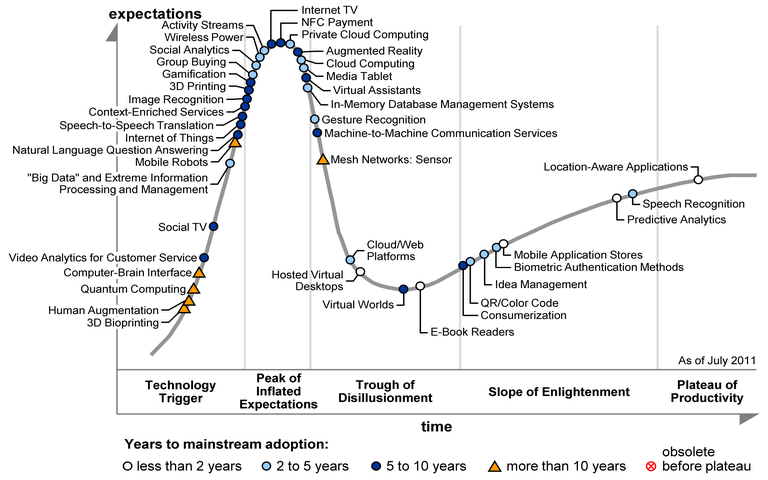
\includegraphics[width=0.75\textwidth]{gartner.png}
    \caption{Gartner Hype Cycle 2011 graphic}
    \label{fig:gart}
  \end{center}
\end{figure}

Despite being a term commonly referred, there is already criticism of gamification in the media. Some say that the term is a mere buzzword, applied as a simple "pointification", and often missing game elements such as storytelling and experiences, that are fundamental to the effectiveness of games.


\section{Existing work}

This section aims to introduce and analyse some existing services and applications related in some way to the concepts defined and explained in the previous sections of this chapter. This is particularly relevant because those concepts are behind the work meant to be developed in this thesis work and the project in which it is inserted.

\subsection{Social Networks for travellers}

In this chapter, it was already mentioned that there are 'themed' social networks, directed towards
people with particular interests or hobbies. 
There are also several online social networks aiming to promote the sharing of information between travellers. These platforms try to become a must see for those who are thinking of travelling, planning a particular trip, or want to find places to see in a particular journey or a comfortable place to spend the night during that journey.

Some examples of those platforms are \emph{WAYN} \footnote{\url{http://wayn.com}}, \emph{Tripatini} \footnote{\url{http://tripatini.com}}, \emph{Gogobot} \footnote{\url{http://gogobot.com}} and \emph{IgoUgo} \footnote{\url{http://igougo.com}}. They try to connect travellers and tour operators, using social networks.

\begin{figure}[h!]
  \begin{center}
    \leavevmode
    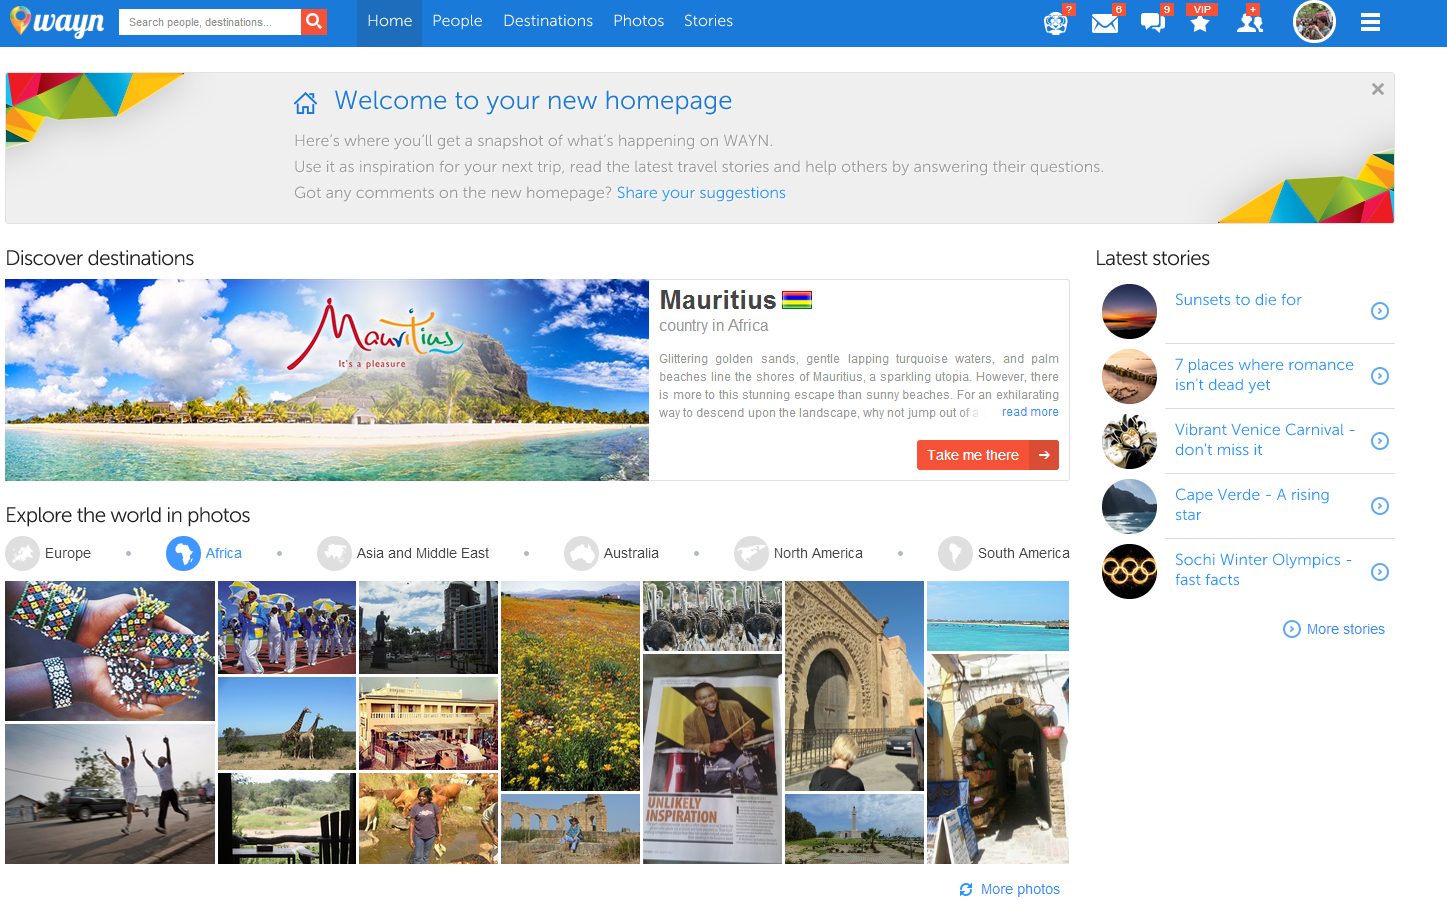
\includegraphics[scale=0.4]{wayn.png}
    \caption{Screenshot of \emph{WAYN} desktop interface}
    \label{fig:wayn}
  \end{center}
\end{figure}

However, these platforms have many disadvantages and do not represent what the implementation of the concept presented in \cite{kn:NGeCP11}. To start, these platforms aim to share information about long distance trips, in contrary to what is aimed to achieve (short-duration trips in a context of urban mobility).
Also, after a brief utilization and registration on some of those platforms, anyone can conclude that there is a strong presence of travel operators, filling up user's email accounts with messages, deals and offers to some destinations. 

A large percentage of the websites are also covered with those offers, turning the navigation and understanding of the platform very difficult and tiring, in what can be considered as a bad example of marketing utilization on online social networks, due to the excessive information that is presented.

Another problem of these platforms lies on the reliability of the information. In the end of 2009, a journalist named Arianne Cohen, tested the limits of these platforms by travelling to a foreign and unknown destination for her (in the particular case, Istambul), using only mobile applications and social media to receive information about places to see and where to spend the night. The resulting experience was disappoint in what concerns to these travel-themed platforms, as Arianne obtained most part of her positive experiences from contacting people through general-use platforms, such as \emph{Twitter}, \emph{Facebook} and \emph{Google+} \cite{kn:Coh10}.

\emph{Tripatini} presents us with yet another problem: usability and appearance. The platform's interface looks outdated and the existing information is not well-structured.

In addition to this social networks designed for travellers, some information about public transport can be found on general-use platforms, because public transport companies have realized about the potential the networks have to act as a way to get closer to their customers and daily users, communicating with them.
Nowadays, it is fairly common to find \emph{Facebook} and \emph{Twitter} pages from the companies, used to disseminate information about their services and interact more directly with the customers.
For instance, \emph{Metro do Porto} is present on both \emph{Facebook} \footnote{\url{http://www.facebook.com/MetroPorto?sk=wall}} and \emph{Twitter} \footnote{\url{https://twitter.com/\#!/metrodoporto}}, as well as \emph{STCP} \footnote{\url{http://www.facebook.com/STCPSA?sk=wall}} \footnote{\url{https://twitter.com/\#!/STCPServicos}}.

\subsection{Mobile Applications using Location-Based Services}

As said before, the increasing use of smartphones lead to the appearance of new and richer location-based services (concerning the amount of information they gather about users' location). Some successful online social networks based their business model or main features precisely on the capacity to track the location of their users.

Perhaps the most successful example of this kind is \emph{Foursquare} \footnote{\url{http://pt.foursquare.com/}}, who allows the 'check-in' of users at several locations (bars, restaurants, clubs, etc.), employing gamification techniques (badges) to improve user engagement with the network. The mobile application of the platform gathers the user location, giving him information about the nearest interest points, and allowing him to perform manual check-in at one of these locations.
A user earns a badge for completing tasks, such as checking-in for the first time at a new place, checking-in at a wide number of places in the same area, or several times in the same place. The platform also allows searching for particular categories of points of interest, and check the places visited by an user acquaintance.

\begin{figure}[h!]
  \begin{center}
    \leavevmode
    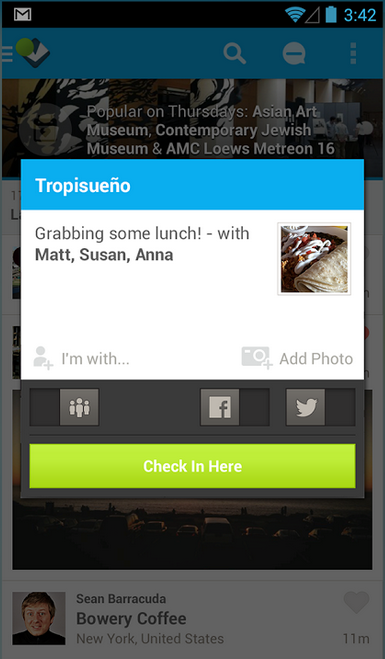
\includegraphics[scale=0.5]{foursquare.png}
    \caption{Screenshot of \emph{Foursquare} Android mobile application interface}
    \label{fig:fsqr}
  \end{center}
\end{figure}


\emph{Foursquare} had, as of February 2013, more than 40 million registered users, with several millions of check-ins registered in a daily basis.

Some other examples of successful online social networks that take advantage of the location of their users are \emph{Blendr} \footnote{\url{http://blendr.com/}} and \emph{Tinder} \footnote{\url{http://www.gotinder.com/}}. Their main goal is to, using that location, search for people nearby in order to arrange online dates between users.

\begin{figure}[h!]
  \begin{center}
    \leavevmode
    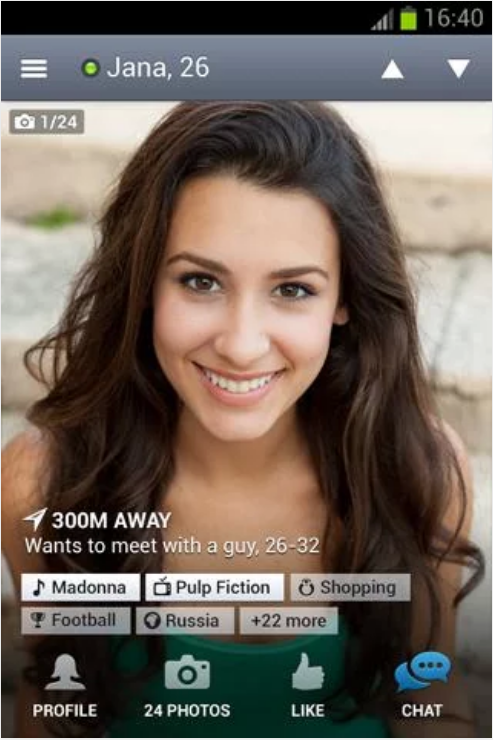
\includegraphics[scale=0.5]{blendr.png}
    \caption{Screenshot of \emph{Blendr} Android mobile application interface}
    \label{fig:blndr}
  \end{center}
\end{figure}

\emph{Tinder}, for instance, provides users with a sort of catalog from other users nearby, prompting them with a choice: marking them as a possible interest or not. Then, if the other person does the same thing, communication between the two users is enabled. 

\begin{figure}[h!]
  \begin{center}
    \leavevmode
    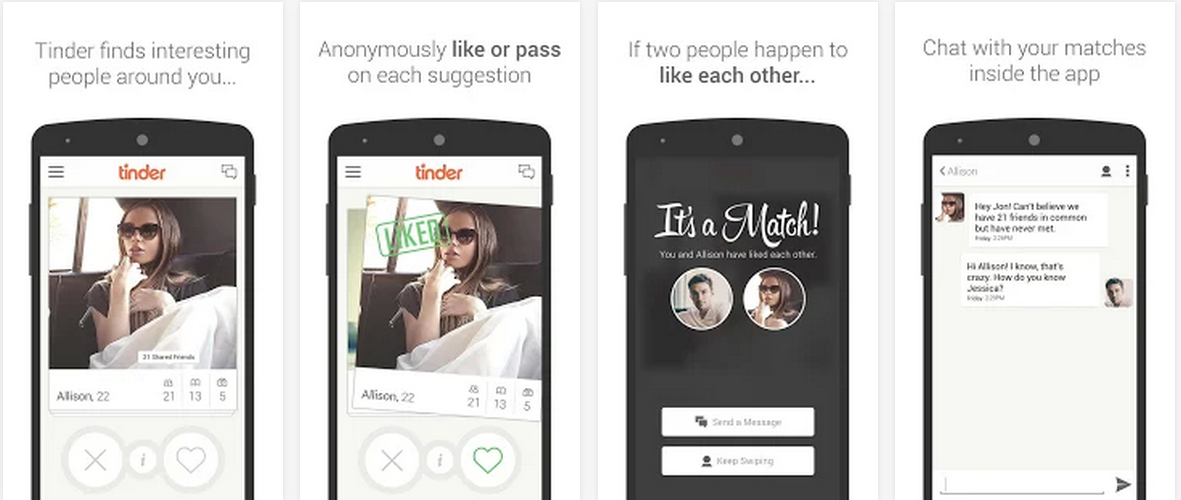
\includegraphics[width=0.8\textwidth]{tinder.png}
    \caption{Workflow of \emph{Tinder} application interface}
    \label{fig:tindr}
  \end{center}
\end{figure}

These two social networks, along with similar applications, demonstrate how a location-based service can be used in a context where the location of nearby users is deeply explored, and the number of existing users a critical factor for their success.

\pagebreak

\subsection{Route Planners}

Route planning services consist in one of the most used services for those who want to plan a trip using the Internet, whether it is short or medium duration trips. 
These services are usually free of charge, and allow their users to view Earth's maps and satellite images, offering route planning features using several types of transportation (walking, by public transport or by private car). They are particularly useful to find the shortest or fastest route between two given points. 
The most known service of this type is \emph{Google Maps}, but there are some alternatives, such as \emph{MapQuest} or \emph{Bing Maps}.

Given their features, these services normally have a simple and intuitive interface, making them easy to interact with.

\subsection{Mobile Applications for Public Transport}

In the last few years, some public transport companies tried to provide their users some valuable information about their services. That resulted in several applications, spread by a lot of countries and cities.

Some of those applications are: \emph{London Underground} \footnote{\url{https://play.google.com/store/apps/details?id=com.visualit.tubeLondonCity&hl=pt_PT}}, \emph{Catch that Bus!} \footnote{\url{https://play.google.com/store/apps/details?id=uk.co.ashtonbrsc.catchthatbus}}, \emph{National Rail Enquiries} \footnote{\url{https://play.google.com/store/apps/details?id=uk.co.nationalrail.google}}, \emph{iMetroPorto} \footnote{\url{https://play.google.com/store/apps/details?id=pt.edgelabs.metro_porto}} and \emph{MOVE-ME} \footnote{\url{https://play.google.com/store/apps/details?id=com.moveme}}.

\begin{figure}[h]
\begin{center}
\leavevmode
\subfloat[\emph{Catch That Bus!}]{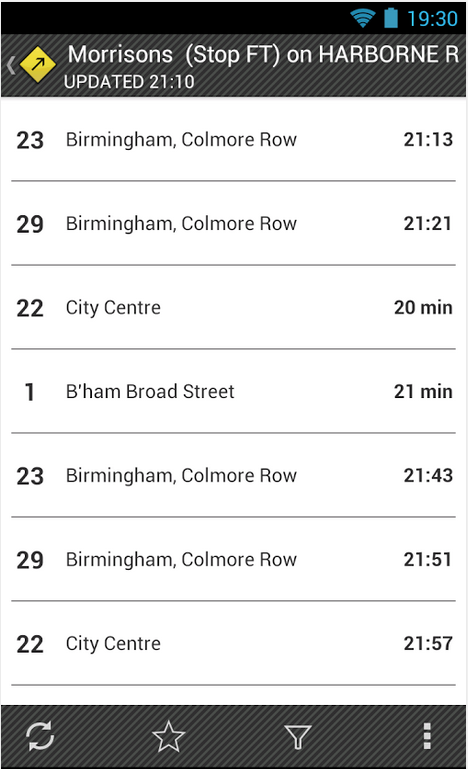
\includegraphics[width=2.5in]{catch.png}} \hspace{1em}%
\subfloat[\emph{London Underground}]{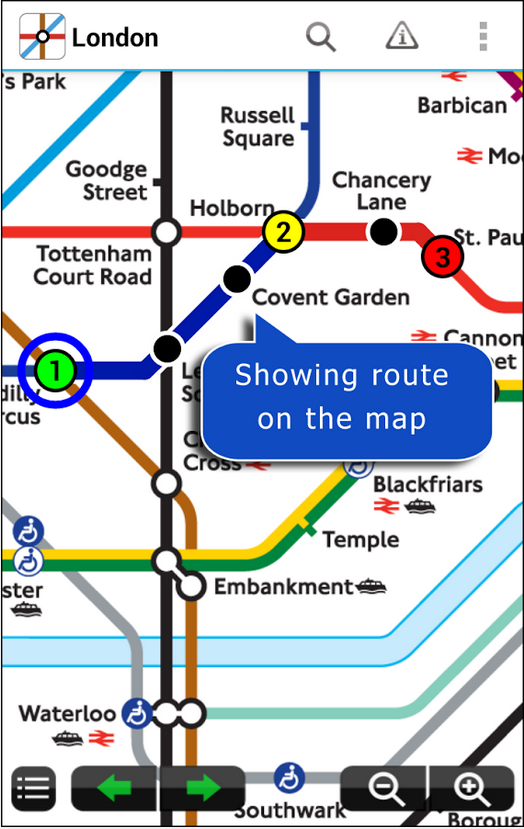
\includegraphics[width=2.5in]{london.png}}
\caption{Interfaces of mobile applications for public transport information - Example 1}
\label{fig:interfaces1}
\end{center}
\end{figure}

\begin{figure}[h]
\begin{center}
\leavevmode
\subfloat[\emph{National Rail Enquiries}]{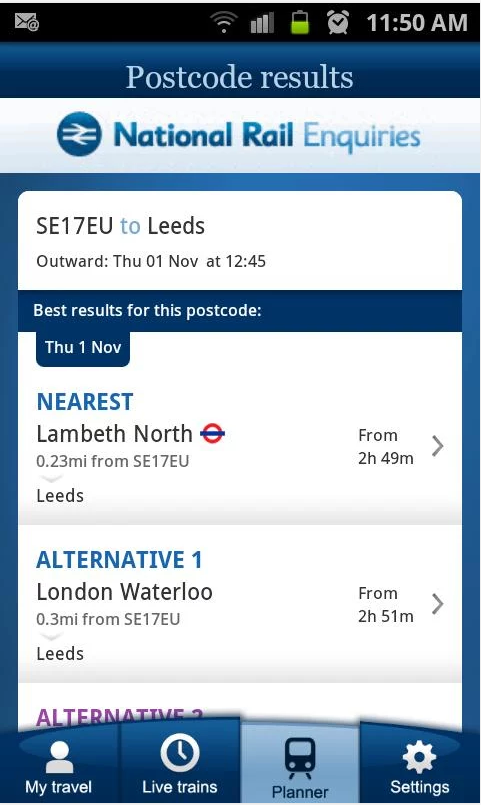
\includegraphics[width=2.5in]{national.png}} \hspace{1em}%
\subfloat[\emph{MOVE-ME}]{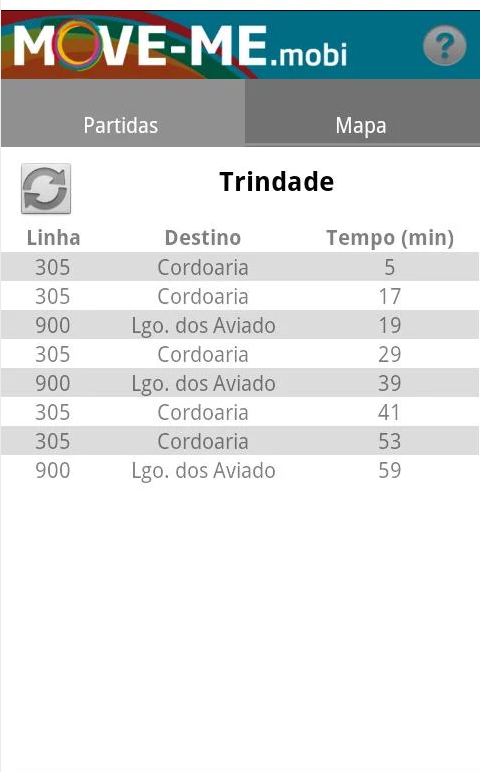
\includegraphics[width=2.5in]{moveme.png}}
\caption{Interfaces of mobile applications for public transport information - Example 2}
\label{fig:interfaces2}
\end{center}
\end{figure}



In the range of features provided by these applications, it is possible to find: 

\begin{itemize}
\item Information about schedules, lines and upcoming vehicles in real time.
\item Journey planner features.
\item Current location and nearest train/underground stations or bus stops.
\end{itemize}

There are, however, some disadvantages to this sort of mobile applications. They are usually limited to a city or urban area, or even to a specific method of transport, constraining their usage and potential.
The existing journey planner features, are in most cases pretty limited, not showing warnings or notifications to the users about delays or other events in the planned journey (only \emph{National Rail Enquiries} informs travellers about delays or cancelled trains).

Another downside of these applications, however not visible to the travellers, is that they rely on an existing API in the company's servers. To provide information of this kind to their clients, a public transport company must support the costs of developing and maintained such solution, costs that can be avoided if an application using crowdsourcing (where the information originates in the users themselves) is available in the said urban areas.

\subsection{Mobile Applications with Crowdsourcing}

Starting from the last constraint mentioned in the last set of existing applications, there has been developments in recent years in order to launch new solutions based on crowdsourcing, where users can access detailed information that were previously generated by other users. The potential of this type of applications is tremendous, specially in areas where there are many users  constantly using the application, receiving and submitting information possibly useful to other people with the same intentions. 
Obviously, transportation in urban areas is a field where this potential can be explored, giving the amount of people using private or public transport in a daily basis and sharing travel intentions.

That has lead to the appearance of platforms such as \emph{Tiramisu} \footnote{http://www.tiramisutransit.com/}, \emph{Waze} \footnote{\url{https://www.waze.com/}} and \emph{Moovit} \footnote{\url{http://www.moovitapp.com/}},  that are the closest existing applications compared to the project in which this thesis work is inserted.
\emph{Waze} is directed towards private transportation, feeding users with information about traffic and navigation provided by other users of the platform. Drivers can also report traffic issues, such as traffic jams or accidents, in order to warn other drivers, giving them the possibility to act accordingly with the situation.

\begin{figure}[h]
\begin{center}
\leavevmode
\subfloat[Route information]{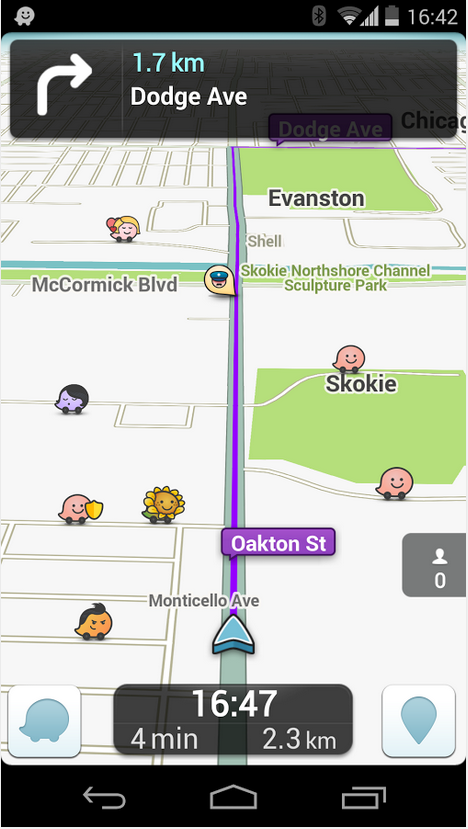
\includegraphics[width=2.5in]{waze1.png}} \hspace{1em}%
\subfloat[Report feature]{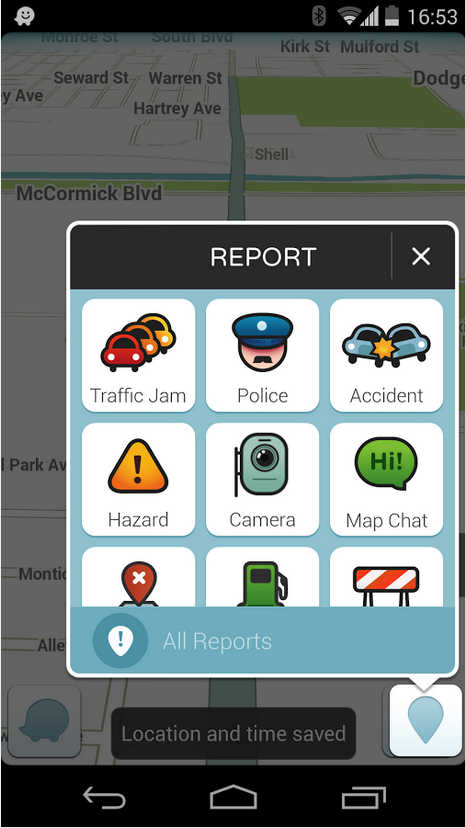
\includegraphics[width=2.5in]{waze2.png}}
\caption{Captions of \emph{Waze} mobile application interface.}
\label{fig:waze}
\end{center}
\end{figure}

\emph{Moovit}, however, is directed towards public transportation, feeding users with information about schedules in real time, re-routing in case of  delays, and also about crowding level of the vehicle.
The information provided is generated by and shared between other users, thus making \emph{Moovit} the most similar platform to this project's concept (however, it still does not take into account other aspects of the trip that we aim to see shared between users).

\emph{Moovit} is available in several countries and cities all across the world, with relative success. 
In Portugal, however, it is not available yet. As of 8th of June 2014, the mapping of the public transport lines and schedules for the city of Porto was started by the community, but the lack of users acts as a constraint to the availability of the application for this city's public transport users (still plenty of work to be done in that field), and to its success (with few users, most of the lines would not have information at all, even during the day, because all the information in this application is supplied by its users). 

\begin{figure}[h]
\begin{center}
\leavevmode
\subfloat[\emph{Trip information feature.}]{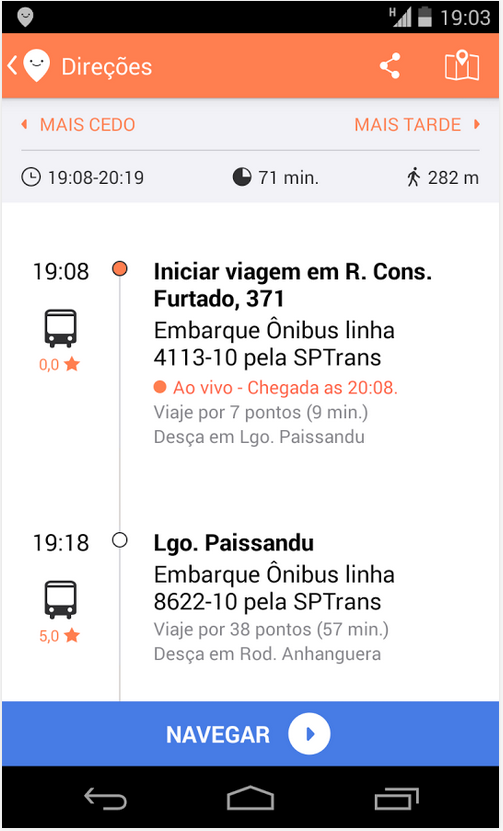
\includegraphics[width=2.5in]{moovit1.png}} \hspace{1em}%
\subfloat[\emph{Report information feature.}]{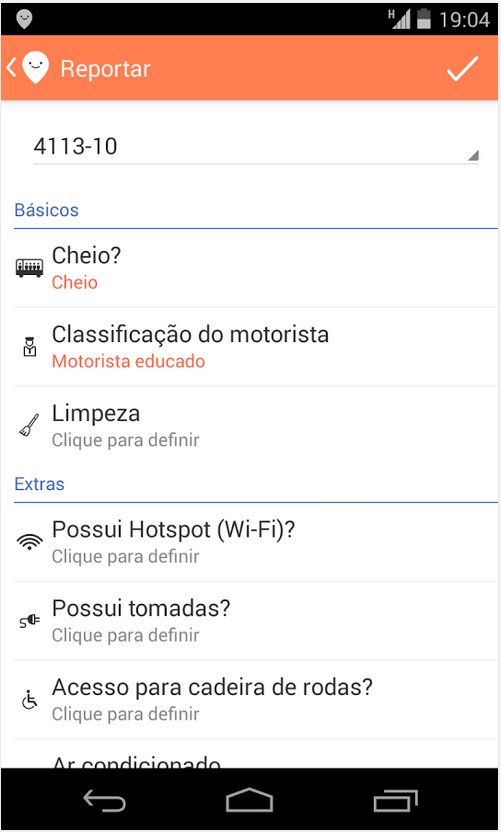
\includegraphics[width=2.5in]{moovit2.png}}
\caption{Captions of \emph{Moovit} mobile application interface.}
\label{fig:moovit}
\end{center}
\end{figure}

\emph{Tiramisu} is also directed towards public transportation, being focused only on buses. However, it takes advantage from the users GPS location (during a bus trip) in order to predict the bus arrival time and present it to other users. In addition, a user travelling on a bus can report to the application if the bus is full or if there are seats left. 

For buses that have no users of the application inside (thus, not recording their location), the application displays the official schedule from the transport operator (not in real time, but the same as the printed scheduled arrive time). \emph{Tiramisu} is only available for a few number of cities and operators in the United States of America.


A final note about the interface of \emph{Waze} and \emph{Moovit}:  after a brief use, the interfaces seemed very attractive, but not exactly clear to the user in what the buttons in the interface are meant to do or show.

\section{Summary}

After the literature review and a study of existing applications, it is concluded that there are good examples of services that use location of users and gamification techniques to improve user engagement, and that some of those aspects can be used in the interface meant to be developed in this thesis work. 

Concerning applications directed for public transport information, besides the limitations already mentioned, there are no applications feeding users with the information this project desires to provide them with. Also, because the final desired prototype is not limited to show information to the users, but also to make the task of sharing and submitting information as simple as possible, the usability of the application gains much more importance compared to the other existing applications in the field.
\chapter{Problem Description and Approach}\label{chap:chap3}

\section*{}

As described in the section \ref{sec:goals} of the introduction, the project encompasses the creation of a functional prototype for an \emph{Android} mobile application for a platform that uses dynamic social networks and intends to use gamification techniques to improve user engagement. The platform is designed to share information about public transport between travellers.
Before the implementation of the functional prototype, the creation and testing of interface designs is required. 
The usability and interaction of that interface is fundamental to the platform, because it might make the difference between its success or failure, given that it might attract or repel several users and facilitate or make more difficult the submission of information through the platform.

According to a study performed by Robert Pessagno \cite{kn:Pes10}, "[social networks] acceptance is determined by how easy it is to use them", and that has even more importance in the scope of this project, given the necessity of having a large base of users feeding the platform with a huge volume of information in real time at any given moment. If that does not happen, there is a risk of having lines with no information. For instance, low transport frequency time periods or low frequency lines may lead to inexistent information in those lines or during those periods. Having a greater user base mitigates that risk, though it can still happen.

Given the innovation introduced by the main feature of the project, the dynamic social networks, it is necessary to develop suitable metaphors and create user visual affordance to enable the understanding of that feature by travellers, in a familiar or intuitive way for them.
In the first iteration of the project \cite{kn:eSG12}, usability tests were performed in order to capture possible usability problems with the previously developed interface (Figure \ref{fig:current}). 
Those tests resulted in a set of conclusions that encompassed  usability issues to be addressed and aspects to improve in this new iteration, and it is aimed to use those conclusions as a starting point to this work (see \ref{sec:initial}). 

\begin{figure}[h]
\begin{center}
\leavevmode
\subfloat[\emph{Trip information feature.}]{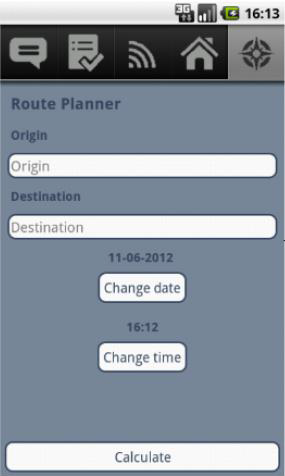
\includegraphics[width=1.7in]{current1.png}} \hspace{1em}%
\subfloat[\emph{Report information feature.}]{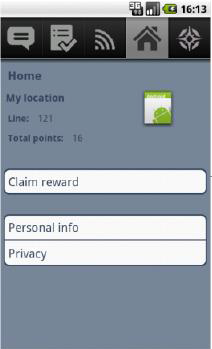
\includegraphics[width=1.7in]{current2.png}}
\subfloat[\emph{Trip information feature.}]{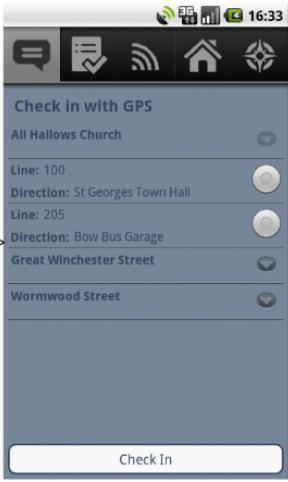
\includegraphics[width=1.7in]{current3.png}}
\caption{Screenshots of the previously implemented interface.}

\label{fig:current}
\end{center}
\end{figure}

\pagebreak

\section{Usability}

Usability can be defined as a measurement for how easy it is to use an interface. Typically, the evaluation or measurement of usability is kept separate from discussions of utility, a characteristic often more influenced by what the interface is connected to (if we're talking about a mobile application, that can be for instance an existing API retrieving data existing in an external server) than the interface itself. 
Jakob Nielsen, one of the most prominent authors and experts on usability, defines usability as having the following components \cite{kn:Nie12}

\begin{itemize}
\item \textbf{Learnability} - How easy it is to users to accomplish basic tasks in the first time they are introduced to the design?
\item \textbf{Efficiency} - Once the users have passed the learning phase, how quickly can they perform tasks?
\item \textbf{Memorability} - After a period of not using the interface, how quickly can users remember it and be proficient in the accomplishment of tasks?
\item \textbf{Errors} - How many errors do the users make while using the interface? What is the severity of those errors and can they recover from them?
\item \textbf{Satisfaction} - How pleasant is it to use the design?
\end{itemize}

Following Nielsen's approach, only actual performance by users is worth measuring. However, there are other approaches, for instance the one defined by Patrick Jordan, that include the theoretical performance level achieved when the system being measured is used to its full potential \cite{kn:Jor94}.

Despite the several definitions and approaches, the goal of  (improving) usability, that aims to be accomplished in this thesis work, is to make it faster and easier to users of an interface to achieve their goals and accomplish the desired tasks.


\section{User-Centered Design}

In the recent years, the attempt of several institutions to integrate design with technology has become a regular behaviour in the development of their products.
In 1999, it was established an international standard, \emph{ISO 13407}, that aimed to provide "guidance on achieving quality in use by incorporating user-centered design activities throughout the life cycle of interactive computer-based systems."

That standard established four activities that had to be started at the earlier stages of a project:

\begin{itemize}
\item Understand and specify the context of use for the product - Collect relevant contextual information from the environment where the system is going to be used;
\item Specify the user and organisational requirements - Formulate and build the user-centered
requirements for the new software.
\item Produce design solutions - Simulate design solutions using paper or computer-based mockups and get feedback of real users;
\item Evaluate designs against requirements. Last but not least,is indispensable to evaluate
the design work performed previously. In this phase anomalies, defects, bugs, failures are detected in order to select the best solution for the system.
\end{itemize}

These activities were meant to be performed according to the workflow presented in Figure \ref{fig:iso}. This standard has since then been revised and re-issued as \emph{ISO 9241-210}, which describes six key principles to apply in a user-centered design process \cite{kn:Tra11}:

\begin{figure}[h!]
  \begin{center}
    \leavevmode
    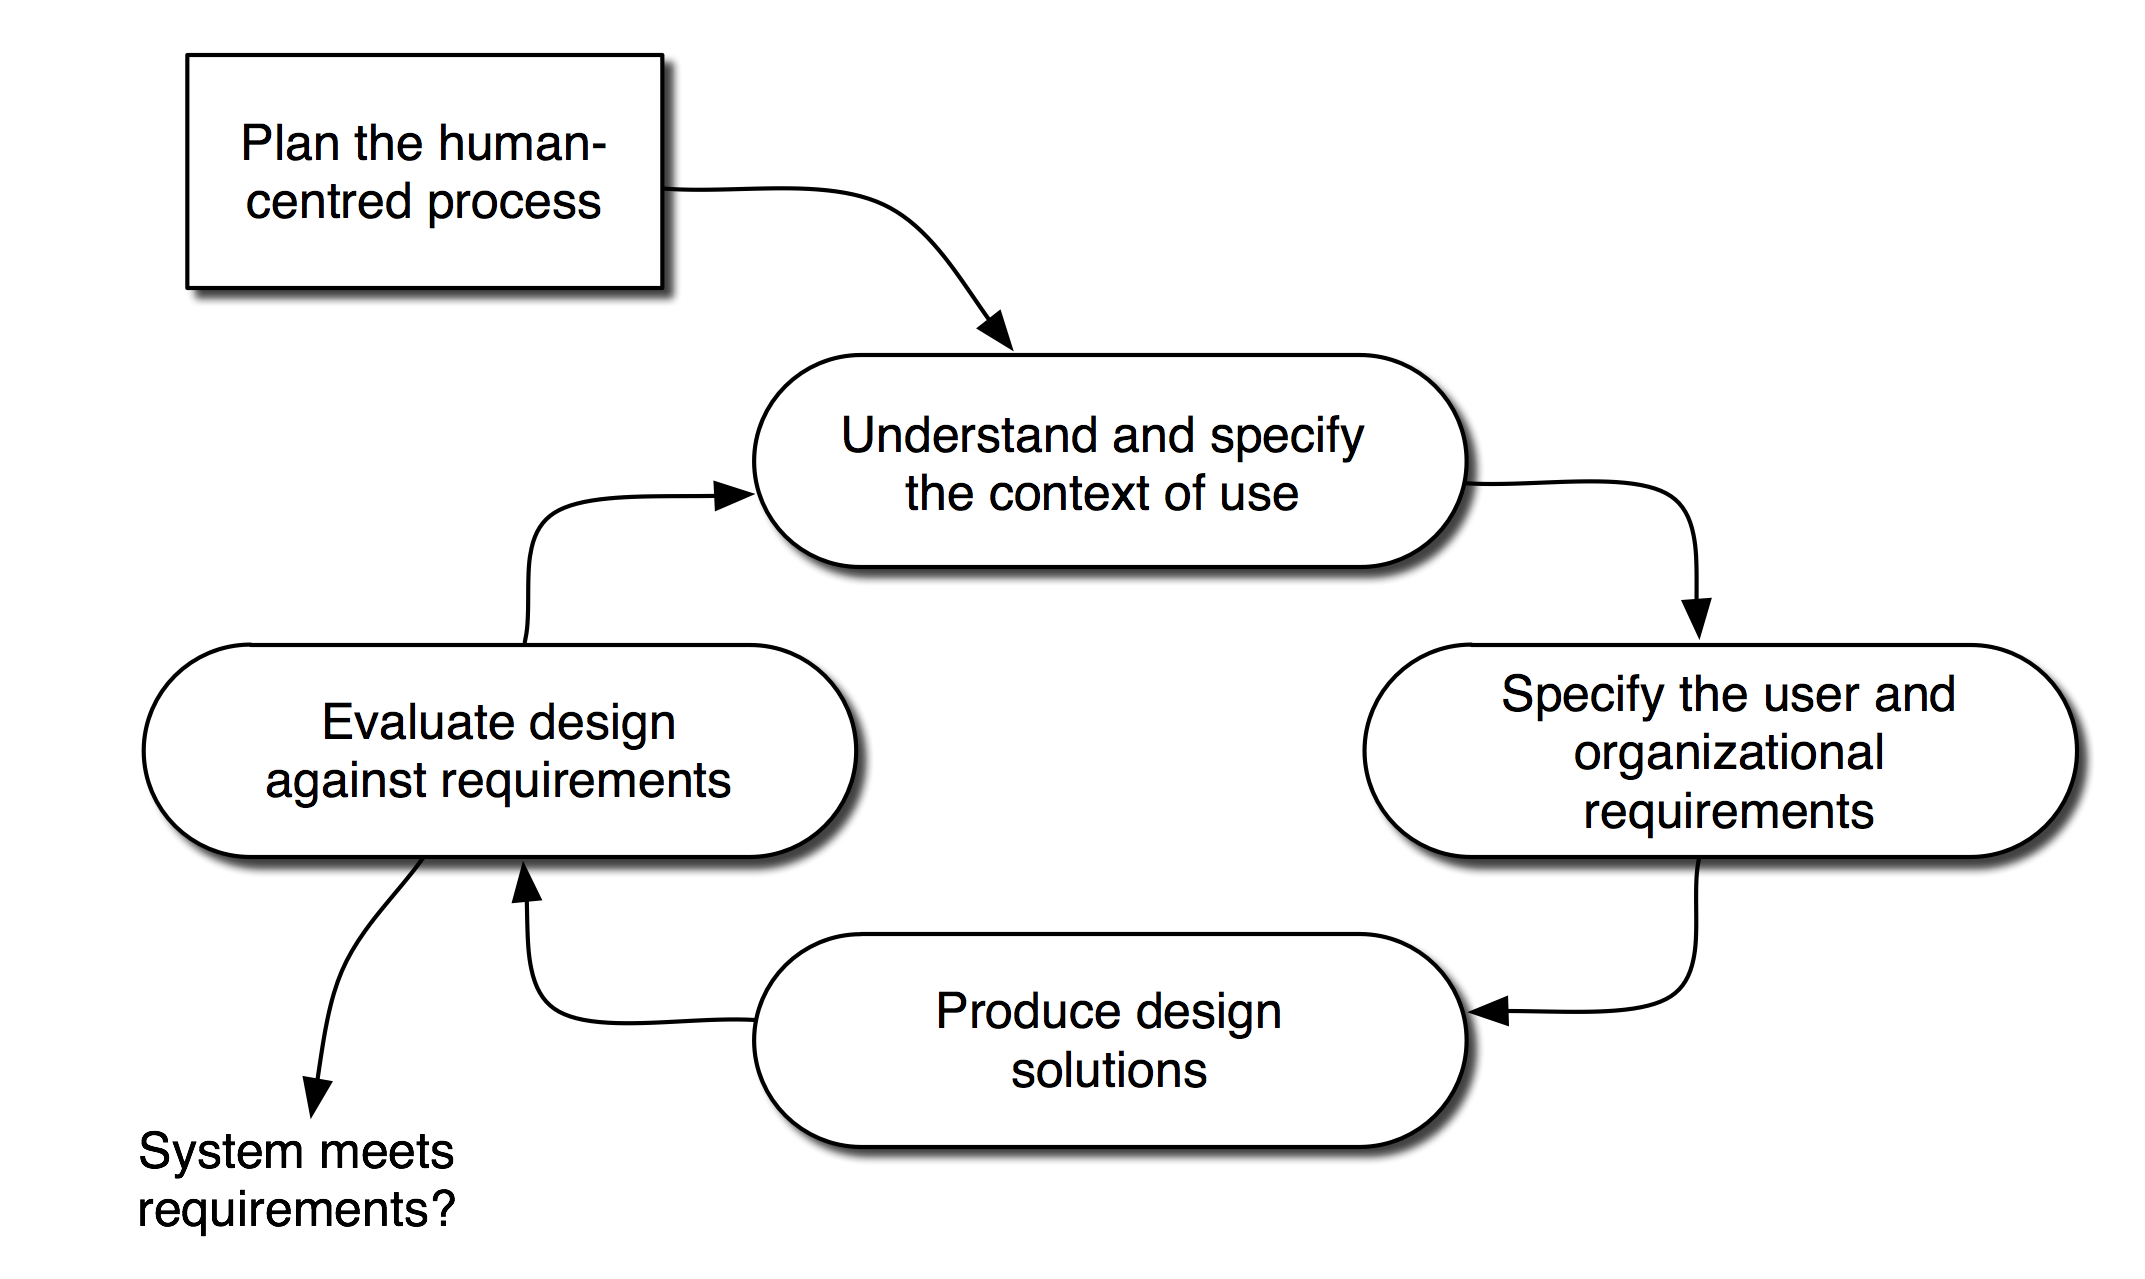
\includegraphics[scale=0.8]{iso13407.png}
    \caption{Workflow of the process described in \emph{ISO 13407}.}
    \label{fig:iso}
  \end{center}
\end{figure}

\begin{itemize}
\item The design is based upon an explicit understanding of users, tasks and environments. This means that is necessary to understand your users, understand what they want to do with the system and understand the environment in which the system is used.

\item Users are involved throughout design and development - Users must be involved in all design phases, not just at the start and at the end of the design.

\item The design is driven and refined by user-centered evaluation - Usability testing should be carried out throughout the design process. Initially, to test preliminary designs such as paper prototypes, and after that, not just at the end of the process.

\item The process is iterative - It is difficult, if not impossible, for users to explain what they want or need from a system. So, in order to find out what people want, it is necessary to show them something that they probably don't want (first designs) and then discover how to improve it. This means that if a waterfall methodology is used the design process will struggle to be user-centered.

\item The design addresses the whole user experience - Usability (and a good user experience) is about a lot more than making things simple, including the perceptual and emotional aspects typically associated with user experience.

\item The design team includes multidisciplinary skills and perspectives - The design team should include a range of views, including the voices of accessibility experts, end users, domain experts, etc.
\end{itemize}



Given those recommendations and the referred importance of making the users part of the development process (thus increasing the chance of success of the application among a wider audience), the chosen process in order to achieve the expected results has four phases: 

\begin{itemize}
\item \textbf{Requirements Elicitation phase} - As an initial step, it should include an analysis of what went wrong or what were the perceived disadvantages in the interface previously conceived, followed by additional usability requirements elicitation (assembling a focus group with potential users of the application and regular public transport users);
\item \textbf{Design phase} - Consists in the creation of alternative low-level designs, along with the usability tests and studies in order to maximize their quality and relevance.
\item \textbf{Prototyping phase} - Implementation of a chosen design, previously done, as an \emph{Android} mobile application.
\item \textbf{Evaluation phase} - Realization of usability evaluation and analysis of the evaluation results, as the name suggests.
\end{itemize}

It is worth referring that this process is an adaptation encompassing the iterative process described in \emph{ISO 13407}, where the mentioned Requirements Elicitation phase serves as the first iteration that allows the gathering of a vast amount of information regarding usability requirements, that will result in the production of an initial design, that will be checked against additional requirements.

The following design phase will act as several iterations of the process, constantly evolving the interface and trying to improve the quality of the solution. That phase will end with a usability test with potential users, that will serve as validation of the evolved design in order to pass to the implementation phase.

Finally, the implementation and evaluation phases will act as a final (and long duration, due to the duration of the implementation) iteration of the process. 

\subsection{Usability Evaluation}

The usual approaches to perform usability evaluation are the following:

\begin{enumerate}
\item \textbf{Usability testing} - Involves measuring typical user's performance on task accomplishment.
\item \textbf{Field studies} - Performed in a natural environment (real case scenario)
\item \textbf{Analytical evaluation} - Does not involve end-users. Two main methods are usually used, heuristic evaluation and/or predictive evaluation. While heuristic evaluation involves the use heuristics (sets of guidelines and standards) and walkthroughs with experts through scenarios of the application prototypes, predictive evaluation is based on theoretical models, in order to predict user performance.
\end{enumerate}

Heuristic evaluation with experts will be employed in a final phase, to evaluate the functional prototype and to validate the implemented interface, serving as a base to possible future improvements.

\subsection{Usability Tests}

In order to measure and improve usability of a given project, usability tests are often performed. An usability test serves as an important tool for the usability evaluation of an User Interface, in which the effectiveness of the User Interface itself is analysed. Based on the results of that evaluation, changes can be made to improve the interface and the interaction of the said project.

These tests often consist in observing users accomplishing a given set of tasks in the application, or even looking at a User Interface and checking it against common design rules and guidelines \cite{kn:Joh14} and identifying the origin of possible unexpected/unwanted behaviours in its utilization.

The process of performing the usability test includes the definition of what is meant to be evaluated, the choice of participants for the test, the creation of test tasks and scenarios, and the selection of evaluation metrics aligned with the goals defined for the test.

In the scope of this project, usability tests are necessary to include users in the evolution process of the designed interface, and also to present a validation method to that interface before an implementation phase. These tests will be performed through the design phase, promoting the correction and improvement of the designed interface, recurring to potential user observation and questioning.




\chapter{Requirements Elicitation}\label{chap:chap4}

\section*{}

This chapter will present in detail the first stage on the development process of this thesis, covering the initial usability requirements elicitation.

The following sections provide an analysis of the previously existing work on the project and conclusions drawn from that work, as well as the process that lead to a first redesign, based on those conclusions.

In the last section, the referred redesign, consisting in several alternative solutions, will act as a discussion material in a focus group performed with potential users of the application, in order to elicit usability requirements. All the process of the focus group, as well as all the data gathered from it, is detailed there.

\section{Previous work}

As said before, the initial work on this project encompassed the initial implementation of the concept referred on \cite{kn:NGeCP11}, including a first prototype of an \emph{Android} mobile application. This prototype was made using \emph{Android} API level 8, being compatible with mobile devices running at least version 2.2 of the operative system.

This prototype had the following set of features \cite{kn:eSG12}

\begin{itemize}
\item Login
\item Register Account
\item Check-in
\item Check-out
\item See News Feed
\item Submit a Comment
\item Rate a Comment from Other User
\item Plan a Journey
\end{itemize}

A more detailed explanation of those features, introducing some of the interaction flow of the prototype, is the following:

\begin{enumerate}
\item User launches the application, being prompted to login or to register a new account if he had not created one yet. If the user does not have an account, he has to register and is guided to the login screen.

\item User has the possibility to check-in on a vehicle by two methods: manual insertion of the public transport stop names (origin and destination), or by GPS, where the user location is used in order to fetch the nearest stops, marking a chosen one as the origin, and choosing the destination from one of the given possibilities, thus marking the journey is making at that given moment.

\item While checked-in (\emph{and only then}) the user could perform actions like submit a new comment for the selected journey (that could be written text comment, to a maximum of 150 characters, or a predefined categorised comment, rating aspects of the vehicle or driver, which was converted to text afterwards), check a news feed with comments from other users made for the same journey, and rate the correctness of comments from other users.

\item User could also perform check-out, in order to mark the end of the journey.

\item User could check his/her profile in order to check their number of points (awarded from submitted comments) and change settings like his nickname or if that nickname will be hidden from other users (in their news feed).

\item Finally, users could plan a journey for the future, setting the origin and destination stops, and choosing a date and time. Ten minutes before the planned journey, the user receives a notification asking if he wants to receive information for that journey (thus checking-in on the journey).
 
\end{enumerate}

The developed prototype was the subject of a test in the field, performed in London with real bus users. A certain number of tasks, exploring all the features above mentioned, were given to the users, in order to measure the average execution time of each task \cite{kn:NGG13}.

Despite the obtained results (average times for task completion were considered positive), there were tasks that could or should have better accomplishment times, given their importance in the whole user experience and utility.
For instance, planning a journey takes more than 80 seconds, on average (despite being referred that happens due to a bug in a auto-complete feature), but there are a lot more features taking more than 30 seconds on average to be accomplished (check-in in, whether through the manual method or using GPS location, and rating a comment from other user). 

Regarding the check-in functionalities, this can be a problem since it is a feature used on a critical part of the application - check-in is required to access several other main use cases. Making this process too extensive or making those features only accessible to checked-in users may lead to loss of interest by potential users.

One of the possible causes to this unwanted results is the fact that the check-in options are not accessible at a user's view level after logging in with his account - in order to perform check-in, users had to press the \emph{Android} Menu button (which prompts up the context menu to the user, where they would find those options).

The same principle is valid for the check-out feature, as the button who triggers it is also found in the context menu. 

Despite the results obtained for this task were much better, that is probably due to the fact that, in order to perform check-out, an user has to check-in in the first place, learning the place where the check-out button is when he's faced with the check-in task.

Still, no visual element whatsoever gives the user the information that the context menu is available to be shown. We should not rely on previous experience that the final user may have with the platform/operative system for which we are designing an interface, specially if that possible experience includes gestures, buttons or other interaction triggers that may be unfamiliar for the user in similar contexts or not visible.

There was another task with average accomplishment time exceeding 30 seconds - submitting a written comment - though it's fair to assume that most of that time consists in writing the desired comment, and it is not necessarily tied to a disadvantage of the interface.

Another measurement taken was a quantitative value (from one to five) representing the appraisal of a given task, concerning its difficulty, so that one represents a very difficult task to execute, and five represents an easy task.
Here, the tasks that could have had better results were related to the notification system (informing a user that he has a planned journey soon, asking if he wants to receive information from it and check-in), as well as rating other users comments (Figure \ref{fig:rate_tab}). 

This last concept was perceived as difficult to grasp, suggesting that improvement on this feature or the whole comment validation system, in order to provide more reliable feedback to public transport operators, can and should be made.
The less positive appraisal from the rating comment task could also be associated with the fact that this feature has his own tab (the main navigation is composed by tabs), thus getting less visibility when comparing to other tabs (news feed or comment tab, for instance). 

A possible solution to this problem could consist in aggregating both the news feed and rate separators, giving this feature more visibility, because one of the goals of the application is to maximize the reliability of the generated information. Thus, having as much users as possible performing ratings (by simplifying that task or the interaction behind it, or by augmenting its visibility) is crucial.

\begin{figure}[h!]
  \begin{center}
    \leavevmode
    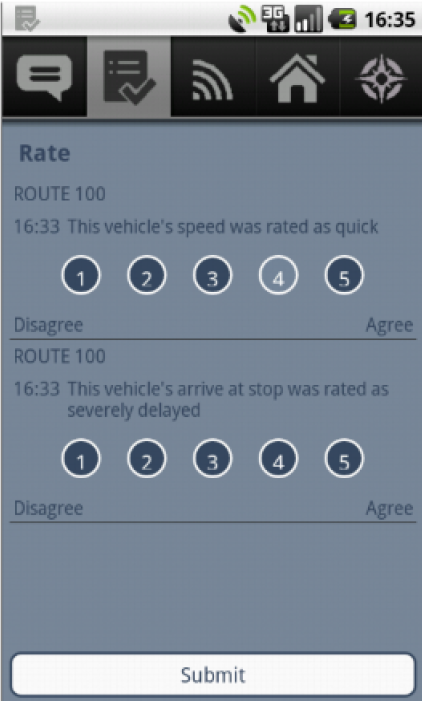
\includegraphics[scale=0.6]{rate_tab.png}
    \caption{Screenshot of the tab where we could find the rate comment feature.}
    \label{fig:rate_tab}
  \end{center}
\end{figure}

\pagebreak

All these questions and conclusions led to the development of a initial interface redesign, presented in the following section.

\section{Initial Proposals}\label{sec:initial}

After the initial process of perceiving what was done before, as well as understanding what were the advantages and disadvantages of the previous design decisions, and what went well and could go better, there were five groups of research questions to be answered in order to proceed with the next steps. Those questions were:

\begin{itemize}
\item Technology - Despite being still on a premature phase, what technology would be used in order to develop the functional prototype? In this case, since that prototype is expected to be an \emph{Android} application, what would be the versions targeted for the prototype?

\item Main Navigation - How to design the main navigation for the application? Stick by the use of the tabs? Explore other solutions used in similar contexts? 

\item Information shown on User Profile - What is relevant to be shown to the user? Does the user wants to see nearby users? Is he willing to allow his location to be shared and to see where are the users generating useful information to them? Or does he want to focus on more personal information, such as possible rewards, points, statistics and so on?

\item Comment, Rate and News Feed features - Can these be aggregated in a way user understands or is familiar with, or it represents an excessive amount of information to be shown in one screen? 

\item Journey Planner features - Could other features with perceived utility to the user be added in order to allow a better comprehension of the concept behind the application, and consequently, a more efficient use (for instance, saving time and avoiding repetitive tasks)?
\end{itemize}

\subsection{Technology}\label{technology}
Some thought should be put on the first mentioned topic from the beginning, since the target version of the future application, apart from the possible conditioning of target users (who have outdated \emph{Android} versions on their devices), can influence the implemented interaction, since the newer versions of the operative system have several features related to animations, UI styling and interaction patterns.

The main decision was between sticking with a target version of \emph{Android} 2.x (however, using the API for version 2.3.3 instead of 2.2, because as of February 2014, \emph{Android} 2.2 users represented about only 1\% of all the \emph{Android} devices worldwide) or developing the prototype only for versions equal or superior to 4.0.3 (\emph{Ice Cream Sandwich)} \cite{kn:Goo14}. 

Despite the fact that the users of \emph{Android} versions inferior to 4.0.3 represent about 15\% of total \emph{Android} users, that number will surely reduce with the emergence of newer versions and devices. The 'time to market' of the application is expected to be wide, though, so it is expected that, when a fully implemented and improved version of the project is ready to be launched, those 15\% don't pose a limitation anymore. Apart from that fact, the advantage of developing the application for versions equal or superior to 4.0.3 is huge, because the API versions between \emph{Android} 3.0 and 4.0.3 introduced major improvements to the UI, text input and so on. 

Another important feature of this version is the Action Bar, used in the majority of \emph{Android} applications in order to serve as the main navigation menu of those applications, and that could be used as well in this project. The Action Bar menu came as a replacement for the Context Menu in older versions of \emph{Android} (see Figure \ref{fig:action}).

\clearpage

\begin{figure}[h!]
  \begin{center}
    \leavevmode
    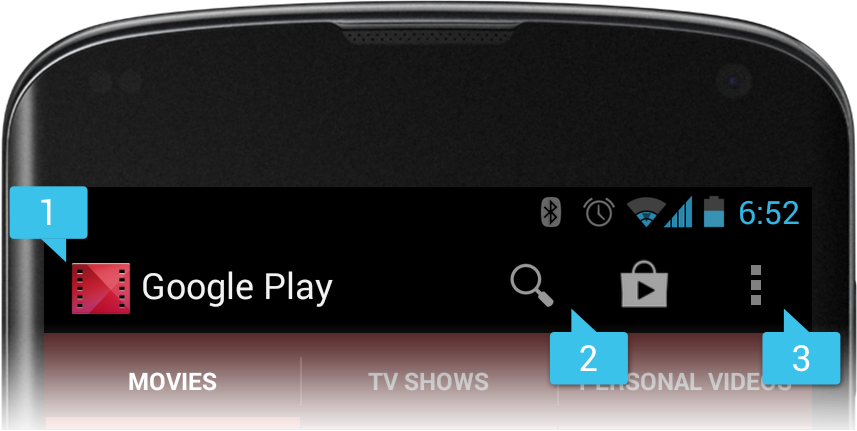
\includegraphics[scale=0.2]{actionbar.png}
    \caption{Example of an Action Bar from an \emph{Android} application, displaying the application icon (1), action items (2) and a menu option (3).}
    \label{fig:action}
  \end{center}
\end{figure}

It is also worth mentioning that one of the reasons of that change is the tendency to eliminate physical buttons from mobile devices (the first devices with \emph{Android} 4.0.3, such as \emph{Samsung Galaxy S III}, only had one physical button beneath the screen, resembling what happens with \emph{iOS} devices, and newer devices don't have a physical button beneath the screen at all).  

\subsection{Main Navigation}

About the main application navigation, the initial decision was to stick with a tab navigation, where a tab provided the access to one of the major features or modules of the application. However, there were several other questions that could be relevant:

\begin{itemize}
\item \emph{Screen position} - Top or bottom. Because we're talking about an \emph{Android} application, the best position would be top of the screen, since the recent versions of \emph{Android}, because of the already mentioned attempts to eliminate physical buttons on the devices, now has a bar on the bottom which has three buttons - \textbf{Back}, \textbf{Home} and \textbf{Recents} (this last one showing recently opened applications.

To put the tab navigation component could lead to user mistakes (touching the mentioned bar instead of the tab navigation). A tab navigation component in the bottom of the screen is, however, pretty common in \emph{iOS} mobile applications. 
There are a few cases where a navigation bar is placed in the bottom of the screen on \emph{Android}. For instance, when using the Action Bar for navigation, if there are a wide number of options that is desired to show to the user, it is possible to split the Action Bar, having the (usual) top one and another bar at the bottom (Figure \ref{fig:evernote}). 


\end{itemize}

\begin{figure}[h!]
  \begin{center}
    \leavevmode
    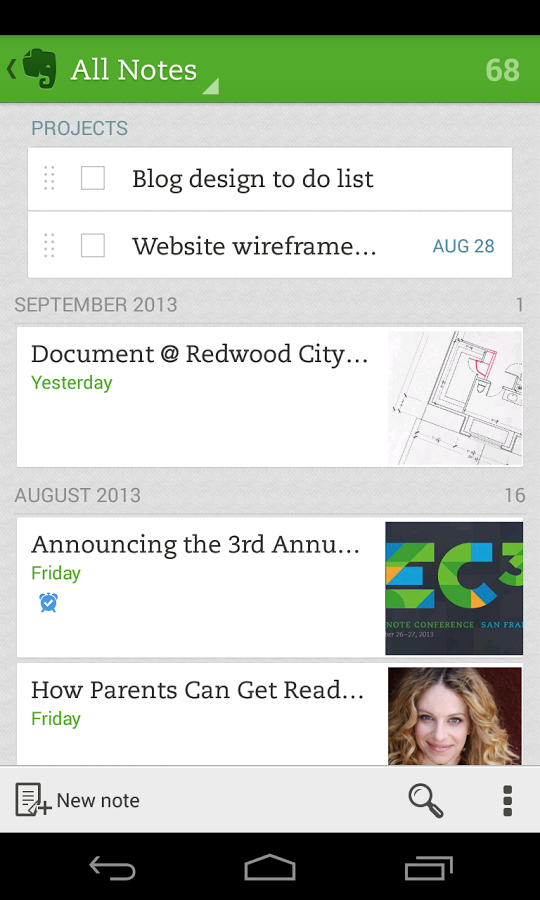
\includegraphics[scale=0.5]{evernote.png}
    \caption{Example of an application with splitted Action Bar - Evernote. Note also the bottom bar, present in recent devices.}
    \label{fig:evernote}
  \end{center}
\end{figure}

\begin{itemize}
\item \emph{Number of Tabs} - This number would depend on several factors. Visibility to the user is one of them. To have too many tabs, where some of them are initially hidden to the user (just accessible by using the swipe gesture, for instance) may cause those tabs and consequently the features they provide to be 'forgotten' and not as used as intended. 

In the work mentioned in the previous section, there were five tabs, all immediately visible to the user. This was perceived as an high number of tabs shown to the user. Reducing the number of visible (or total) tabs to three or four was explored in order to produce new design solutions.

\item \emph{Information displayed} - The previous prototype had icons representing each tab. There were no text labels displayed, and none of these icons is familiar to the user from similar contexts (applications or websites usage), apart from the icon from the fourth tab, intended to represent the tab containing the user profile. 

Metaphors that users associate with well-defined actions, pages, features or contexts, should not be used in order to represent different actions or contexts, because that will only confuse the user, improving the possibility of errors and confusion by the user. The biggest example of this is the 'save button'. An icon with a 3.5" floppy disk has been used for decades and has spread as representing the "save" action in a certain application. Today, despite the fact the younger generations don't recognise what a floppy disk is, they still associate the icon with saving.

In this case, the icon for the user profile tab as a house, usually associated with the existence of an Home screen or page. However, what was considered the 'Home tab' was in fact the user profile and not the start point of the application, and this issue could lead to errors or confusions from the user point of view.
\end{itemize}

Considering these points, two alternative designs were conceived for this component (meant to be discussed on a focus group session), all with four tabs - one with only three tabs visible at a given moment (the selected one should have a visible indicator in order to inform the user from that status), with no icons and just text labels (Figure \ref{fig:tabs1}); one with four fixed tabs (all visible), containing both icons and text labels (Figure \ref{fig:tabs2}). A slight variation of this one was also designed - with the addition of a coloured circle indicator to show the number of new items on the news feed list (Figure \ref{fig:tabs3}).

\begin{figure}[h!]
  \begin{center}
    \leavevmode
    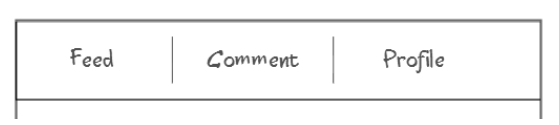
\includegraphics[scale=0.8]{tabs1.png}
    \caption{Initial draft of the tab component - three visible tabs, only text labels.}
    \label{fig:tabs1}
  \end{center}
\end{figure}

\begin{figure}[h!]
  \begin{center}
    \leavevmode
    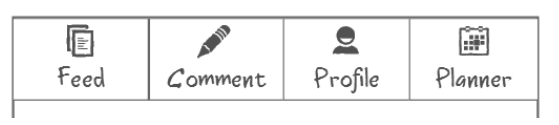
\includegraphics[scale=0.8]{tabs2.png}
    \caption{Initial draft of the tab component - four tabs, icons and text labels.}
    \label{fig:tabs2}
  \end{center}
\end{figure}

\begin{figure}[h!]
  \begin{center}
    \leavevmode
    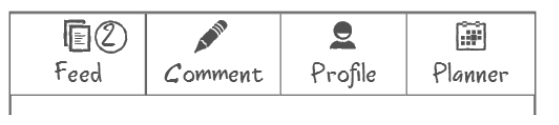
\includegraphics[scale=0.8]{tabs3.png}
    \caption{Initial draft of the tab component - four tabs, icons and text labels, and coloured indicator.}
    \label{fig:tabs3}
  \end{center}
\end{figure}

\subsection{User Profile}

The previous prototype gave the user the chance to check their points, stars and their username on their user profile, as well as change their nickname and a setting that allowed them to hide their nickname to other users. 

An additional button was also available, meant to fetch possible rewards that users could claim using points. Considering this, the displayed information was insufficient, too much free space remained vacant, and that space could be used in order to display other information the users of the application could find useful.

After an initial brainstorming session, there were several ideas about what sort of information could be displayed - user photo/avatar, a map of users in the same temporary network of the user (users who could contribute to the news feed that the user is receiving), information about the line and vehicle the user is in and a check-out button.

Two alternative designs were made, one with (Figure \ref{fig:profile1}) and one without the map with users in the same network (Figure \ref{fig:profile2}). Since these initial designs were meant to act as a tool to wider the discussion on a focus group to be made (section \ref{focusgroup}), the goal was to see if the users appreciated the idea of seeing other users (and their points) in the application, and if they were open to see their profile checked-out by other user (even if using the feature that allows to hide the real nickname).


\begin{figure}[h!]
  \begin{center}
    \leavevmode
    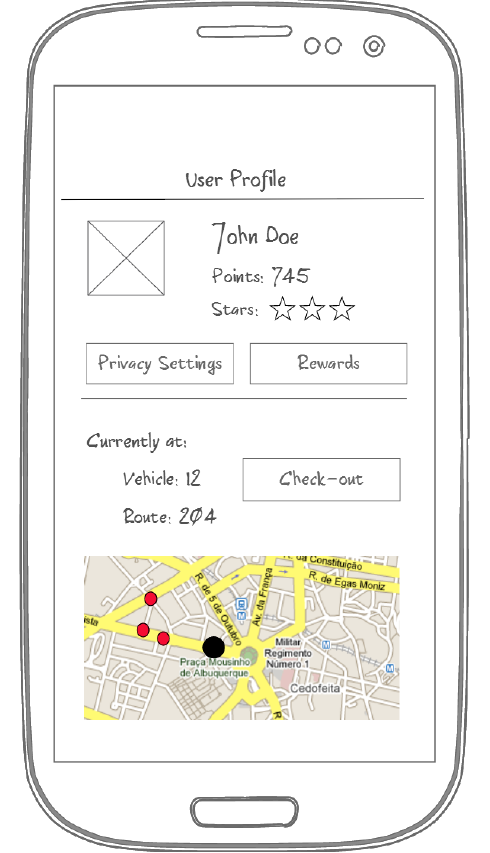
\includegraphics[scale=0.5]{profile1.png}
    \caption{Initial draft of the user profile screen - with network user map.}
    \label{fig:profile1}
  \end{center}
\end{figure}

\begin{figure}[h!]
  \begin{center}
    \leavevmode
    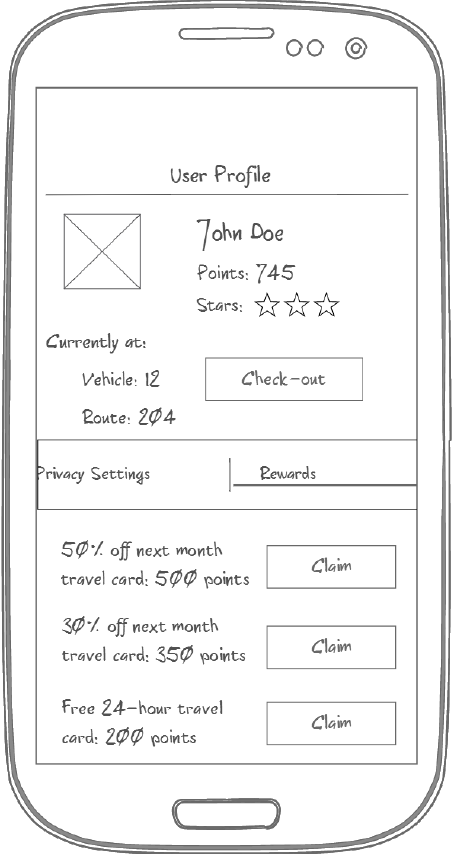
\includegraphics[scale=0.5]{profile2.png}
    \caption{Initial draft of the user profile screen - without network user map.}
    \label{fig:profile2}
  \end{center}
\end{figure}

For the first possibility (the one with the user map), it was also considered that a touch on a user on the map could display a dialog with a short profile of that user (username, points, stars and photo/avatar). That could, however, bring some usability difficulties due to the size of the elements that would represent a user on the map and would probably too small for this type of devices, where the touch gestures generally have low precision.

\subsection{Comment, Rate and News Feed}\label{rateinitial}

As said before, having the rate functionality separated from the news feed could have been the origin of the difficulty perceived by the users on grasping the feature. Explaining the feature in a more detailed way, after the submission of a comment by a user, that comment would be sent for two random people in the same network, who could verify the correctness of the information. 
The chosen users would then receive a notification informing them that there were comments left to rate. Only after successfully rated by two users, the comment would be published and available to other users in the network.

Two problems emerge from this system: first, there is the risk of an insufficient number of users in the network to perform the validation; second, because the comment would only be published after two successful ratings, there was also the risk that when those conditions were met the information would not be useful anymore.

The conceived solutions encompassed the aggregation of the rating feature with the news feed, with the 'must-rate' comments from other users appearing with a visual highlight (another background color, for example).
Both of those solutions involved as well showing the users' own comments in the news feed, aligned to the other side of the screen and also with a different background color to the message, resembling the behaviours usually seen in instant messaging or chat applications, that were since then applied to SMS applications on mobile devices.

The difference between the two solutions is that one of them includes the aggregation of the comment features in the news feed tab as well (joining the comment, rate and news feed features all-in-one) - Figure \ref{fig:comment2} - while the other maintains two distinct tabs, one for news feed and rating and another one for submitting a comment - Figure \ref{fig:comment1}. 
Both these solutions were also conceived with the realization of a focus group session in mind, in order to promote the discussion about these features and the interaction associated with them.

\clearpage

\begin{figure}[h!]
  \begin{center}
    \leavevmode
    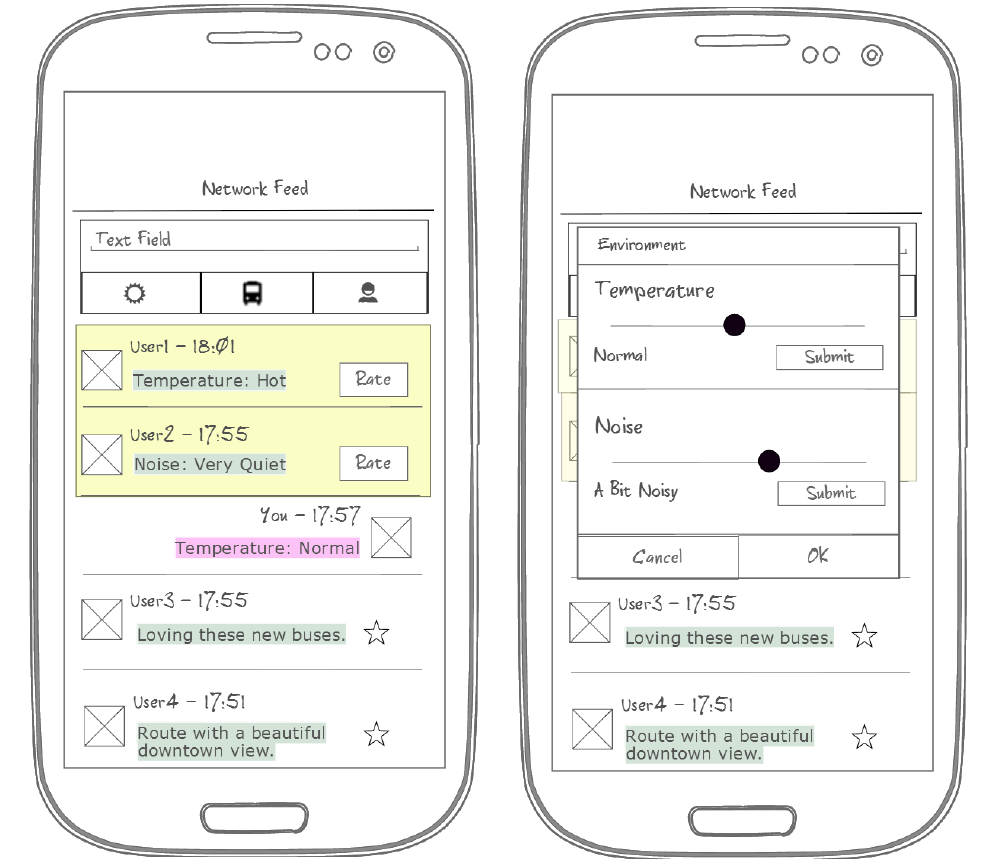
\includegraphics[scale=0.5]{comment2.png}
    \caption{Initial draft of the comment, rate and news feed features - all-in-one.}
    \label{fig:comment2}
  \end{center}
\end{figure}

\begin{figure}[h!]
  \begin{center}
    \leavevmode
    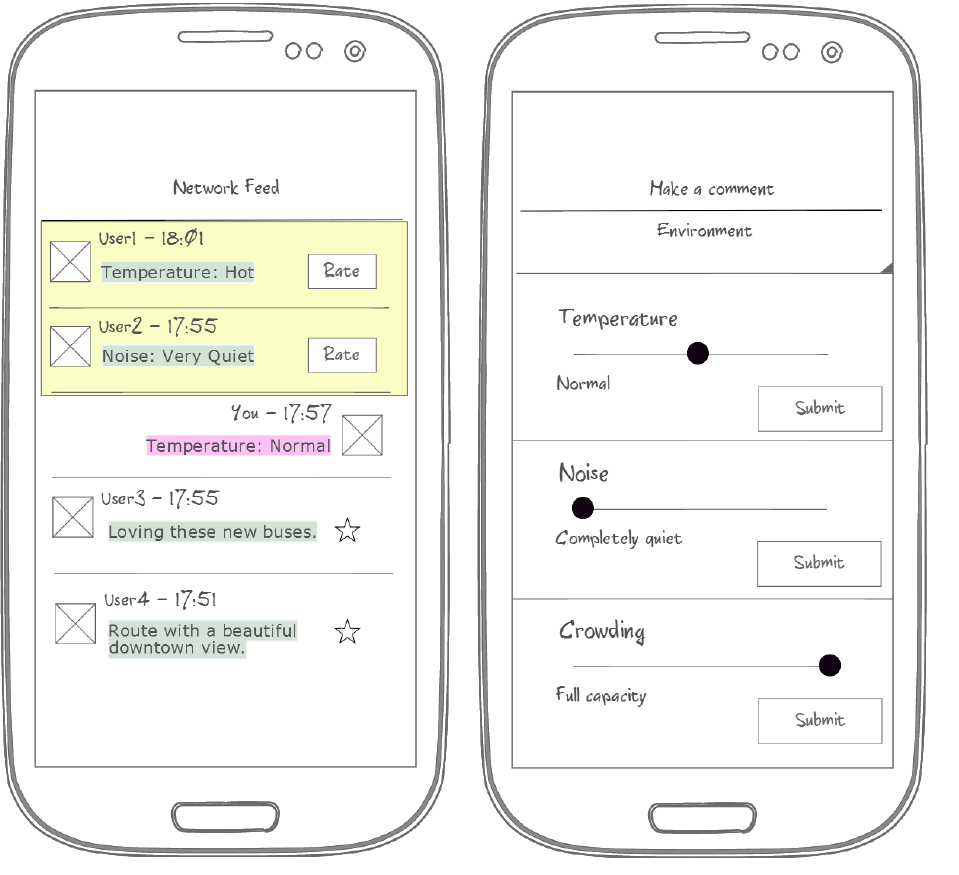
\includegraphics[scale=0.5]{comment1.png}
    \caption{Initial draft of the comment, rate and news feed features - news feed/rating aggregated, with comment in other tab.}
    \label{fig:comment1}
  \end{center}
\end{figure}

\subsection{Journey Planner}\label{jourplaninit}

The previous iteration of the project included a journey planner feature, that could be used by passengers to indicate trips they intend to make in the near future. Ten minutes before the chosen start time for the trip, the users would receive a notification reminding them of the planned trip and asking if they desire to receive information in real-time about the trip.

This feature has some importance in the application concept, because it may allow the system, in the future, to collect data related to the user trip profile, in order to predict, suggest and inform him about trips performed in a regular basis.

However, despite that possibility of planning a trip, after introducing that plan in the application, the user could not see the introduced plans. This was probably conceived this way to allow a user to plan just one trip for the next hour or so, but if a user wants to plan several trips for one day or week, there is no possibility of checking those trips, putting on the user all the effort to remind them.
Thus, a schedule feature was conceived, in order to give users that possibility, with the goal of catching their interest about the journey planner features.

The existing tab referring to the journey planner was maintained, adding one more screen to that tab (the schedule feature). That included the need for a secondary navigation that would allow the user to choose either the planner or the schedule tab. The considered solutions were a second set of tabs, or a spinner where the user could select the desired option (see Figure \ref{fig:planner1}). These solutions would also be presented at a focus group session (section \ref{focusgroup}) for discussion.

\begin{figure}[h!]
  \begin{center}
    \leavevmode
    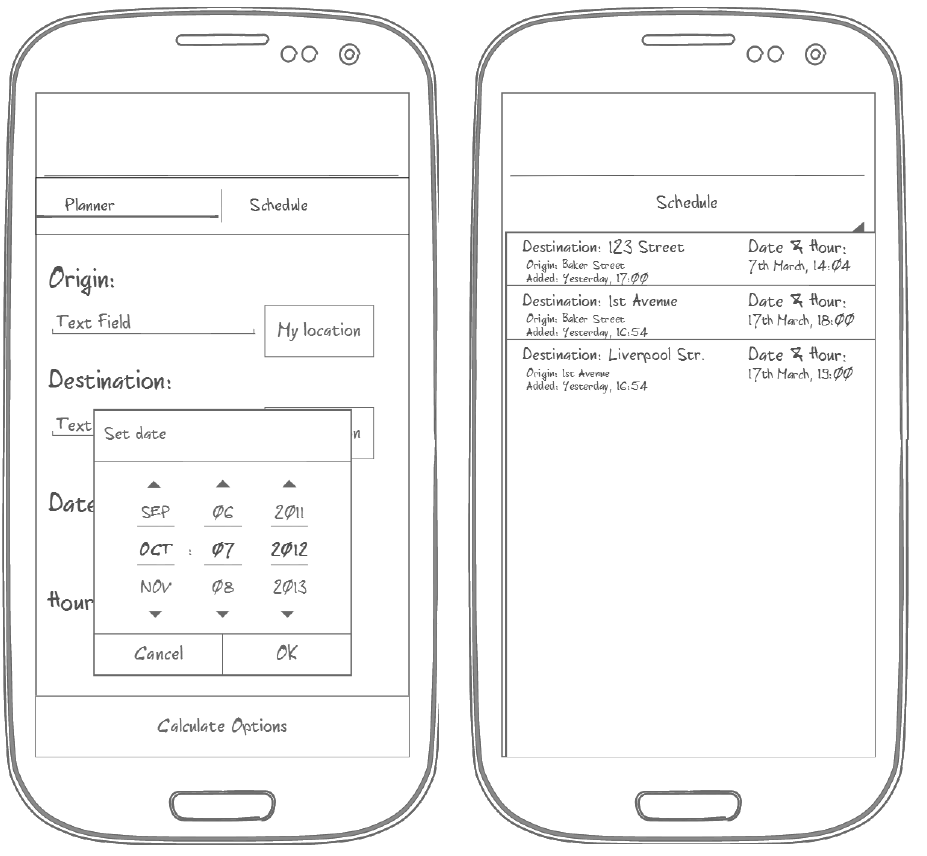
\includegraphics[scale=0.5]{planner1.png}
    \caption{Initial draft of the journey planner features - with tabs on the left, with spinners on the right.}
    \label{fig:planner1}
  \end{center}
\end{figure}

\section{Focus Group}\label{focusgroup}

During this phase, in order to define and specify usability requirements, a focus group session was held at \emph{IBM-CAS} room at FEUP.

Focus groups consist in an informal technique used to understand user needs and feelings \cite{kn:KC08}. This technique can be used at any stage of the development phase, before the design phase or even after the implementation, with the goal of discussing issues and concerns about the features of an user interface. 

These sessions usually bring together between six and nine users, typically lasting about two hours. A moderator should be assigned to the session, in order to maintain the group's focus \cite{kn:Nie97}. 

In this case, the main goal for the session held was to understand what users needed, presenting them the alternatives mentioned on the previous section to discussion. Note that these kind of sessions are not intended to evaluate interface usability (because usually participants do not have the chance to use the product on their own, but instead a demo is presented to the whole group). In this particular case, it was intended to check if the application could solve some of the users' problems regarding public transport information, what could be done to improve that matter and changes regarding the interaction that could lead to that improvement.

Six participants with different backgrounds, age groups and different patterns of public transport use were part of the session. In Table \ref{tab:table1}, is it possible to see those characteristics in more detail. \\ \\



\begin{table}[H]

\begin{center}
\begin{tabular}{ c c c c p{5cm} }

  \hline 
  \textbf{\#} & \textbf{Gender} & \textbf{Age Group} & \textbf{Public transport usage profile} & \textbf{Background} \\
  \hline 
  1 & Male & 18-25 & Frequent subway user & Public transport related Msc. thesis
   student \\
  \hline
  2 & Female & 18-25 & Occasional bus and subway user & HCI related Msc. thesis student \\
  \hline
  3 & Male & 40-60 & Occasional bus and subway user & 20+ years experience with public transport
  network studies (customer satisfaction
   and scheduling) \\ 
  \hline
  4 & Male & 18-25 & Frequent bus and subway user & Msc. Student in Services Engineering
   and Management\\
  \hline
  5 & Male & 25-40 & Occasional bus and subway user & PhD. Researcher in public transport
   networks field\\
  \hline
  6 & Female & 40-60 & Occasional bus and subway user & PhD. in Operations Research\\
  \hline
\end{tabular}
\caption{Focus group participants characteristics.}
\label{tab:table1}
\end{center}
\end{table}

As expected, a lot of ideas came up from the session. However, the ideas and discussions pointed in a way where a major redesign or rethinking about the application concept was needed.

For instance, assume that a user wanted to perform a journey between a given point, A, and another given point, B. To go from A to B, there are several options, transportation methods and routes. In the way the concepts behind the application were currently designed, there was no way that the user could use it in order to make a informed decision about his trip. 

If there are three possibilities to go from A to B, two being distinct bus routes and one being subway, it is useful to the user to check if there is some problem regarding one  or two of these routes (delay, traffic jam, accident and so on) and possibly change the option he would take, saving him time and trouble by giving him the information to perform that informed decision.

Even if the user desires to receive information about other journeys (if they do several different journeys between different points in one way or through the week), this was also impossible to get with the application.

In short, the following problems were faced: 

\begin{itemize}
\item Impossibility of checking the information before entering the vehicle - as the user had to check-in in a route and vehicle prior to  submit and, more importantly, to receive information. 
\item Impossibility of checking more than one route at a time - User only could receive information from the route where he was checked-in, and could only be checked-in at one route. 
\end{itemize}

If the possibility of receiving information for several trips was introduced, one of the suggestions was the possibility to filter which trip (or trips) the user wanted to see information from, in order to not get lost in the middle of a big volume of information. Taking the same example situation above (three possible routes between A and B), a user should be capable to, despite receiving information from the three routes, to hide one or other just to make the visualization of the information easier, showing it again whenever he wants to. 

The discussed solutions referring user profile information (Figures \ref{fig:profile1} and \ref{fig:profile2}) resulted in the conclusion that the users do not feel comfortable seeing the other users in their temporary network, because that would imply their information would be accessible to other users as well. 

Instead, they valued the existence of a record with the user journeys and user statistics about some of the aspects of their journey profile.

All users recognised value in the existence of the schedule feature (Figure \ref{fig:planner1}), and suggested as well the existence of favourite trips, which could easily be added to the trips the user desires to receive information from.

About the interactions proposed, the main navigation composed by tabs with icons and labels (Figure \ref{fig:tabs2} and \ref{fig:tabs3}) was considered a good way to go. The feedback about the secondary navigation was mixed, but the secondary set of tabs (for journey planner) was considered easier to learn, because the user does not have to open the spinner widget to see all the available options in the secondary navigation.

Some others conclusions pointed to the importance of the rewards given to the users, to improve user engagement with the application, and that the trip aspects that the users value the most are related with security and service quality.


In the following chapter it is possible to see the changes that the gathered data and conclusions introduced to the application concept and its features and interaction.

\chapter{Application Development} \label{chap:chap5}

\section*{}

This chapter covers in detail the development phase for the application, starting with the suggestions obtained in the performed focus group to evolve the initial drafts all along to the implementation phase. In the section \ref{interfacecon}, that process will be described, concept by concept.

\section{Architecture}

\subsection{Data Model}

The data model for this application was initially the same conceived and referred in \cite{kn:Gonc12}. That said, it carries the same assumptions and limitations then assumed, such as the simplified network concept (where a network is not centred in the user, as desired for the future, but represents a single line and direction).
Therefore, checking-in in a network represents sharing information with other users in the same line or direction, where it should represent sharing information with users performing trips in a set of routes, lines or directions with relevance to the pair origin-destination where the user checked-in.

The same data model was refined in a second iteration of the project, aiming to give additional intelligence to the application, by calculating relevant routes for a given origin and destination. The relevant routes are calculated through inferring from past data from validations supplied by \emph{STCP}, and users in routes considered relevant are due to be added to the initial user temporary network (the same who provided the origin and destination used to perform that calculation) \cite{kn:Dia13}.

The refined data model introduced another change: the usage of transport public data from the city of Porto, while the older one used data from \emph{Transports from London}(TFL), which were used in the tests performed in the field among users. 

In this work, some adaptations to this recent version of the data model were made, in order to allow some concept modifications. Those adaptations will be mentioned and explained in the following sections, along with the reasons that lead to them.

\subsection{Android Application}

As said before, the technology chosen for the functional prototype of the application is \emph{Android}. This choice was made due to several reasons. 

The first reason is portability. \emph{Android} applications are developed in \emph{Java} (although, a modified version of \emph{Java}, along with \emph{XML}). \emph{Java} code is compiled to run in any Java virtual machine, making it possible to develop applications in any environment, either it is \emph{Windows}, \emph{Linux} or \emph{Mac OS}.

The choice about target version has fallen on the \emph{Ice Cream Sandwich} API, which, as mentioned in section \ref{technology}, has several advantages regarding UI design and implementation and interaction patterns. 

This choice was reinforced by an additional point: Android Cloud to Device Messaging Framework, that allowed push notifications to be sent to the application. Those notifications would allow the rating feature as it was conceived previously, prompting 2 random users from a network to rate a submitted comment from that network. However, Cloud to Device Messaging Framework (C2DM) has been deprecated in July 2012, being replaced by a new service, Google Cloud Messaging (GCM).

If the maintenance and refactoring of the code that made that rating feature work in the previous application (and webservice) was a point in favour of adopting \emph{Android} 2.2 for the implementation of the application, that change (allied to the already pointed limitations of the existing rating system), were strong points against it.

\subsection{Webservice}

The webservice connecting the existing database (as well as other data concerning the route relevance calculation) and the mobile application was also the same developed in \cite{kn:Gon12}.

Similar to what was said about the data model, it was made an effort to integrate, when possible, the existing webservice with the new application prototype. However, some concept and feature changes required changes to the webservice as well. Those changes will also be mentioned in the following sections, when explaining what lead to them.

\clearpage

\section{Interface Elements and Concepts}\label{interfacecon}

This section will cover the evolution of the interface and interaction of the application during the design phase, as well as a detailed explanation about how the implementation of the designed interface was made.
All the design guidelines and examples that were in the origin of design choices are also explained. However, it must be said that usability guidelines rarely consist in hard and fast rules, and usability questions frequently don't have just a single answer. In most cases, there are design trade-offs that must be considered \cite{kn:MobileUsab}.

\subsection{Branding}

Despite being an application directed to the public, or intended to be in a near future, the attribution of a name or image associated to it was missing or yet to be discussed.


In a discussion with Eng. António Nunes, the creator of the idea behind the project, some thoughts and suggestions about a possible name for the application came up. For this iteration of the project, one of them (proposed by him) was selected - Journata.

This name was selected because in the opinion of the people involved in the project, it could give the user an initial perception about some of the application features - it can be considered a travel journal in some way - while performing a word play with the words "journey", "journal" and "data". Even the name itself, Journata, resembles the Italian and Portuguese words for "journey" - \emph{giornata} and \emph{jornada}, respectively.

Some thought was also put in creating a logo for the application. The main idea was to resemble a public transport vehicle (bus or subway), while giving a modern look to the referred vehicle and to the logo itself. In the following figure, it is possible to find the designed alternatives for a first logo of the application. 

\begin{figure}[htb]
  \begin{center}
    \leavevmode
    
\includegraphics[scale=0.2]{logo_versions.png}
    \caption{Application first logo alternative designs.}
    \label{fig:logo}
  \end{center}
\end{figure}

The middle option was then selected to be part of the prototype.


\subsection{Main Navigation}

After the realization of a focus group session (see section \ref{focusgroup}), the design choice had fallen over a tab navigation, consisting in four tabs, always visible.

Those tabs were meant to represent:

\begin{itemize}
\item News Feed
\item Comment Submission
\item User Profile
\item Journey Planner
\end{itemize}

The design decision about the existence of text labels as an additional information (along with suggestive icons) was made in order to make the learnability of the interface easier. There are several well-known mobile applications who use tabs as their main navigation component, and social networks are no exception. In the following figure, it is possible to see a screenshot of the \emph{Facebook} application for \emph{Android}. 

\begin{figure}[htb]
  \begin{center}
    \leavevmode
    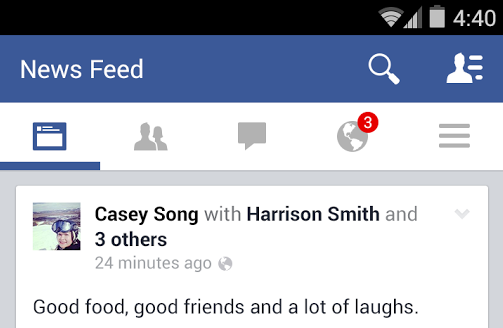
\includegraphics[scale=0.6]{facebook1.png}
    \caption{Screenshot of \emph{Facebook} application navigation component for \emph{Android}.}
    \label{fig:facebook1}
  \end{center}
\end{figure}

Here, it is possible to see that the chosen navigation does not have text labels with additional information about the features they refer (in some cases, textual information about the feature can be seen in the Action Bar, though). However, in this case it is considered acceptable, since \emph{Facebook} users know the displayed icons very well and associate actions and meaning to them, since the same icons are displayed in the \emph{Facebook} website for years and users know pretty well what the actions associated to them (preserved in the mobile application).


A distinct example can be \emph{Swarm}. This recent application, from the creators of \emph{Foursquare}, has a tab-based navigation as well, but because users are not yet familiar with the features associated to those icons, there is an initial difficulty in the application learning process.

\clearpage

\begin{figure}[htb]
  \begin{center}
    \leavevmode
    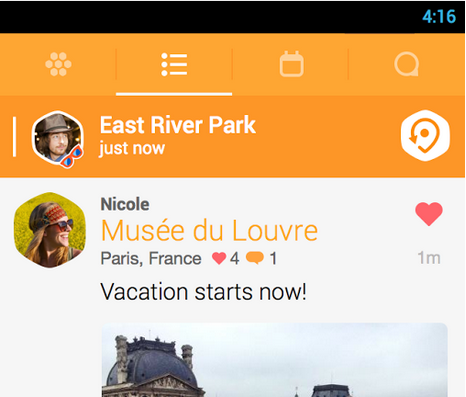
\includegraphics[scale=0.6]{swarm1.png}
    \caption{Screenshot of \emph{Swarm} application navigation component for \emph{Android}.}
    \label{fig:swarm1}
  \end{center}
\end{figure}



Other reason to provide textual information labels along the icons is the widespread usage of those labels in \emph{iOS} applications, where tab navigation is fairly common, despite being in the bottom of the screen.

\begin{figure}[h!]
  \begin{center}
    \leavevmode
    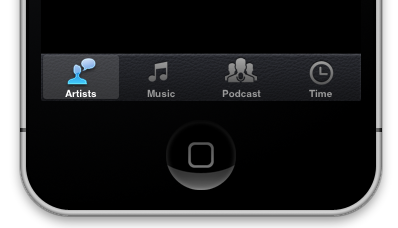
\includegraphics[scale=0.6]{ios_tabs.png}
    \caption{Example of a tab navigation in an \emph{iOS} mobile application.}
    \label{fig:ios-tabs}
  \end{center}
\end{figure}


\subsubsection{Iterations}

One of the first decisions after the focus group was to re-order those tabs by perceived importance. The information in user profile was perceived as less important than the journey planner features (or at least it is intended that the journey planner features have more visibility). To accomplish that, the journey planner tab was then moved to third place (from left to right), switching its place with the user profile tab.

The label associated to the journey planner tab was also changed in order to inform the user that that tab included some more features but not just the planner, such as a list of favourite and scheduled trips.
It is possible to see the result of that decision in figure \ref{fig:mainnav3}.


\begin{figure}[h!]
  \begin{center}
    \leavevmode
    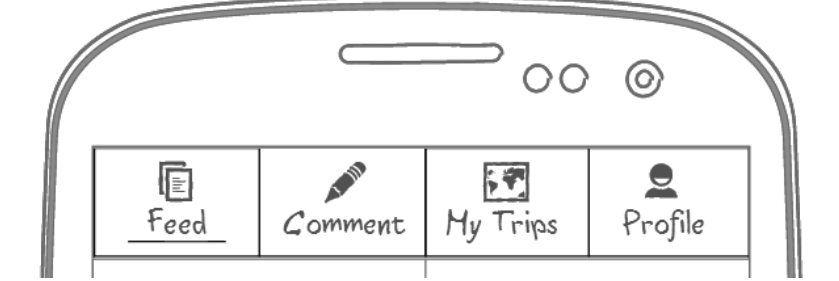
\includegraphics[scale=0.6]{mainnav3.png}
    \caption{Second iteration of the tab navigation interface.}
    \label{fig:mainnav3}
  \end{center}
\end{figure}

This new version of the interface was not changed until the end of the design phase, when it was the subject of an usability test along with the remaining components of the interface(see Appendix \ref{ap2:usabtest}) and consequently validated.

\subsubsection{Implementation}

In the implementation of this component, an external library (ViewPagerIndicator \footnote{\url{http://viewpagerindicator.com/}}) was used and customized in order to facilitate the integration of swipe gestures to alternate between tabs. This way, a more fluid interaction was made available to the user.

The \emph{Android} Action Bar was also used, despite not being part of any of the interface design, to include elements such as the application name, logo and an option menu with features missing in the design iterations.

\begin{figure}[h!]
  \begin{center}
    \leavevmode
    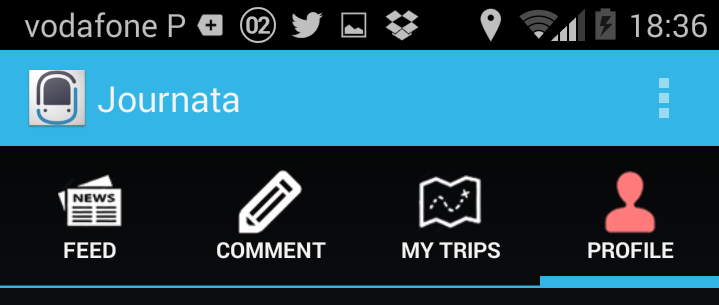
\includegraphics[scale=0.8]{mainnav4.png}
    \caption{Screenshot of the implemented application's main navigation.}
    \label{fig:mainnav4}
  \end{center}
\end{figure}

\subsection{News Feed}\label{newsfeed}

After the performed focus group, one of the suggestions consisted in the introduction of feed subscriptions. The user could receive information from several networks (instead of just one, as previously established), subscribing an information feed of each network for that matter. 

\subsubsection{First Iteration}

An initial thought on that suggestion resulted in considering the possibility of having several check-ins at the same time. The first design iteration after the realization of the focus group was aligned with this idea. Subscribing a network feed (the act of adding the subscription) therefore implied the check-in of the user in the same network. 

Four new features were then considered: 

\begin{itemize}
\item Add a new feed subscription (previously there was no need to add, since the network were the user was checked-in was the one whose information was displayed);
\item Listing the current feed subscriptions;
\item Removing a feed subscription;
\item Filter visible feed subscriptions (the 'view feed' feature would display a 'global feed', with all the feeds subscribed. With this filtering, the user could mark one or more feeds to be invisible in the 'global feed').
\end{itemize}

The need for the existence of a secondary navigation (similar to what was discussed for journey planner features in section \ref{jourplaninit}) presented itself in this component as well. For better coherence between secondary navigations in other tabs and for improved visibility of all the available options to the user, a secondary set of tabs was chosen.

To subscribe a new feed, the user would indicate the origin and the destination of the network from which he desired to retrieve information (the origin or destination could be based on the user's GPS location, searching the nearest stops), as well as the date and hour for the information. 
Then, the user would retrieve a list with several options, listing all the vehicles and methods of transportation available at the supplied date and hour. To make the list item selection easier, a button to select/deselect all the options would be available as well.

That way, if an user wanted to retrieve information between A and B, and three possible transportation methods/vehicles are available, the user would need to select all the three of them in order to get information from all those lines and perform an informed decision (see figure \ref{fig:feed_iter1_add}).

\begin{figure}[htb]
  \begin{center}
    \leavevmode
    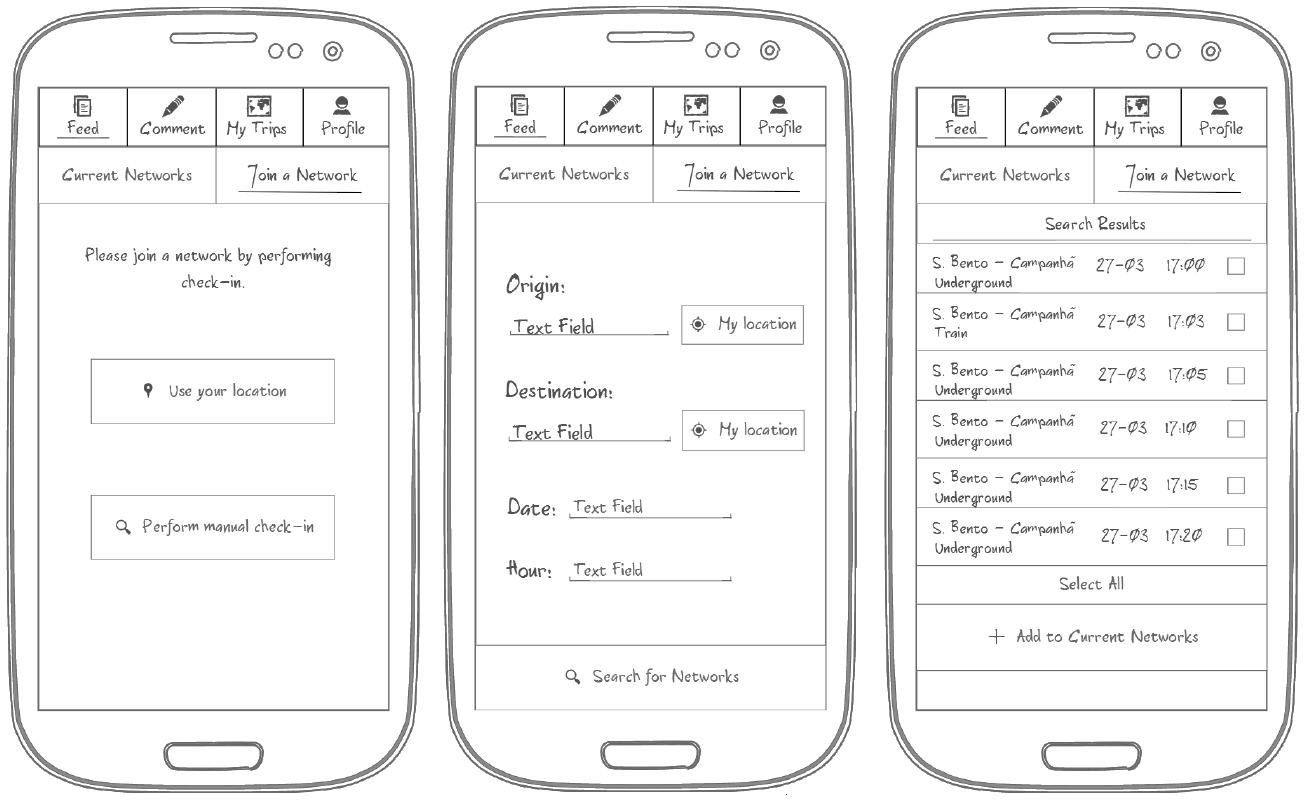
\includegraphics[scale=0.4]{feed_iter1_add.png}
    \caption{News Feed features and screens - Add Feed, First Iteration.}
    \label{fig:feed_iter1_add}
  \end{center}
\end{figure}


However, this design had several limitations. For example, the user usually has a hard time identifying the exact vehicle he's in (despite the fact that an hour on the schedule can be used to identify the vehicle, that vehicle can be running late, for instance. In case of transportation methods that have high frequency, such as subway, the difficulty of such a task is even higher).


This would also bring an additional problem - along with adding a feed subscription for every transportation method for the chosen course, the same was required for removing those feeds.
By clicking on an item of the list, representing a feed, a menu would also be available to the user, allowing him to remove a feed. When an item was selected to removal, a confirm dialog would be presented to the user. However, this is considered as something to avoid when designing mobile applications because of the additional effort presented to the user (additional interaction).

The 'filter visible feeds' feature was designed as a list where the users could mark each one of the current subscribed feeds as visible or invisible, through a check-box. However, it was considered that the use of a check-box to perform this selection was not efficient, because it was not clear enough to the user what were the practical effects of that selection and the actions triggered by it (figure \ref{fig:feed_iter1_filter}).

\begin{figure}[htb]
  \begin{center}
    \leavevmode
    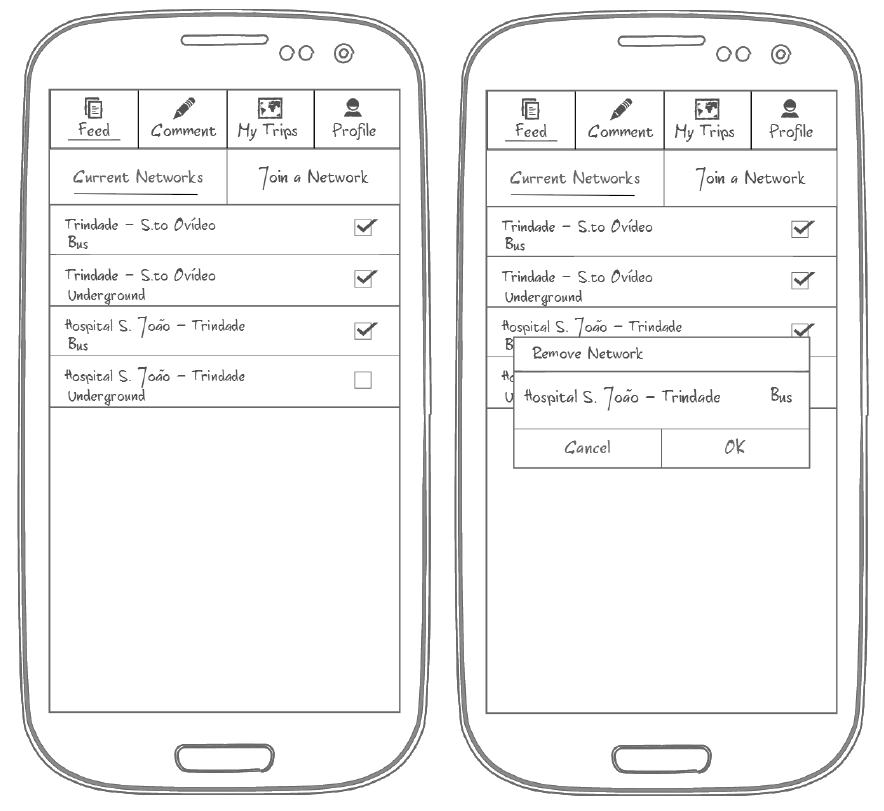
\includegraphics[scale=0.5]{feed_iter1_filter.png}
    \caption{News Feed features and screens - Filter and Remove Feeds, First Iteration.}
    \label{fig:feed_iter1_filter}
  \end{center}
\end{figure}


Viewing the news feed was considered the main and most critical feature of the application. Therefore, the need for a major redesign of this feature was recognized, because in the previous developed prototype, this feature, despite providing the functionality to the user, was not sufficiently attractive or displayed enough information to the user.

The first thoughts about this feature included what should be the information displayed to the user in each comment from a feed.
Since this was no longer a feature associated to a single route or network, every item should have the indication of the network it refers to, consisting in origin, destination, transportation method and route number (this one is only valid if it refers to a bus route).

In order to make this feature more attractive, and since between the fields available in a user profile, a photo was also considered in the initial work \cite{kn:Gon12}, an interface similar to the message display we encounter in several instant messaging or SMS sending applications for mobile devices (such as \emph{Google Hangouts}, \emph{Android} SMS application), where the user or contact photo is displayed near the content of his message.

In this case, and opposed to what was previously done, the appearance of the user's own messages along with messages from other users was conceived, in order to create that effect and to give the user a sense of contribution to the community of the users of the application, trying to improve their levels of engagement.

A different highlight color for the user's own comments was also selected, in order to differentiate them from other users' comments, and it was also conceived that those two types of comments should be aligned each one to a different side of the screen.

Each item would also have the option to give a star to the comment author, if the comment in question was considered particularly helpful. 


As said before, it was decided to aggregate the comment feature in the view feed screen, and the initial thought in how to do that was to highlight the items with pending user review in the top on the feed, despite possibly being older than some of the already approved comments. Those comments would also have a button that, when triggered, would prompt a dialog to the user making it possible to define and submit the rating about the referred comment (figure \ref{fig:feed_iter1_view}).

\begin{figure}[htb]
  \begin{center}
    \leavevmode
    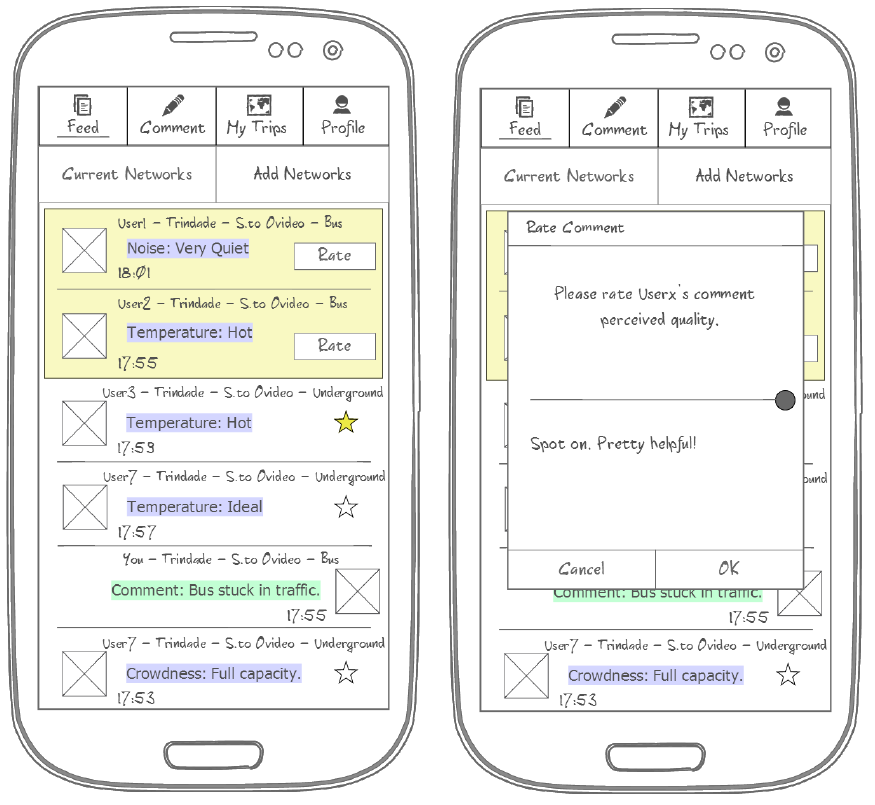
\includegraphics[scale=0.5]{feed_iter1_view.png}
    \caption{News Feed features and screens - View Feed, First Iteration.}
    \label{fig:feed_iter1_view}
  \end{center}
\end{figure}




\subsubsection{Second Iteration}

Recognising the existing limitations in the first design iteration,  a second iteration was made, based in the assumption that subscribing a network feed would be independent from check-in. This way, the existence of a check-in was not required to receive information. The need for defining date and hour when adding a new feed subscription was also eliminated.

However, the most relevant change for this new iteration was the aggregation of the feeds for several transportation methods in just one. According to this new paradigm, if the user wants to receive information between a given point A and another given point B, he would only need to subscribe one feed, defining the origin as A and the destination as B. The subscribed feed would then include all the information of all the possible routes to go from A to B, as well as other relevant routes (integrating this concept with the work developed in \cite{kn:Dia13}), independently from the transportation method. 

This way, for the previously given example, where the user has three distinct routes or options to go from A to B, the same user would subscribe an unique feed that would allow him to retrieve information from all of the three options.

The screen for adding a new feed subscription was also redesigned, having now an additional button allowing to switch the content of the text fields of origin and destination (an interaction pattern encountered on other mobile applications that present the input of similar data to the user, such as \emph{Google Maps} or \emph{Moovit}).
Several alternatives for that screen, intended to highlight and at the same time facilitate the option for choosing the current location of the user as origin or destination, were also designed (figure \ref{fig:feed_iter2_add}).

\begin{figure}[!h]
  \begin{center}
    \leavevmode
    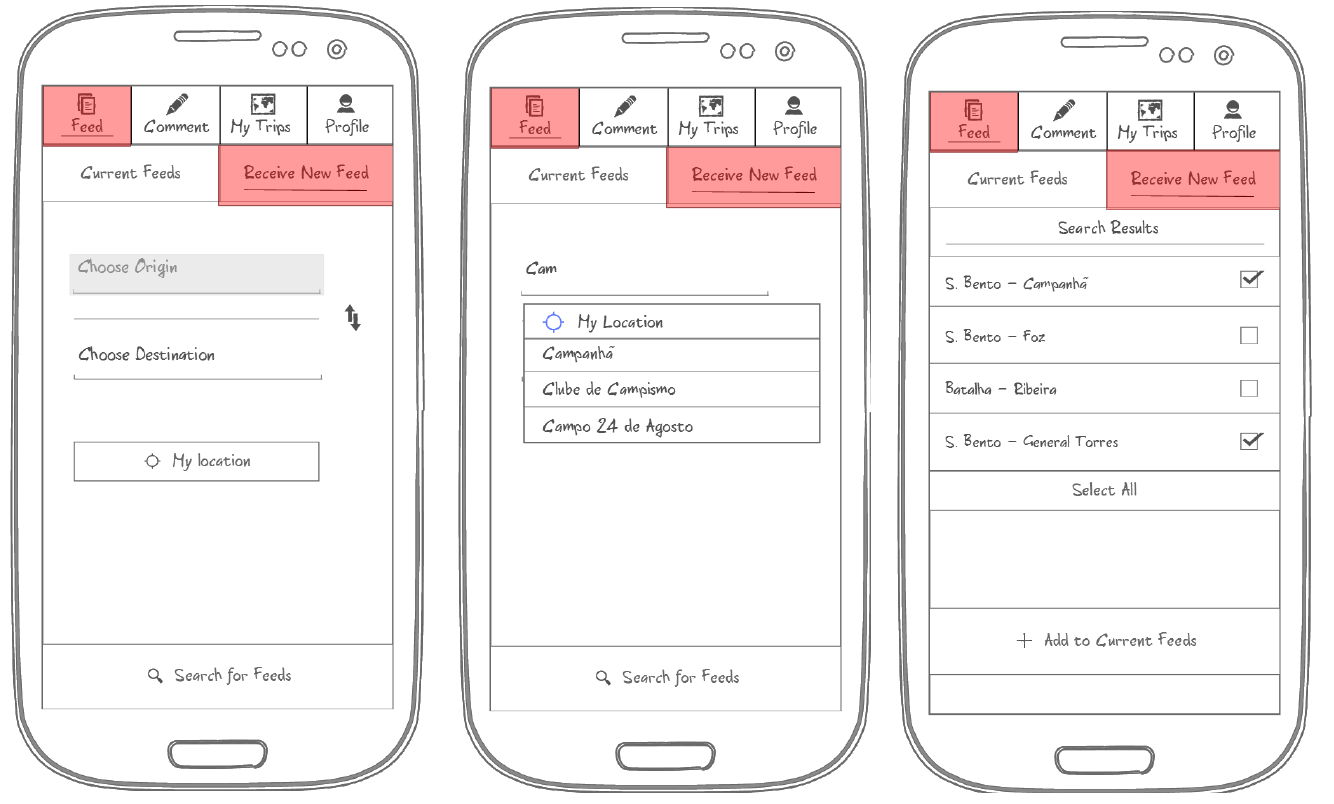
\includegraphics[scale=0.5]{feed_iter2_add.png}
    \caption{News Feed features and screens - Add Feed (alternative designs) and Search Results, Second Iteration .}
    \label{fig:feed_iter2_add}
  \end{center}
\end{figure}


Regarding the filter feeds feature, the check-box from the first iteration was replace by a switch with textual information about the feed status/action associated to it.
To the menu where it was possible to find the option to remove the feed from the list of subscribed feeds, the option to add the same feed to the list of favourites (see section \ref{journeyplanner}) was also added. 

The confirmation dialog for feed removal (or for any task at all) is considered as something to avoid when designing mobile applications. An interaction pattern that allowed to replace that sort of dialogs consists in removing the item, giving the user the option to undo the item removal for a few seconds. This pattern can be encountered in some \emph{Android} applications widely used, such as \emph{Gmail}. This interaction pattern was also considered for this feature, as it is possible to see in figure \ref{fig:feed_iter2_remove}.

\begin{figure}[htb]
  \begin{center}
    \leavevmode
    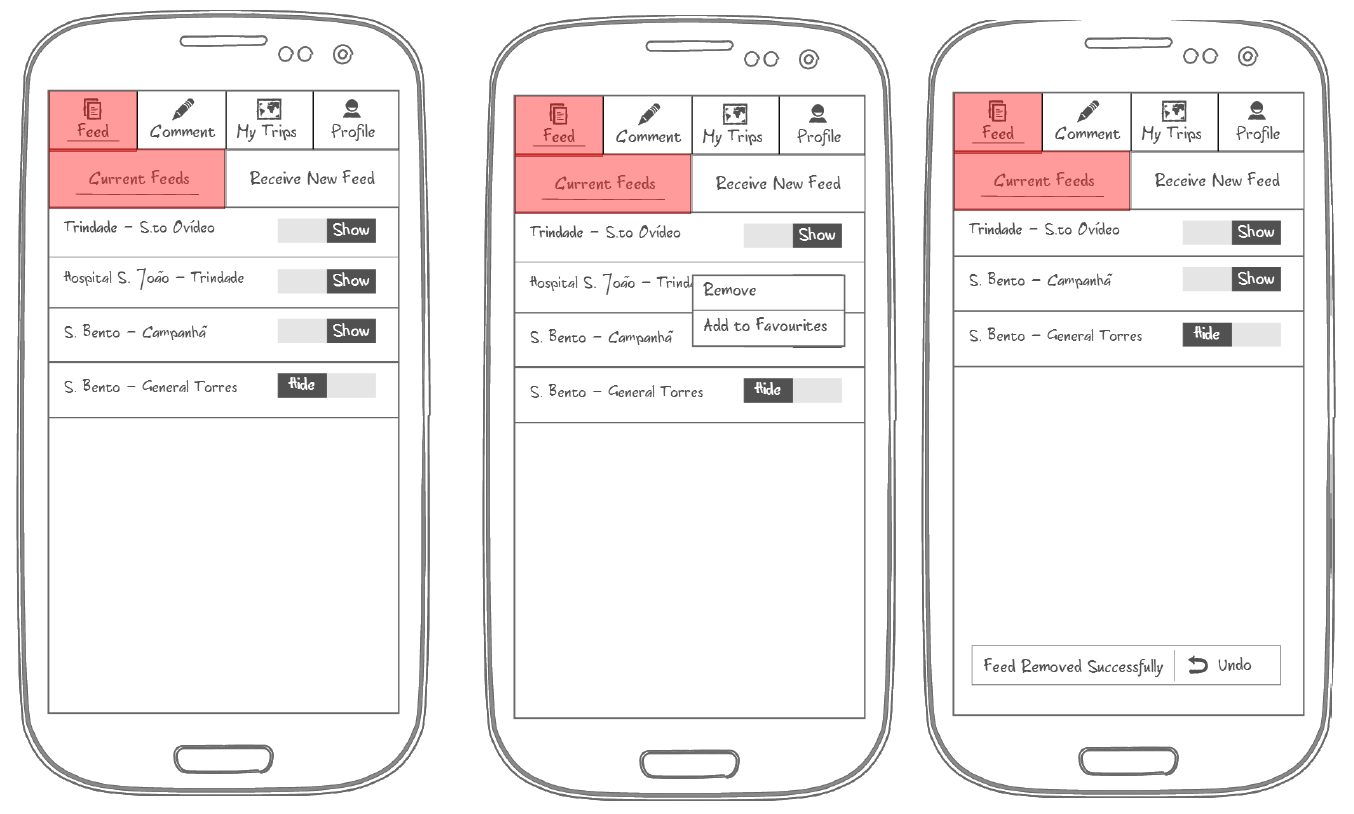
\includegraphics[scale=0.5]{feed_iter2_remove.png}
    \caption{News Feed features and screens - Filter and Remove Feed, Second Iteration.}
    \label{fig:feed_iter2_remove}
  \end{center}
\end{figure}

\subsubsection{Implementation} 

The implementation of this module of the application tried to follow as much as possible the design from the second iteration. Several screens for situations where no information was available were designed and implemented (for when the user does not have any feeds subscribed, prompting him to do so in order to benefit from the usage of the application. This was done following the principles for feedback referred on Dan Saffer's \emph{Microinteractions}\cite{kn:Saffer}).

One question that was not considered in the design phase was the transition between the 'View Feed' feature and the other features in this component, that had navigation between them through the utilization of a secondary navigation. For that matter, a new tab was added to that secondary navigation, in order to allow that transition and make it as easy as possible to the user (through the touch on the desired feature tab/button).

\begin{figure}[!h]
  \begin{center}
    \leavevmode
    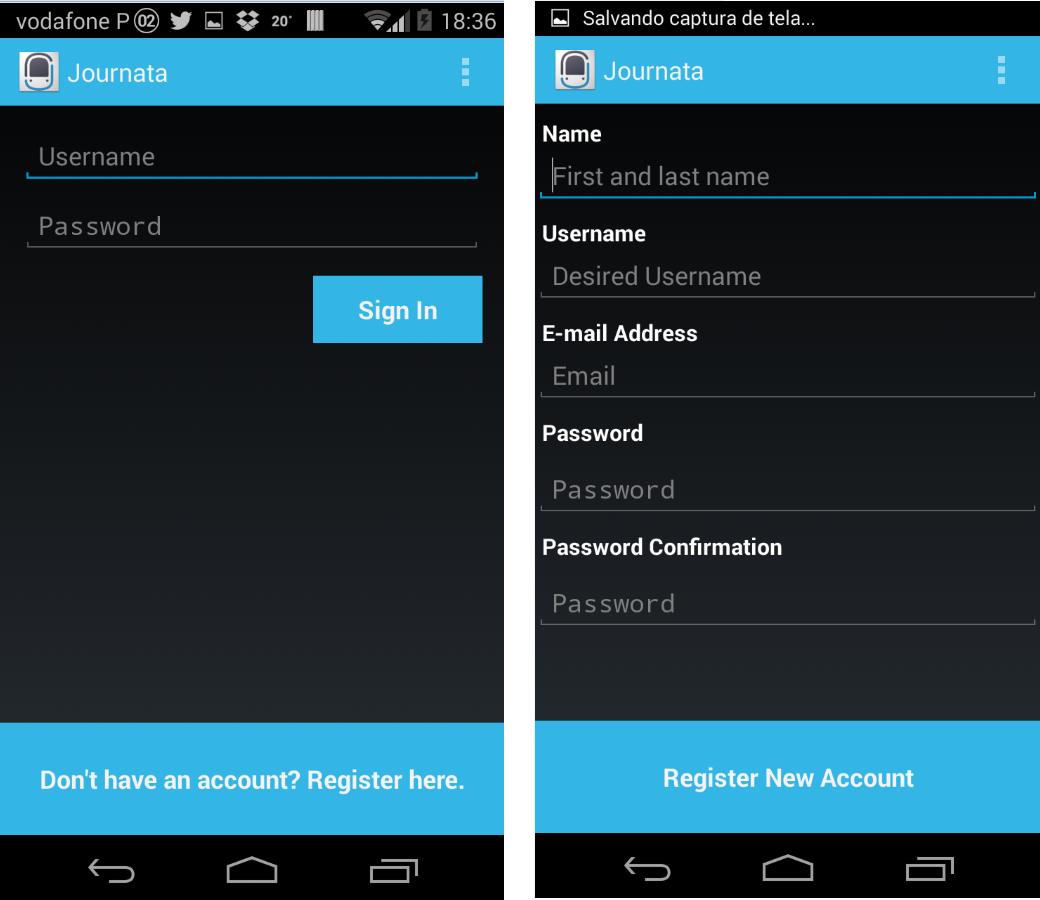
\includegraphics[scale=0.5]{login_register.png}
    \caption{Screenshots of the add and filter feed features.}
    \label{fig:feed1}
  \end{center}
\end{figure}

The form for adding a new feed used an improved version of the auto-complete used in \cite{kn:Gon12}. That was implemented in order to reduce the effort of text input from the user (it allows the user to select the desired bus stop right away). This form also allows the search to be performed without indicating one of the fields (origin or destination), providing all the possible options, something that was not possible in the previous application and that required changes to the existing API.

The list of retrieved results allows the selection of more than one result at a time, and therefore, saving the user from the effort of adding one feed at a time.
While waiting for the results, a progress bar is shown to the user, in order to avoid showing an empty list and inform the user that some action is occurring in the background.

A feature that was not included in the previous design iterations was the possibility of refreshing the news feed. This feature is available scrolling (pulling) the list of comments to the bottom of the screen. This feature was implemented with the use of the external library \emph{Simple-Pull-To-Refresh}\footnote{\url{https://github.com/JoeDailey/Android-Simple-Pull-to-Refresh}}. The implementation of this interaction pattern has become pretty common in applications where the user usually needs to fetch new information being displayed to him, such as an e-mail inbox, a news feed and so on. For instance, a similar implementation is part of the \emph{Gmail} application for \emph{Android}, as well as many social applications such as \emph{Facebook} and \emph{Foursquare}. 

\begin{figure}[!h]
  \begin{center}
    \leavevmode
    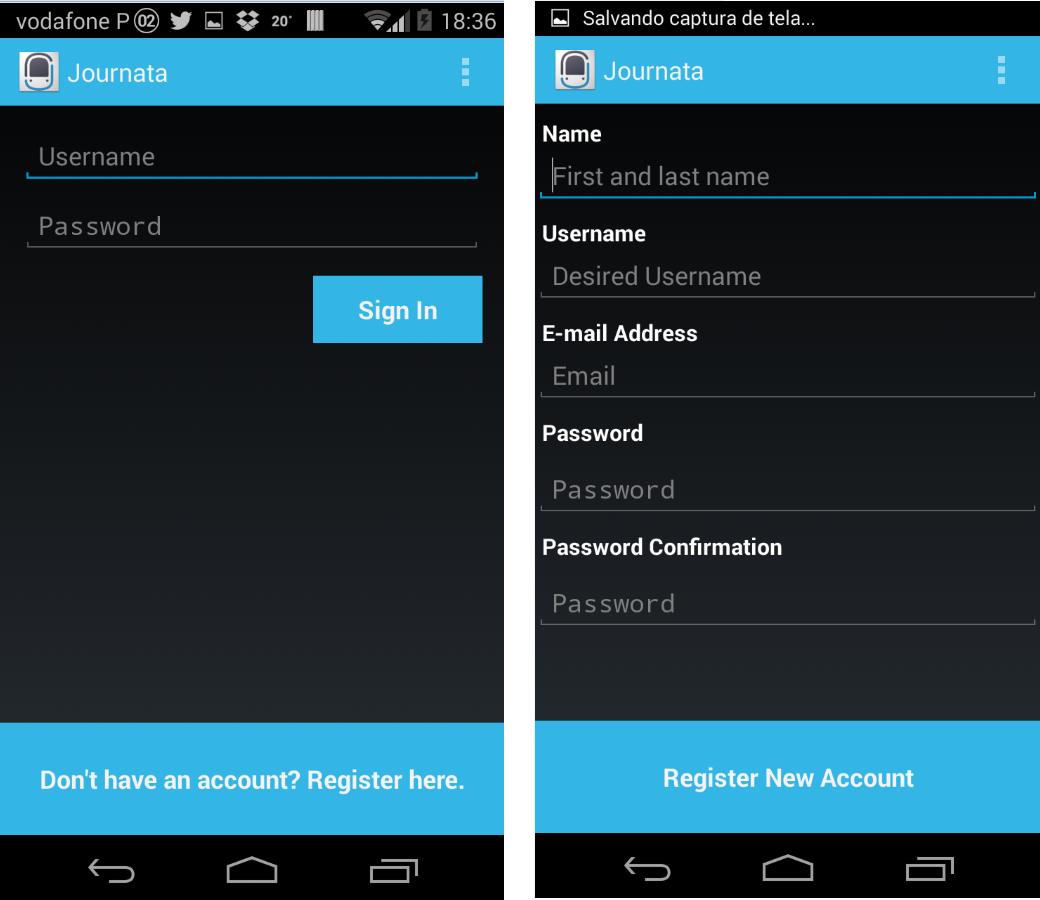
\includegraphics[scale=0.5]{login_register.png}
    \caption{Screenshots of the view feed feature (with refresh).}
    \label{fig:feed2}
  \end{center}
\end{figure}


Note that each comment has two buttons next to it, instead of the star that was part of the interfaces designed in previous iterations, and also that there are no highlighted comments prompting the user to rate them. This has been adapted due to changes in the point and rating system.

\subsubsection{Point System Redesign}\label{points}

The limitations identified in section \ref{rateinitial}, alongside with the deprecation of \emph{Google Cloud to Device Messaging Framework}, that was beneath the previous existing rating system, led to the development of a whole new (and simpler) rating system, consisting in giving a 'thumbs up' or 'thumbs down' to a comment. Each 'thumbs up' adds one point to the score of the comment in question, while a 'thumbs down' subtracts one point from that score. That comment score is called 'feedback', and comments with negative feedback score are hidden from the news feed of other users. 

This also lead to a creation of a new field in the data structure referring to the user data: feedback points, which is the sum of the feedback score of all of the user's comments. Due to the creation of the feedback points, it was also decided to eliminate the 'stars' that could be given to a very useful comment.

Those two buttons that can be encountered to the right of the displayed comments in figure \ref{fig:feed2}, with the shape of an arrow, represent the 'thumbs up' and 'thumbs down' actions.

In order to display the network feed information, additional changes to the API were made. The existing implementation required an existing login and check-in in order to retrieve the set of information from a network, retrieving only the information for the network where the user was checked-in. Changes to that 'request' method had to be made in order to retrieve data from any network without those limitations.

However, a problem that was not possible to overcome in a timely manner was that the existing data structure for representing the networks did not allow to fetch the origin and destination of those networks in the feed, despite what has been discussed in the design phase. The only useful information that can help the user identifying the network the information refers to is the number of the bus route (the current data set used only bus stops and routes from the city of Porto). This is expected to be corrected in a near future.

\subsection{Authentication}\label{authentication}

Authentication is obviously present in the majority of applications, because most of them have features that require a creation of a user account.

All the effort of doing that, however, has been reduced in many applications, through allowing registration via an existing account for a known and widely used social network or type of account. For instance, it is fairly common to encounter an application where registering an account can be made using our \emph{Facebook}, \emph{Twitter} or \emph{Google} account. In theory, the implementation of authentication via \emph{Google} account will require less effort, within the mentioned options, because \emph{Android} users have a \emph{Google} account associated to their mobile device and are usually already authenticated in that account when using it.

The main concern about reducing the registration effort to the user is related with the possible risk of abandon. Having extensive registration forms reduced the user motivation to continue that process and create an account (and consequently, to use the application). That concern is even bigger in mobile applications, where text input is harder and prone to user errors (small-sized keys, allied in most cases to writing while performing other tasks, such as walking).

That said, minimizing the text input is the way to go when developing mobile applications. However, that is not enough.

One of the most important guidelines for the development of mobile applications is to avoid making users pass through a registration screen as a starting point to use the application. 
When a user starts using an application for the first time, he has a low level of commitment. Unless the application offers immense value to him, as quickly as possible, users won't use it enough to make registration worth their while. 

Forcing users to register before they are sufficiently convinced of the value provided by the application will probably cause many of them to simply back out from it and never try it again, therefore losing the chance of causing a first impression \cite{kn: MobileUsab}.

This guideline is not exactly new, as it is recommended since 1999 in e-commerce sites (a user should be able to buy items without having to register). Its importance, though, is greater in mobile applications, because every extra step that the user must pass through causes considerable effort, and users are less committed to an app they just downloaded than to a website where they have spent time browsing before being prompted to create an account.

\begin{quote}
"Registration on the first screen is an example of 'take before you give': Apps want users to spend time and effort without any perceived benefit. Asking for permission to send notifications of use the current location before users find out what the app is about is another way in which apps abuse their emerging relationship with the users. Often users have no idea of the purpose of those actions (...).' \cite{kn: MobileUsab}
\end{quote}


In the scope of this application, it was decided that the elimination of registration as a first step was one of the tasks with greater level of importance. That prompted another decision - what would be the features accessible to non-registered or non-authenticated users in order to give them some value before creating an account. 

The chosen features, given that the decoupling of the check-in requirement in order to receive network information was performed (as referred in section \ref{newsfeed}), were the ones related with the news feed component. That included adding new feeds, filter the information about the received feeds and to see the news feed information. 
Those features represent, for users that don't want to contribute with comments to the platform, a way to still receive the information they desire, possibly motivating them to contribute in the future if they wish to do it.

For the remaining features, those that require being logged in, a screen informing them to do so, along with a visible button that redirects them to the login screen, appears if they are not logged in yet. 

\begin{figure}[h!]
  \begin{center}
    \leavevmode
    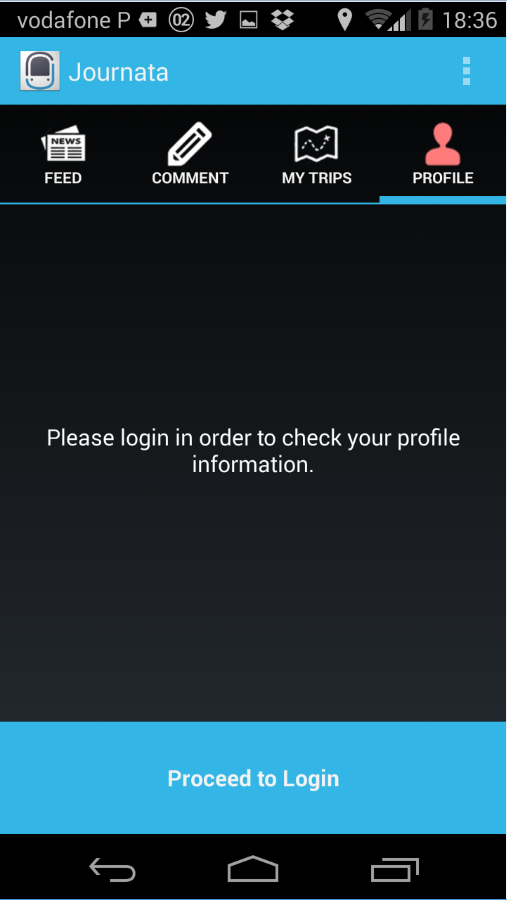
\includegraphics[scale=0.22]{profile_login.png}
    \caption{User profile screen - an example where authentication is required in order to access the information.}
    \label{fig:auth1}
  \end{center}
\end{figure}

In the login screen, a simple form asking for username and password is encountered, as well as the submit button for that form, and a button at the bottom of the screen that redirects the user for the register screen.

\begin{figure}[h!]
  \begin{center}
    \leavevmode
    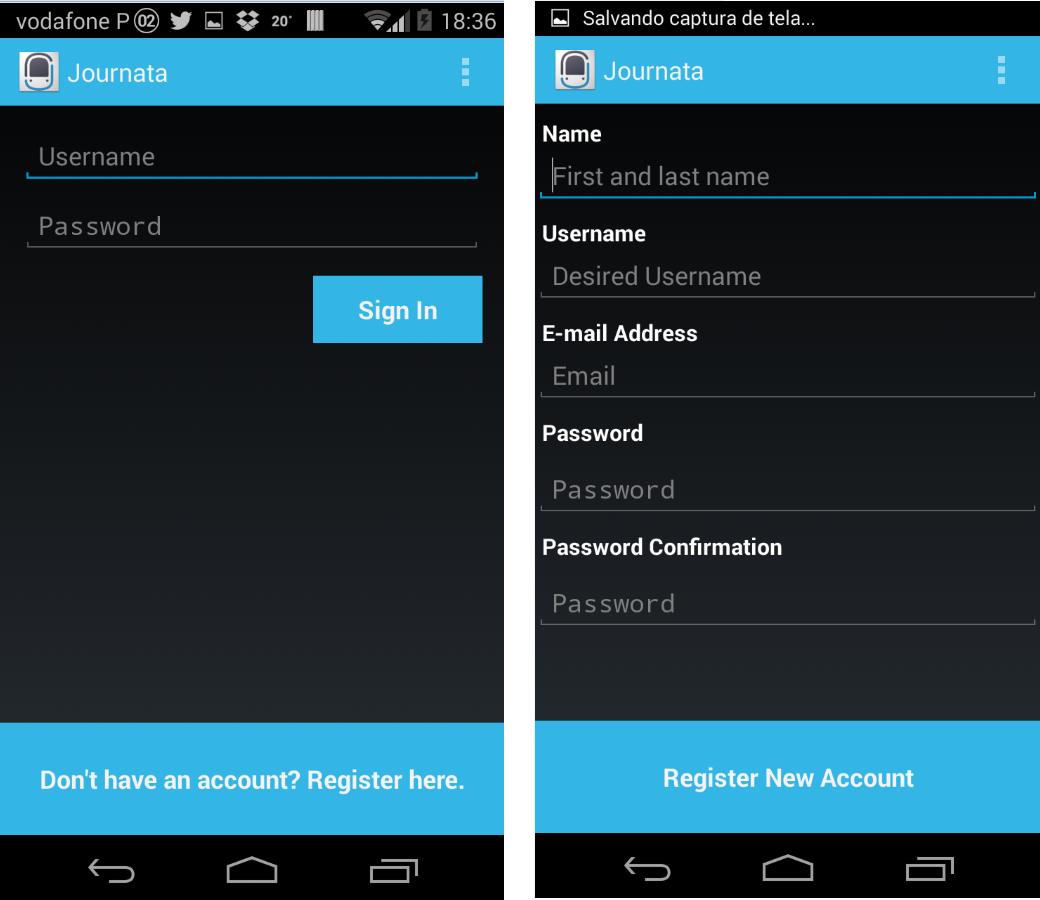
\includegraphics[scale=0.5]{login_register.png}
    \caption{Screenshots of the login and register screens.}
    \label{fig:auth2}
  \end{center}
\end{figure}

Other guidelines were followed in this process. The register form fields were reduced to the very essential - name, username, email, password and password confirmation - in order to reduce the text input effort from the user. The registration form in the previous prototype had two additional fields, nickname and the privacy setting. As for the first one, it may lead to a redundancy with the existing username field (when the privacy setting for the user is set as visible, instead of the nickname, the username field can be shown as there is no need for two distinct fields). 

Regarding the privacy setting, there is no need to define it so soon and introducing that effort on the registration form. Instead, it was assigned a default value for new accounts (public setting, but it can be easily modified in order to make that default the private setting) for the sake of demonstration in this prototype.

The submission of the registration form also triggers a login process after a successful registration. In short, after registering a new account, the user does not need to login and enter their data again, contrasting to what happened in the application developed in the previous iteration of the project.

The use of the \emph{Android} Action Bar as part of the interface allowed to create another options for logging in and logging out of the application, through the creation of an action menu where we can find login and logout buttons.

\begin{figure}[h!]
  \begin{center}
    \leavevmode
    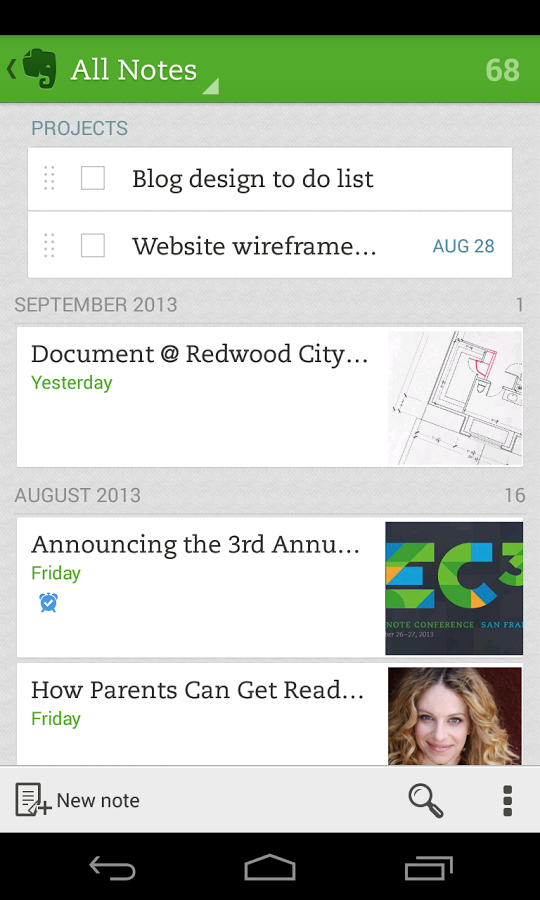
\includegraphics[scale=0.45]{auth1.png}
    \caption{Login and logout buttons in the Action Bar.}
    \label{fig:auth3}
  \end{center}
\end{figure}

Another concern during the development was the persistence of data after pausing or exiting the application. In the implementation of the prototype, all the data regarding the user login and profile is stored locally, in order to be accessible when entering the application again, after pausing or closing it. That said, the application does not require the user to login again after the first utilization (unless, of course, the user logs out in order to use other account).

\newpage

\subsection{Comment Submission}\label{comment}

The submission of comments was always based in the assumption that the user would need to be checked-in in a network, and therefore would need to be logged-in in the application in the first place. 
The features associated to this concept have somewhat not changed too much since the first design performed in this work.

The main interaction flow conceived was the following:

\begin{itemize}
\item Check-in on a network - this would consist in selecting an origin and destination, in a very similar process for what is necessary to add a feed subscription.
\item The main comment menu is presented to the user. In this menu, the user can choose to submit a written comment or to choose one of the previously defined categories of comments, pressing the button for the desired category.
\item A dialog would be presented to the user, containing the several aspects the user can classify inside the chosen category. For each item, a slider with several possible values and a submit button is available, so that the user can submit his feedback for every value individually. The selected value, for the selected aspect, is then converted in a textual comment that will be submitted to the network's news feed. The choice for a dialog, despite not being exactly a good usability guideline, went through because it would allow the users to easily dismiss the dialog and change for another comment category, saving them the effort of navigating for a different screen and then go back if they wished to comment on an aspect from a different category.
\end{itemize}

\subsubsection{First Iteration}

As mentioned before, the first design iteration after the focus group assumed that several simultaneous check-ins from the same user were possible. For that matter, after the first step of performing the check-in, the user would need to choose what was, from within the several simultaneous check-ins, the network where he is in the current moment, in order to submit information to that network.
This was meant to be done in the main comment menu. A spinner would present to the user all the existing check-ins, from where he would need to choose the right one (figure \ref{fig:comment_iter1}).

\begin{figure}[h!]
  \begin{center}
    \leavevmode
    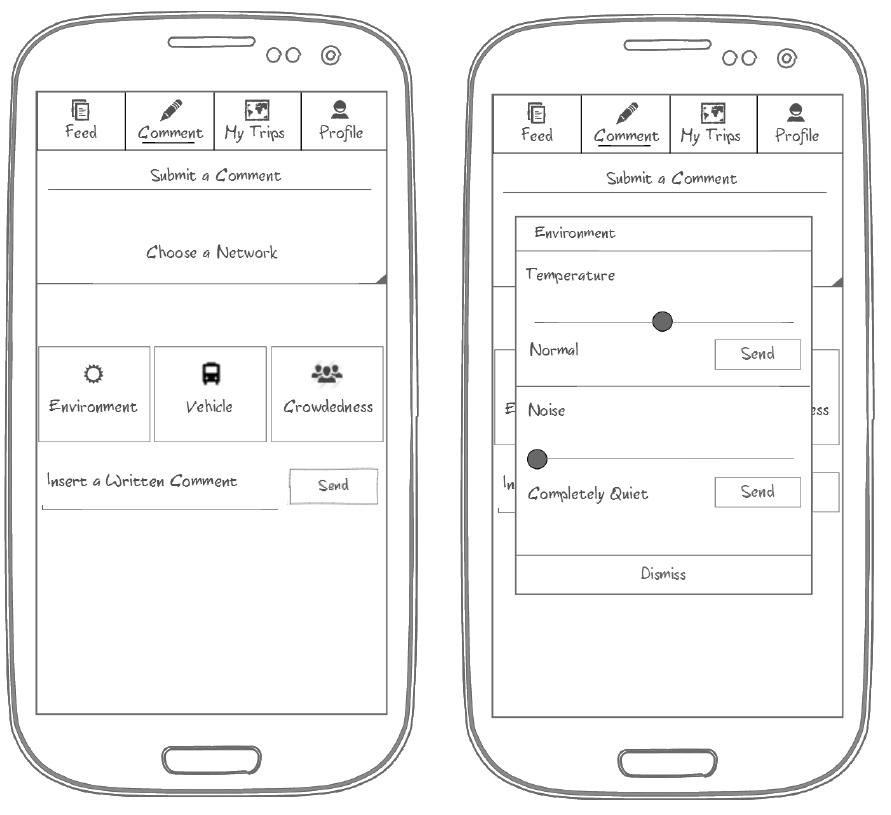
\includegraphics[scale=0.5]{comment_iter1.png}
    \caption{Comment menu - First Iteration.}
    \label{fig:comment_iter1}
  \end{center}
\end{figure}

The chosen method to submit a written comment was to have a text field, along with a submit button, in the main comment menu, so that the task of entering and submitting that type of comment would require as little time as possible.

\newpage

\subsubsection{Second Iteration}

Having simultaneous check-ins posed yet another problem, and this one related with the comment submission. If the user could choose a network from his checked-in networks to mark as the 'current one', and submit information to that network, there would be no guarantee that the user is currently performing that journey, existing the possibility to him to submit information for all the networks he wants. This was another reason that led to the regression (at least in what concerns to comment submission) to a 'single check-in' system.

The spinner mentioned in the first iteration would then be replaced for the information about the network (origin, destination, transportation method and route, when applicable). This would also require the creation of an intermediate screen between the check-in and the comment menu, where the user selects the transportation method and route where he's travelling, because the revised concept of network for this second iteration implies the network includes any option and route between the selected origin and destination, but the information about the vehicle route will be relevant for users seeing the submitted comments in their feeds.

\begin{figure}[h!]
  \begin{center}
    \leavevmode
    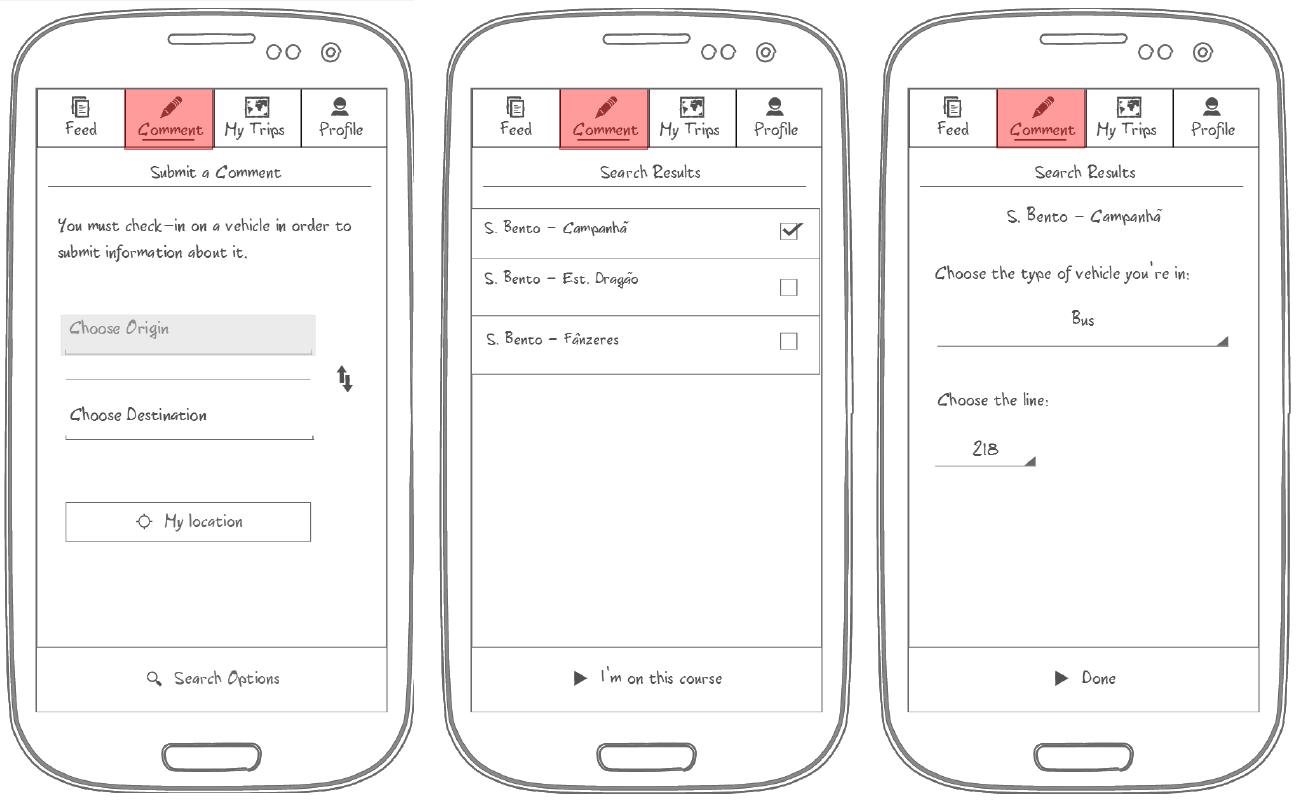
\includegraphics[scale=0.48]{comment_iter2_1.png}
    \caption{Check-in and definition of route - Second Iteration.}
    \label{fig:comment_iter2_1}
  \end{center}
\end{figure}

\begin{figure}[h!]
  \begin{center}
    \leavevmode
    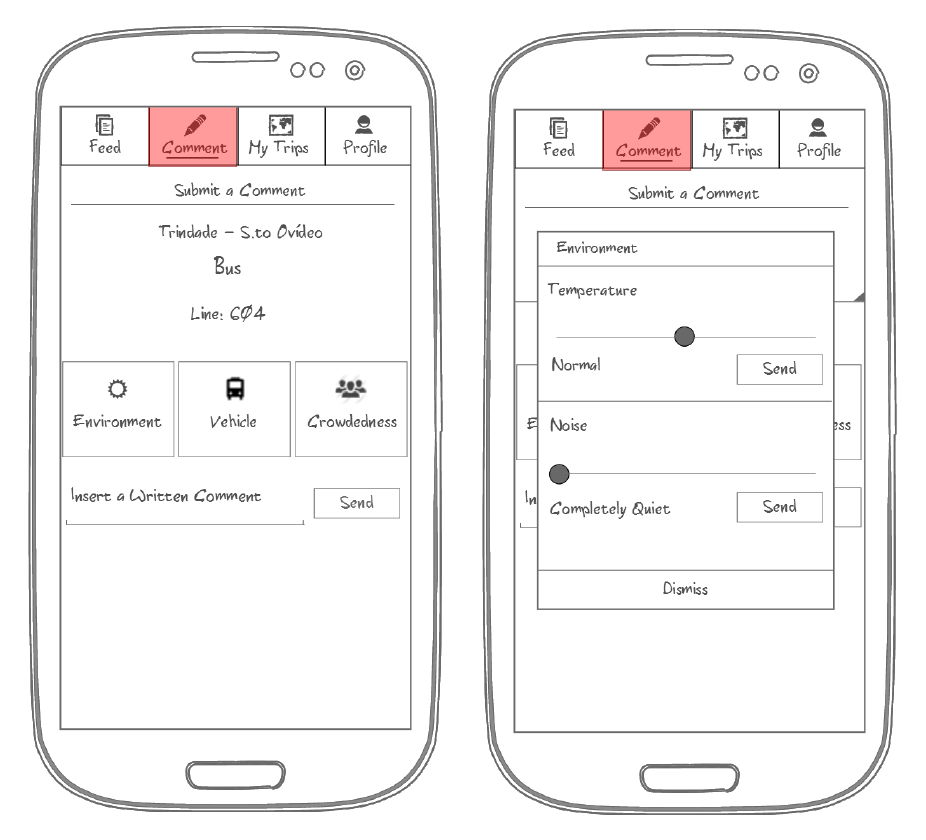
\includegraphics[scale=0.48]{comment_iter2_2.png}
    \caption{Comment menu and classification dialog - Second Iteration.}
    \label{fig:comment_iter2_2}
  \end{center}
\end{figure}

\newpage
\subsubsection{Implementation}

The implementation of these features tried to follow as much as possible what was established in the second design iteration. The only difference to register is that the intermediate step, where the user defines the route where he's travelling, was not necessary because the current representation of a network included only a route and direction, and the only transportation method in the database is bus, there was only a choice to be made in that screen if it were implemented. For this prototype, it was decided not to.

\begin{figure}[h!]
  \begin{center}
    \leavevmode
    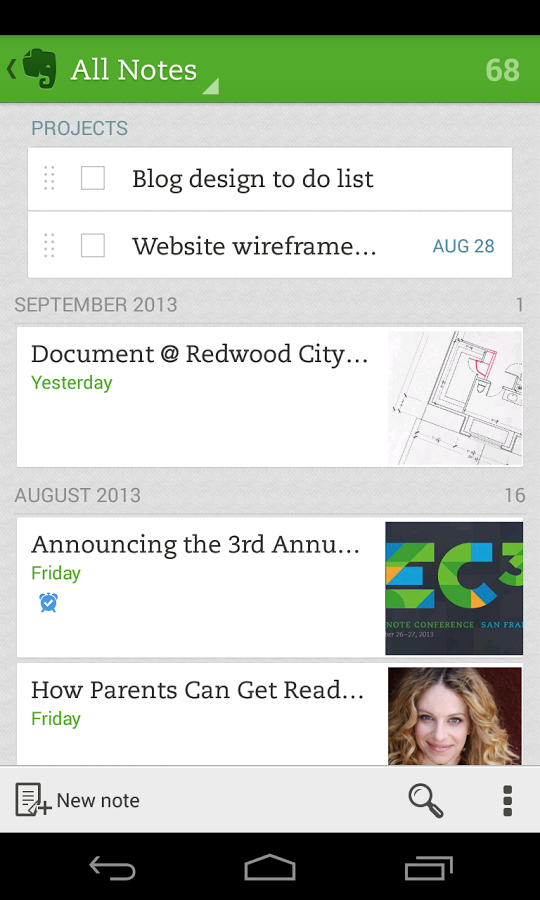
\includegraphics[scale=0.45]{auth1.png}
    \caption{Screenshots of the implementation of check-in and comment submission features.}
    \label{fig:comment_impl}
  \end{center}
\end{figure}

The check-out feature was also implemented, and can be encountered in the menu available in the Action Bar. Performing the logout action while checked-in will also trigger the check-out action.

\subsection{Journey Planner Features}\label{journeyplanner}

For this module, the suggestions given by users on the focus group session were crucial to the definition of the following features:

\begin{itemize}
\item \textbf{Favourites} - User adds a feed subscription (through a similar workflow used to add a feed to the current subscriptions) to a list of his favourite feeds. In that list, user can easily activate any of those feeds through pressing a checkbox. This way, a user does not need to be constantly adding and removing the same feed subscription everytime he wants to receive information for a given journey that he happens to do with reasonable frequency.
When a favourite feed is activated, is it automatically added to the current subscribed feeds (along with the others added on the 'Feed' module of the application).
\item \textbf{Schedule} - Allows the user to see a list of journeys he planned for the future, with the associated date and time. The journey planner features that made part of the previous developed prototype \cite{kn:Gon12} were included here in order to be possible to add new plans to this schedule.
\end{itemize} 

The journey planner, as it was initially conceived, was also intended to send notifications to the user ten minutes before a planned journey was scheduled to start, in order to ask to the user if he wanted to receive information from the corresponding network. 

With the deprecation of \emph{Google Cloud to Device Messaging Framework}, these notifications were eliminated, and the idea was to automatically add the feed subscription for the network referring the planned journey to the list of current feed subscriptions, activating that feed as a default. That action would be triggered 30 minutes before the planned start time for the journey, so that the user can receive some information beforehand about what is happening in the network, and it would be automatically deactivated one hour and a half later (it could also be manually deactivated as well).

\subsubsection{Iterations}

The difference between the two main design iterations happened in the screen where the used could plan a new journey (in other words, add a new journey to the schedule).

\begin{figure}[h!]
  \begin{center}
    \leavevmode
    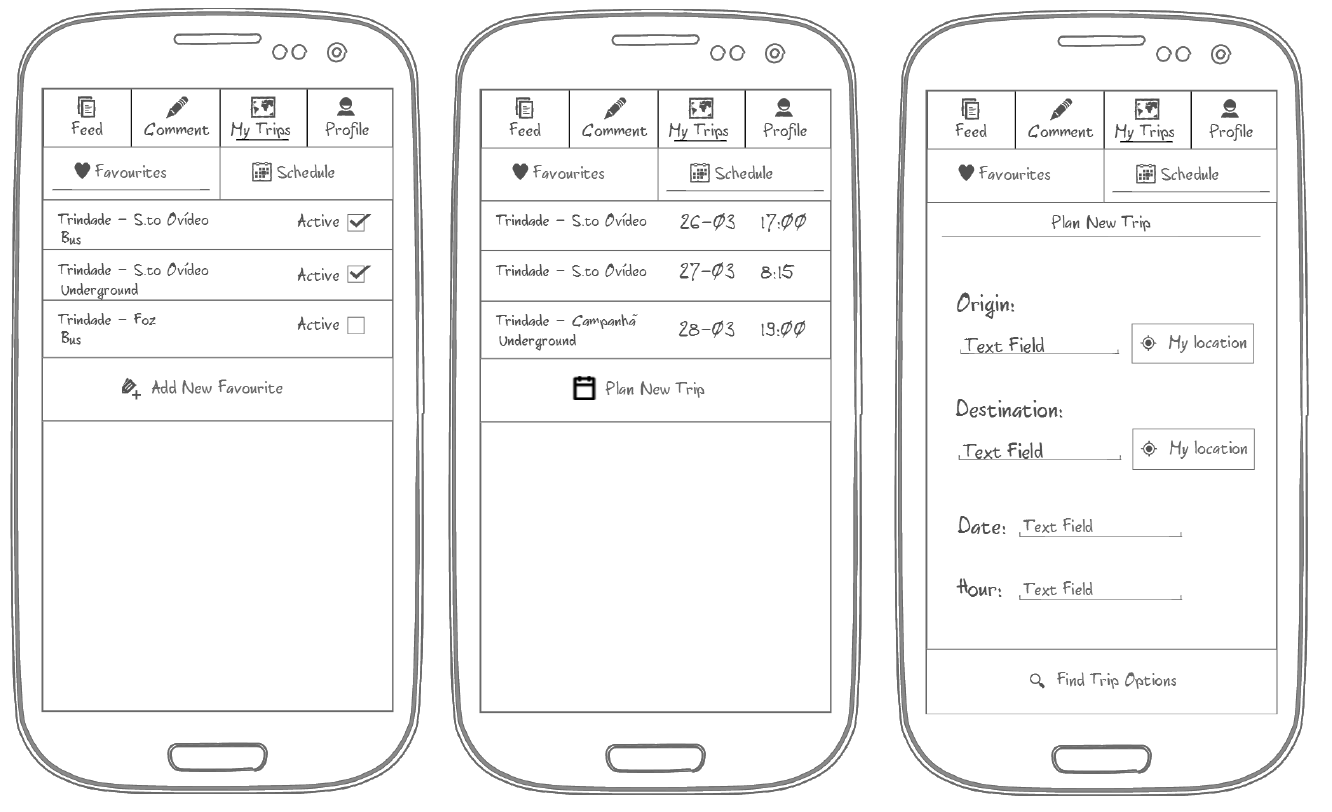
\includegraphics[scale=0.5]{planner_iter1.png}
    \caption{Favourites and Schedule features - First Iteration.}
    \label{fig:planner_iter1}
  \end{center}
\end{figure}

For the second iteration, it was decided not to limit the selection of the date of a planned journey to a single day, and to allow planning of repetitive tasks (very similar to what is allowed in alarm applications), selecting the days of the week when the user plans to do the journey.

About the introduction of text in the origin and destination fields, the same principles applied in similar tasks in the application were also applied here, with the existence of auto-complete and the button to switch the origin and destination fields content.

\begin{figure}[h!]
  \begin{center}
    \leavevmode
    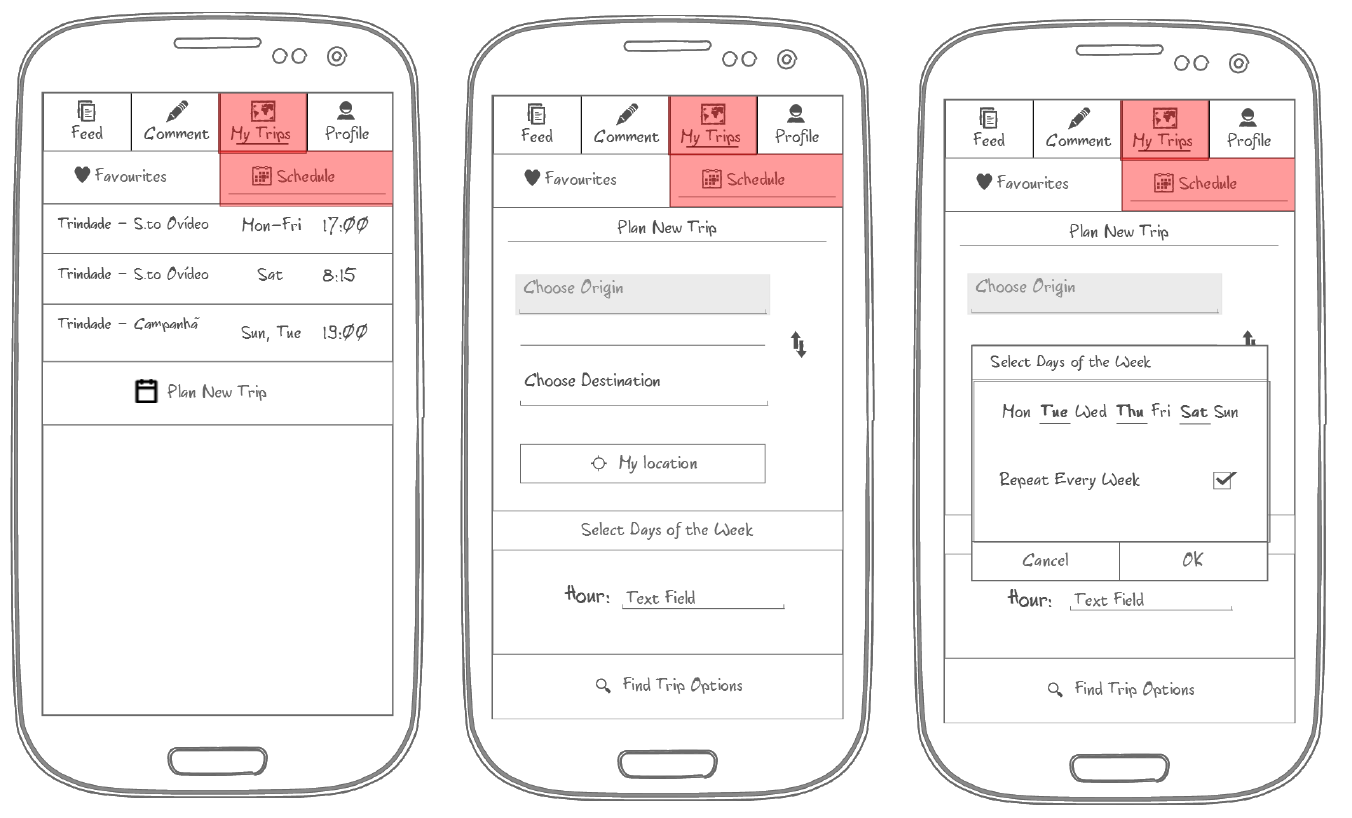
\includegraphics[scale=0.5]{planner_iter2.png}
    \caption{Favourites and Schedule features - Second Iteration.}
    \label{fig:planner_iter2}
  \end{center}
\end{figure}

\subsubsection{Implementation}

The implementation followed what was established in the design phase. However, there were room for some changes, such as fixing the position of the buttons at the end of the lists (favourites and schedule) in order to be coherent with the implementation of the remaining modules and allow the user to perform the majority of the main application flow through the press of well-sized buttons at the bottom of the screen.

An external library was also used to help with the implementation of the date (with repetitive tasks) and time 'pickers' for the journey planner, \emph{DateTimePicker}\footnote{\url{https://github.com/flavienlaurent/datetimepicker}}, that contained the attractive widget for those type of tasks that is also possible to find in the most recent versions of \emph{Google Calendar} application.

\newpage

\begin{figure}[h!]
  \begin{center}
    \leavevmode
    \includegraphics[scale=0.5]{auth1.png}
    \caption{Screenshot of the implementation of the favourites and schedule lists.}
    \label{fig:planner_impl}
  \end{center}
\end{figure}

\newpage

\subsection{User Profile}\label{userprofileimpl}

After the focus group and the fears shown by the users regarding seeing other users in the same network and having his own data (despite limited) possibly visible to other users, it was decided to change the information displayed in the user profile screen to match some of the suggestions given in that session, such as user statistics, along with some of the initially predicted information to be displayed:

\begin{itemize}
\item Username
\item Points
\item Stars
\end{itemize}

The additional information selected, apart from user statistics, was:

\begin{itemize}
\item List of available rewards (claimed with points).
\item User photo (with the option to upload a new one).
\item Option to change privacy settings (changing the visibility of username and photo).
\end{itemize}

In a first draft, it was also considered the inclusion of a check-out button in this screen, but that option was discarded because it was believed that it made little sense to have that option in this tab due to low visibility to the user.

After that decision, there would be no changes at all to the interface designed as a first iteration.

\begin{figure}[h!]
  \begin{center}
    \leavevmode
    \includegraphics[scale=0.45]{profile_iter1.png}
    \caption{User Profile screen - Design phase.}
    \label{fig:profile_iter1}
  \end{center}
\end{figure}

\subsubsection{Implementation}

The implementation phase for the user profile module followed the interface conceived in the design phase. However, due to the reformulation in the points system (see section \ref{points}), the information about the stars given to the user was replaced by the information about his feedback points.

\begin{figure}[h!]
  \begin{center}
    \leavevmode
    \includegraphics[scale=0.45]{auth1.png}
    \caption{Screenshots of the implementation of user profile screen.}
    \label{fig:profile_impl}
  \end{center}
\end{figure}

The privacy settings feature was also moved to the \emph{Android} Action Bar, giving his place in the screen to a button that allows the user to see his statistics.

 
\chapter{Tests and Results} \label{chap:chap6}

\section*{}

The tests presented in this section aimed to evaluate the quality of the interface and interaction developed as the result of the process detailed in Chapter \ref{chap:chap5}. 

It also aimed to gather some conclusions on perspectives to the evolution of the application, such as future integration with larger-scale applications or projects in the public transport applications field.

\section{Usability Test}

The work performed during the design phase, as established in Chapter \ref{chap:chap5}, led to deep changes regarding the application features, navigation and the concepts behind the application. To validate those concepts before the implementation phase, it was decided to perform an usability test.


During one week, some people were asked to use a low-level prototype and try to accomplish a predefined set of tasks, and give their feedback about the application and their possible difficulties in grasping the concepts behind it, in a controlled environment.

To guide users during this test, a script was presented to them (see Appendix \ref{ap2:usabtest}). This script was divided in two parts, a first one presenting a set of specific tasks to be accomplished through navigation and a second one where some questions to collect feedback about certain aspects were asked to the testers.

Following Jakob Nielsen's recommendation for qualitative user research \cite{kn:MobileUsab}, this test was presented to 6 subjects, with the majority of them being different from those who were in the focus group session previously made.

All of them are frequent public transport users and reside in the Porto Metropolitan Area, have a smartphone and have ages comprehended within 18 and 25 years old. It was attempted to have a equal gender distributed sample , but that was not achieved in a timely manner. The sample ended up having 67 percent male subjects and 33 percent female subjects.

The presented set of tasks included: 

\begin{itemize}
\item Adding new feed subscriptions.
\item Filter the visible feed subscriptions.
\item View feed information.
\item Remove a feed subscription.
\item Rate another user comment.
\item Submit a written and a categorised comment.
\item Check the favourite journeys.
\item Check the scheduled journeys and add one journey to that list.
\item Check the user profile.
\item Check the rewards list.
\end{itemize}

The users were also asked to classify the perceived difficulty (from 1 to 5, where 1 represents very difficult and 5 represents very easy) of the interaction for each task and to assess the clarity of the messages and text presented by the application.

The set of tasks that included adding a new feed subscription were perceived as easy. However, despite that perception, there were some difficulties in understanding the meaning of the concept and what information was included in the feed. After understanding, however, the subjects appreciated the simplicity of the task. This task had an average classification of 4.3 out of 5.

Both the filtering and removal of feeds were perceived as very easy to do and to understand. However, it was observed that the users took some time to figure out how to perform the removal of a feed, because there is no indication or visual element indicating that this is an option. All the subjects, however, assumed after that additional time that there would be a menu available after a touch on an item of the list, but that is possible related to the existing experience with smartphones from those subjects. The average classification for the filtering task was 5 out of 5, while the removal task had an average classification of 4.5 out of 5.

Viewing the feed information as perceived by the users as a simple and attractive task, especially due to the text representation of categorised comments in the feed and to the information elements that identified the specific journey from where the comments are submitted. The average classification for this task was 4.9 out of 5.

The rate comment feature, despite the fact that the users considered the interaction that leads to it as easy to learn, there were difficulties in understanding what that feature would do, and why would the users 'need' to rate other users' comments, specially as they didn't receive any reward from that. The average classification for this task was 4.7 out of 5.

Submitting a comment was perceived as a task of very reduced difficulty, and good feedback about the transition between producing a categorised comment and switching back in order to choose another category or to submit a written comment was received. The average classification for this task was 5 out of 5.

Both the favourites journeys and schedule features were perceived as very useful and with simple interaction, since they are as well available in other applications. The option for setting a scheduled journey as a possible repetitive task, for certain days of a week, for example, was seen as very useful and very easy and intuitive. 
The average classification for this task was 4.7 out of 5.

Checking the user profile was one of the tasks perceived as more obvious, as well as checking the list of possible rewards. Both the 
tasks had an average classification of 5 out of 5.

Therefore, it was concluded that it was necessary to redesign the rate and points system in order to make it attractive to the user to understand. An easier definition of that system, perhaps related to another feedback system widely used in other social websites or applications, would provide that better understanding and probably captivate the user to give feedback about other users' comments. It would also be useful to arrange a way to allow easier understanding of the concept of feed subscription and the amount of information associated to it. This aspects would had to be taken under consideration in the implementation phase.

\section{Evaluation by Experts}

In the end of the implementation phase, a session for evaluate the usability and interaction of the obtained functional prototype was held at OPT's offices, in Porto. 

Five of the company's experts on usability and application development for public transports (both mobile and web applications) were present in this session, to act as experts and provide feedback about the developed application.


To the experts, it was provided the script used in the usability test previously performed with users, and a brief session was held before the evaluation to explain some of the concepts behind the applications and some of the changes occurred during this process.
After that brief introduction, all of the experts were asked to freely explore the functional prototype of the application, while observed by the author of this work, in order to register the problems encountered, the suggestions and to discuss possible improvements.

Some test accounts were created before the session and their authentication credentials were provided to the experts, despite the fact that they were also encouraged to create new accounts if they wanted to.

There were also provided some routes with a vast amount of existing information in the application database as a suggestion in order to give them full utilization experience of the application.

\subsection{General Evaluation}

The general consensus among the experts was that this was an application very easy to use, with a 'linear' navigation in most cases, with the flow between screens inside an use case occurring through a button on the bottom of the screen.

Despite that, several usability and interaction problems were detected during the session (some of them related with bugs in the implementation):

\begin{itemize}
\item When the user initially enters the application, an information that he has no feeds subscribed is displayed. However, and in contrary to what happens in other modules of the application, there is no button in the bottom of the screen redirecting the user to that feature, causing some confusion on the user regarding the existence of a trigger on clicking the displayed information text or leading him to explore other features inside the module and wasting unnecessary time in navigation.

\item Regarding the comment submission module, some messages displayed to the user had the wrong information, and others did not make the process of user checking-in on a network before comment submission explicit enough. Despite not having great influence in the user perception of the feature, it does not give him the perception that he is checked-in and he can perform check-out. This is amplified by the fact that the access to the checkout feature is hidden on the Action Bar.
One suggestion to solve this problem is to take advantage of the existing free space on the main comment menu and add a button allowing the user to perform check-out.

\item The position of the text field to submit a written comment is causing the \emph{Android} keyboard to hide its content, forcing the user to write his comment 'blindly'.

\item The selection of items in lists of results (adding a feed, for example) has a problem regarding consistency of interaction. The existence of a checkbox leads some users to click inside the checkbox or to click the list item. Due to problems during the implementation, a decision was made in order to associate the selection to the click of the bigger target (the list item), since the checkbox has a reduced size. However, the users who clicked inside the checkbox had problems, and improving the consistency between the two types of interactions to change the selection state is required.

\item The auto-complete feature should return the options that do not necessarily start with the introduced text, but those who contain it.

\item The upvote ('thumbs up') and downvote ('thumbs down') buttons size was perceived as too small and too close from each other. Displaying the feedback points from a comment would be a good information to show along with the buttons.

\item The text representation of categorised comments can be improved for readability. The representation used as an example in the prototypes from the design phase were perceived as better when comparing to the representation used in the functional prototype.

\item A timeout should be implemented for the written comment submission and for each item in the categorised comment submission, to avoid possible \emph{spamming} of comments in the platform.

\item A 'send all' button should be introduced at the end of the categorised comment categories dialogs in order to save some clicks to the user (a timeout should also be implemented).

\item More thought should be put on the location of the favourites and scheduled list. Since they are now the centerpiece and moved the journey planner to the background (as a method to use those features, and not as the feature itself), and since they are related with feed subscription (it is essentially a list of favourite feeds and a feed subscription scheduler), perhaps they would be better located if they were in the 'feed' module, but that would also imply having too many features concentrated in that navigation tab.
\end{itemize}

Concerning difficulties from the users in grasping the concepts behind the application, it was recognized by the experts that one of the more important and difficult questions raised by the application resides in the way to identify the specific vehicle where the users who comment are travelling, in order that the user receiving information can understand what vehicle is mentioned in the comments (this gains even more importance in high frequency routes or services).
About the feed subscription concept, a recommendation was given in order to simplify it and limit the feed to courses with monomodal transportation and without changing routes/lines. That would represent the majority of the journeys and facilitate the understanding of the concept for a big number of users. The remaining ones would need to add several feeds instead of one, depending on their course. This would also make the user have less course alternatives and receive less (and possibly more relevant) information when performing long multi-modal journeys.

The new rating system was appreciated by its simplicity (and the several limitations of the previous system were also recognized and discussed). Some possible future improvements of the new system were also suggested, such as the implementation of point rewards for 'thumbs-up' or 'thumbs-down', since the users are performing the comment validation for the platform, and also that the understanding of those actions should be clarified, in order to represent more like an agreement with the submitted comment and less like a 'like/dislike'. This way, a user would be lead towards not submitting a comment with the same information that was already submitted (because that would award him points) and less redundant and more reliable information would be produced.

\subsection{Suggestions and Observations}

The following suggestions were also given by the experts (some of them were the subject of discussion about how they could work and some of the trade-off involved):

\begin{itemize}
\item Aggregating more than one 'reviewed' aspect in just one comment (making the current comments information 'chunks' of a bigger comment) would be a nice thing to introduce. It would reduce the quantity of request from the application to submit a comment, and it could be presented as only one item in the feed. 

Currently, if the user wishes to submit a comment about several aspects, submitting them individually, other user who wants to check the network feed information would have to scroll to see information submitted by other users because he would see several items in the feed referring to those several submissions, when he could be seeing just one item (that he could click to see in detail).

\item Swipe gesture should not only navigate between tabs from the primary navigation, but also the secondary one. For instance, if the user is in the 'View Feed' screen, a swipe to the left should lead him to the 'Select Feeds' screen, and not to the 'Comment' tab. Only if the user is on the 'Receive New Feed' (the last one on the secondary navigation for the first tab) and performs the same gesture should he be led to the 'Comment' tab.
\end{itemize}

To conclude this section, two additional observations during the tests were registered by the author:

\begin{itemize}
\item Despite having the possibility to navigate between tabs by using swipe gestures, users almost always used the click on the desired tab to navigate.
\item All the experts expected an action by clicking on a comment item on the view feed feature. It was unsure if this was caused by the background color on the comment text, but this remark can be used along with the 'aggregated comment' recommendation given above to serve as a possible positive feedback of the implementation of that feature. It shows that the visible metaphor seems to be there already for the users, but with no functionality.
\end{itemize}
\chapter{Conclusions and Future Work} \label{chap:chap7}

\section{Conclusions}

Usability does not give exactly magic formulas, rules and processes that should be followed every time to get a good and intuitive application, product or solution.
It includes a wide set of recommendations, guidelines and other methods, based on extensive research, that can lead us to a better final result, but there also lots of trade-offs to be discussed in the process of developing such application or product.

In the context of an ongoing project \cite{kn:NGeCP11}, the main goal of this work was to provide better interaction and usability to a innovative mobile application, dedicated to sharing information on public transports \cite{kn:eSG12}, through the definition and application of a user-centred design process. The mentioned application introduces a change in the public transport information system, providing travellers data that is fed to the system by other travellers. To avoid irrelevant and unnecessary information to be shown to a traveller, this application relies on the creation of temporary networks composed by the most relevant passengers at a given time, improving the time and space relevance of said information.

In a first phase, this work aimed to elicit usability requirements for the application among potential users. This stage was performed by holding a focus group session to discuss what the users wanted and ways to improve their engagement with the application and make their understanding of the concepts behind the application much easier.

That initial phase, however, revealed that, in order to achieve those goals for the application, some profound changes about the said concepts were necessary, which resulted in an extended design phase comparing to what was predicted. 
The result of the design phase, however, was richer and considered a great step to the potential success of the application, as validated through usability tests (see Chapter \ref{chap:chap6}).

Those tests gave then place to an implementation phase that resulted in a functional prototype, \emph{Journata}. This functional prototype was then tested with experts (also mentioned in Chapter \ref{chap:chap6}), since a test with real users would be a time consuming task which was postponed to a forthcoming phase. 

The results of that session were very satisfactory and assessed that this work is a big step in the right direction, but also there is yet a lot to be done and explored (as it can be seen in the following sections). This was seen as a big motivation to keep working in this concept and a confirmation of the huge potential of this application and the influence it can have on solving mobility problems and improving public transportation usage experience.

\section{Future Work}

Despite the fact that this work can be considered a big step to the fulfilment of all the recognised potential in the application (and possibly helped to figure out solutions to make that potential even higher), there is still a long way to go regarding that matter, and several features regarding usability and architecture of the project can be object of future work.


It must also be said that the potential from this application and project was also recognised by external entities, that want \emph{Journata} or some of its features to be included in a bigger scale project regarding a mobile payment solution for public transports, that intends to dematerialize the public transport tickets. 
The author of this work was selected to be part of that project, where he will have the opportunity to work on the integration of the information sharing features on such a innovative platform for the public transports 'big picture' in Portugal.
He will also have the opportunity to continue the work performed on this thesis and achieve some of the points mentioned in the following sections, while trying to follow the suggestions obtained in the test phase.

\subsection{Usability and Interaction}

Apart from following the suggestions given by the experts on the evaluation session (see Chapter \ref{chap:chap6}) and implementing the features referred in the designed phase that, due to time constraints, were left aside, the following work could also be done:

\begin{itemize}
\item Develop an interface layout for landscape view for the entire application.

\item Create alternative locations (translations) and themes for the application. 

\end{itemize}

\subsection{Data Structure}

%However, a problem that was not possible to overcome in a timely manner was that the existing data structure for representing the networks did not allow to fetch the origin and destination of those networks in the feed, despite what has been discussed in the design phase. The only useful information that can help the user identifying the network the information refers to is the number of the bus route (the current data set used only bus stops and routes from the city of Porto). This is expected to be corrected in a near future.

In order to fully implement the concepts of the application as they were conceived during the design phase of this work, profound changes to the data structure behind the application are necessary. 

\begin{itemize}
\item Implement the new point system and support the reward model.
\item Networks should not be entities associated to an unique route or direction. They should be, instead, associated to one user, and to the origin and destination of the journey performed (or intended to be performed) by that same user, containing users in relevant routes to the user journey. 
Some of the limitations of the current structure formed an obstacle when implementing the 'view feed' feature, leading to the impossibility of displaying the information thought to be displayed to the user in the design phase. However, those limitations go much further than that and a rethought implementation of networks in the system should be subject of an in-depth discussion.

\item Requests for feed information should be specified through the utilization of a range of time for the desired information, instead of getting only the information since the last request.
\item Support a way to the transport providers to send relevant information about some routes through the application.
\item Provide techniques that allow the deduction of travel patterns from the users, which could be used to automatically add or suggest new feed subscriptions to the user based on the gathered information.
\item Improve the security of the application denying non-authorized access to data that does not require a login state. 
\end{itemize}

\subsection{Integration with existing social networks}

Despite the fact that some of the social features considered in the initial phase of this work were left aside, due to concerns shown by the users, there is still possible room to be explored here concerning the integration with existing social networks. 

One possible way is to provide means to register in \emph{Journata} through the use of an account from a widely used social network, such as \emph{Facebook} or \emph{Twitter}, saving the effort to create an account manually.
Other possibility is the use of the said social networks' friends list to provide the initially thought social features for \emph{Journata} (nearby users, checking other user profile and so on) only for those users who are part of those lists, and also use \emph{Journata}.
Some work on user statistics and exploring ways to integrate them with gamification concepts could also be used to allow the user to share his data into his social networks' accounts.


\subsection{Integration with existing public transport applications}

It would present an advantage to the application if it could be integrated with a system that acted as a substitute for travel tickets. For a start, a validation at an entering and exiting stage from a journey or vehicle (taking advantages of technologies such as NFC or QRCode) would dismiss the necessity of a check-in or check-out features, as it would be an automatic validation process, and it would also allow the gathering of data for deduction of travel patterns.

\emph{Journata} would also have a lot to gain with the integration with services such as the API used by MOVE-ME \footnote{\url{http://www.move-me.mobi/}} as a source for its auto-complete and journey planner features, as it contains not only the bus, train and subway stations, but also information and location of interest points that could also be set as origins or destinations for journeys. This specific API is obviously only for a limited scope of \emph{Journata}, concerning the data of the city of Porto. 







%%----------------------------------------
%% Final materials
%%---------------------------------------

%% Bibliography
%% Comment the next command if BibTeX file not used
%% bibliography is in ``myrefs.bib''
\PrintBib{myrefs}

%% comment next 2 commands if numbered appendices are not used
\appendix
\chapter{Focus Group Script} \label{ap1:focgr}

\subsection{Goals}

This \emph{Focus Group} intends to present some uses cases from the application, in order to elicit usability requirements for a future functional prototype of the said application.
It is intended to promote a discussion which, recurring to suggestions of interface designs for some of the use cases, can serve as indication to the best way to proceed regarding the interaction of the application.

\subsection{Briefing to the participants}

A number increasingly higher of public transport passengers is connected everyday to social network platforms through the utilization of their personal mobile devices. This allows sharing of information between passengers in real time, regarding several aspects of the public transport service at a given moment.
This kind of information can be useful both to the users, in order to help them take more informed decisions regarding their journeys, and the transport network managers, helping them to introduce improvements to the service.
Regarding this last point, there can also be benefits to the public transport operators through the acquisition of operational information in a more timely manner and with less use of resources.

However, the most used social networks are incapable of aggregating and distributing custom information to passengers and managers of public transport networks, leading to the existence of spread information with much less utility. Therefore, it is intended to develop a prototype of a mobile service based on the structure of a social network, but innovative in the way how users are connected between each other, temporarily, based on their location and travel patterns. 

The developed prototype will be a new and more advanced version of other prototype previously developed, but with significant improvements in several aspects, such as usability and the capacity to establish temporary connections between passengers in an intelligent and real time manner.

\section{Use Cases to Discuss}

\subsection{Journey Planner and Check-In}

\begin{itemize}
\item Check-in must have better visibility than in the previous prototype. In that prototype, the journey planner, despite referring to a probable check-in in a future journey, had more visibility than a journey intended to perform in the immediate present.

\item It is impossible to verify is the user has several trips planned (it is not possible to list all the previously planned journeys), which brings up a difficulty if the user had planned more than one trip to perform in the future. The implementation of such feature has benefit?
\end{itemize}

\subsection{User Profile}

Displays information about the user profile in the application. Suggestions for data to display in this screen are:

\begin{itemize}

\item User Name
\item Photo/Avatar of the user.
\item Map with user location (and possibly users in the same network).
\item Information about vehicle or route where the user currently is.
\item Menu to access other features.
\item Access button to visibility/privacy options.

\end{itemize}

Regarding this use case, other questions that may be relevant of discussion:

\begin{itemize}
\item Is the user profile screen the best to display to the user when entering the application (instead of, for instance, travel information)?
\item Access to other features should be made from this screen or should the other feature be accessible on other 'tabs' from the application or through a swipe gesture?
\item Is this the right screen to display points and stars from the user?
\end{itemize}

\subsection{Trip information}

Regarding this use case, the following points must be considered:

\begin{itemize}
\item \textbf{Information displaying mode} - Should be implemented, for instance, under the form of a 'newsfeed' or there is a better way to do it? The task of 'rating' the information should be in another 'tab', to give visibility to that feature, or done recurring to buttons appearing in the news feed along with the information?

\item \textbf{Easiness of information submission} - The user must have minimum effort to submit new information. This means that the interface for quantitative rating of information should be as  clear as possible (with properly sized buttons or through sliders). The qualitative information submission (written comments) should also minimize text input effort from the user.

\item \textbf{Presentation of the types of information to submit} - Previous division by category (such as the previous prototype)? All types of information in the same page/screen (scrolling requires less effort than going back and choosing other category, despite the fact that the items in the end of the list become less visible)?
\end{itemize}

\section{Other questions to discuss regarding other features or interactions}

\begin{itemize}
\item \textbf{\emph{Early Registration}} - Eliminating early registration in the application, giving the user features that do not allow login or check-in in a network to access information could lead to less 'abandon rate' when first using the application.
However, it could lead to a vast number of users not creating an account to share information.

\item How relevant to the users is the possibility to see other users in their temporary network?

\item It would be interesting to provide users with the history of their trips and submitted comments?

\item \textbf{Notifications} - Sending a notification to the user when he enters a network or has a planned journey in the next 10 minutes is excessive?

\end{itemize}



\chapter{Usability Test Script} \label{ap2:usabtest}

\section{Introduction}

This document intends to serve as a script to the realization of an usability test of an interface for a mobile application to be implemented for the \emph{Android} mobile operating system.
This application has features of a social network, and aims at sharing information about public transport networks, with that sharing component being performed by the users of the platform.

This test aims to perform the validation of low-level prototypes developed in order to provide an interface and an interaction flow to the mentioned application.

To the realization of this test, a sequential set of tasks should be performed by the users. It is intended to evaluate the easiness of interaction between the user and the proposed interface, with the purpose of detecting and solving possible problems before an implementation phase.

\section{Socio-demographic questions}

\subsection{Age}
\begin{itemize}
\item 18-25
\item 25-30
\item 30-40
\item 40-50
\item 50+
\end{itemize}

\subsection{Gender}
\begin{itemize}
\item Male
\item Female
\end{itemize}

\subsection{How frequently do you use public transports?}
\begin{itemize}
\item Frequently (1-5 times per week).
\item Often (1-5 times per month).
\item Rarely (1-10 times per year).
\item Never.
\end{itemize}

\subsection{Are you a smartphone owner and user?}
\begin{itemize}
\item Yes.
\item No.
\end{itemize}

\subsection{Please state your city of residence.}

\section{List of Tasks to Accomplish}
\begin{itemize}

\item \textbf{Task 1 -} Add a new feed, entering manually the origin and destination you desire. For the sake of this test, enter 'S. Bento' as the desired origin.

\item \textbf{Task 2 -} Add to of the displayed results to your current feeds (for instance, \textbf{S.Bento - Campanhã and S.Bento - General Torres}).

\item \textbf{Task 3 -} Check the list of current subscribed feeds. Verify that those you added make part of that list.

\item \textbf{Task 4 -} Hide the information from the feed referring to '\textbf{S.Bento - General Torres}'.

\item \textbf{Task 5 -} Remove one of the feeds (\textbf{Hospital S. João - Trindade}). Verify that it's no longer part of the list.

\item \textbf{Task 6 -} Read the information coming from the feeds subscribed.

\item \textbf{Task 7 -} Rate another users' comment.

\item \textbf{Task 8 -} Assume that you've just entered a bus from the route 604, with destination \textbf{Sto. Ovídio}. Submit a written comment about that trip.

\item \textbf{Task 9 -} Submit another comment about the trip, this time regarding the noise on the vehicle.

\item \textbf{Task 10 -} Access your favourite journeys list. Assume that there are already two there (\textbf{Trindade - Sto. Ovídio} e \textbf{Trindade - Foz}). Deactivate the one that is currently active.

\item \textbf{Task 11 -} Check your scheduled journeys. Add another journey to the same list.

\item \textbf{Task 12 -} Consult your user profile. Enter the list of reward to check the discounts you can claim with your current amount of points.
\end{itemize}


\section{Post-task questionnaire}

In a scale from 1 to 5, with 1 representing 'very hard' and 5 considered 'very easy', classify your perception of the difficulty of the task, based on the simplicity of the interaction and the clarity of messages displayed in the interface.

Finally (and optionally) give an answer to these questions:

\begin{itemize}
\item Would you use an application such as this in your daily routine?
\item What captivates you more about the application (one specific feature, the possible rewards, etc.=?
\end{itemize}

%% Index
%% Uncomment next command if index is required
%% don't forget to run ``makeindex mieic-en'' command
%\PrintIndex

\end{document}
